\documentclass[11pt]{amsart}
\pdfinfoomitdate=1
\pdftrailerid{}
\pdfsuppressptexinfo=15
\usepackage[T1]{fontenc}
\usepackage{lmodern,amsmath,amssymb,amsthm,mathtools}
\usepackage[margin=1.08in]{geometry}
\usepackage[expansion=false]{microtype}
\newcommand{\DoNotLoadEpstopdf}{}
\usepackage{enumitem,booktabs,longtable,array,needspace,tikz-cd}
\usetikzlibrary{arrows.meta,positioning}
\usepackage[hidelinks,pdfusetitle]{hyperref}
\usepackage[capitalise,noabbrev,nameinlink]{cleveref}
\hypersetup{pdftitle={Logarithmic Kodaira dimension and whole-fiber variation},pdfauthor={OpenAI},bookmarksdepth=2}
\newcommand{\C}{\mathbf C}
\newcommand{\Q}{\mathbf Q}
\newcommand{\R}{\mathbf R}
\newcommand{\Z}{\mathbf Z}
\newcommand{\N}{\mathbf N}
\newcommand{\cO}{\mathcal O}
\newcommand{\cV}{\mathcal V}
\newcommand{\cA}{\mathcal A}
\newcommand{\ii}{\sqrt{-1}}
\newcommand{\ddc}{dd^c}
\newcommand{\kbar}{\bar\kappa}
\newcommand{\red}{\mathrm{red}}
\newcommand{\hor}{\mathrm{hor}}
\DeclareMathOperator{\Gr}{Gr}
\DeclareMathOperator{\End}{End}
\DeclareMathOperator{\Hom}{Hom}
\DeclareMathOperator{\Sym}{Sym}
\DeclareMathOperator{\im}{im}
\DeclareMathOperator{\rank}{rank}
\DeclareMathOperator{\rk}{rk}
\DeclareMathOperator{\ord}{ord}
\DeclareMathOperator{\Supp}{Supp}
\DeclareMathOperator{\Var}{Var}
\DeclareMathOperator{\vol}{vol}
\DeclareMathOperator{\trdeg}{trdeg}
\DeclareMathOperator{\Frac}{Frac}
\DeclareMathOperator{\Spec}{Spec}
\DeclareMathOperator{\Gal}{Gal}
\DeclareMathOperator{\Bir}{Bir}
\DeclareMathOperator{\Aut}{Aut}
\DeclareMathOperator{\Pic}{Pic}
\DeclareMathOperator{\lct}{lct}
\DeclareMathOperator{\mult}{mult}
\DeclareMathOperator{\id}{id}
\newtheorem{theorem}{Theorem}[section]
\newtheorem{lemma}[theorem]{Lemma}
\newtheorem{proposition}[theorem]{Proposition}
\newtheorem{corollary}[theorem]{Corollary}
\theoremstyle{definition}
\newtheorem{definition}[theorem]{Definition}
\newtheorem{construction}[theorem]{Construction}
\newtheorem{convention}[theorem]{Convention}
\theoremstyle{remark}
\newtheorem{remark}[theorem]{Remark}
\newtheorem{example}[theorem]{Example}
\numberwithin{equation}{section}
\setcounter{tocdepth}{1}
\allowdisplaybreaks[2]
\emergencystretch=1em
\title[Logarithmic Kodaira dimension and variation]{Logarithmic Kodaira dimension and whole-fiber variation}
\author{OpenAI}
\date{September 26, 2026}
\newcommand{\PoneLog}{Corollary~6.2}
\newcommand{\PoneAdjoint}{Theorem~3.1}
\newcommand{\PoneSectionComparison}{Proposition~2.7}
\newcommand{\PoneNormalization}{Lemma~7.4}
\newcommand{\PoneReducedRoot}{Lemma~7.1}
\newcommand{\PoneReducedModuli}{Corollary~7.2}
\newcommand{\PfourTensor}{Lemma~8.4}
\newcommand{\PfourAdjoint}{Theorem~8.1}

\begin{document}
\begin{abstract}
We prove the logarithmic Iitaka--Viehweg inequality for projective
surjective morphisms with connected fibers between smooth complex
quasi-projective varieties whose base has nonnegative logarithmic
Kodaira dimension. The variation measures the birational field of
definition of the whole geometric generic fiber. This resolves
Popa's logarithmic variation conjecture positively.
\end{abstract}
\maketitle
\tableofcontents
\section{Introduction}\label{intro:section}

A fibration carries two sources of pluricanonical forms: the geometry
of its base and the variation of its fibers. Iitaka's subadditivity
problem asks for the contribution of the first. The Iitaka--Viehweg
refinement asks how many further directions are forced by a family
whose fibers change birationally. On an open base the correct measure
of the base is its logarithmic Kodaira dimension. We prove this
refinement for projective fibrations over such bases.

For a rational divisor $L$, write $\kappa(L)$ for the Iitaka dimension
of its sufficiently divisible integral multiples. For a smooth
quasi-projective variety $U$, choose a smooth projective compactification
$X$ with reduced simple normal crossing boundary $D_X=X\setminus U$.
A rational boundary is an effective rational divisor with coefficients
in $[0,1]$; SNC abbreviates simple normal crossing support. The
logarithmic Kodaira dimension is
\[
             \kbar(U)=\kappa(X,K_X+D_X);
\]
it is independent of this compactification. We give a point Kodaira
dimension zero and use $(-\infty)+a=-\infty$, including
$a=-\infty$.

Let $f:U\to V$ be a projective surjective morphism with connected
fibers between smooth connected complex quasi-projective varieties.
Fix an algebraic closure $\Omega$ of $\C(V)$, and let $F$ be the smooth
projective geometric generic fiber. Its \emph{birational variation} is
\begin{equation}\label{eq:variation-definition}
 \Var(f)=\min_L\operatorname{trdeg}_{\C}L,
\end{equation}
where $\C\subseteq L\subseteq\Omega$ is algebraically closed and
$F$ is birational to the base extension of a variety over $L$.
This is the field-of-definition form of the classical invariant
\cite{ViehwegAdditivity,KawamataKodaira}. It records the entire function field of $F$;
finite changes of the original base do not change it.

\begin{theorem}[Logarithmic variation]\label{thm:main}
Let $f:U\to V$ be a projective surjective morphism with connected fibers
between smooth connected quasi-projective complex varieties.
Assume $\kbar(V)\geq0$, and let $F$ be its geometric generic fiber.
Then
\begin{equation}\label{eq:main}
 \kbar(U)\geq\kappa(F)+\max\{\kbar(V),\Var(f)\}.
\end{equation}
\end{theorem}

This proves Popa's Conjecture~3.8 in the formulation on page~6 of
his author version dated 13 June 2023 \cite{PopaConjectures}.
The morphism may have singular fibers. The theorem imposes no abundance,
good minimal model, or semiampleness hypothesis on $F$. It concerns the
lower bound in that conjecture; the separate additivity questions for
smooth morphisms in \cite[Conjectures~3.1 and~3.9]{PopaConjectures}
have a different conclusion.
The companion \emph{The reverse logarithmic Kodaira inequality and
additivity} \cite{AdditivityCompanion} proves the corresponding
logarithmic additivity for projective complex reduced-SNC pairs whose total space
and every boundary stratum are smooth over the open base. That
setting allows horizontal boundary and all signs of the base and
fiber Kodaira dimensions. The proof of the variation inequality
here uses the subadditivity and period inputs described below.

The base hypothesis is genuinely logarithmic. For example,
$\kbar(\C^*)=0$, whereas its smooth projective compactification
$\mathbf P^1$ has Kodaira dimension $-\infty$. A compactification
argument must therefore retain the coefficient-one inverse boundary;
replacing the open base by its ordinary projective Kodaira dimension
would lose the hypothesis used in the proof.

\begin{corollary}[Projective Iitaka--Viehweg inequality]
\label{thm:projective-variation}
Let $f:X\to Y$ be a surjective morphism with connected fibers between
smooth connected projective complex varieties, with $\kappa(Y)\geq0$.
For its geometric generic fiber $F$,
\[
 \kappa(X)\geq\kappa(F)+\max\{\kappa(Y),\Var(f)\}.
\]
\end{corollary}

\begin{proof}
Apply Theorem~\ref{thm:main} with empty compactification boundaries.
\end{proof}

Thus the ordinary projective-complex Iitaka--Viehweg $C^+$ conjecture
also holds in every dimension without a good minimal model hypothesis.

\subsection{History and the two constancy problems}

Iitaka developed the divisor-dimension and logarithmic frameworks
for the addition problem \cite{IitakaOriginal,IitakaLog}.
Viehweg's weak positivity of pluricanonical direct images made
birational variation part of the expected lower bound
\cite{ViehwegAdditivity,Viehweg83b}. Koll\'ar proved the variation
refinement for fibers of general type, and Kawamata established the
case of fibers admitting good minimal models
\cite{Kollar87,KawamataKodaira}. These results distinguish a changing
family from a product even when their fiber dimensions agree.

Analytic positivity and generic vanishing brought substantial progress
for special bases. Cao--P\u aun proved subadditivity over abelian
varieties, and Hacon--Popa--Schnell treated bases of maximal Albanese
dimension \cite{CaoPaunAbelian,HaconPopaSchnellAbelian}.
Meng's determinant-based equalities give related refinements over
abelian and maximal-Albanese-dimension bases; the comparison with
birational variation there still uses the good-minimal-model condition
\cite[Theorems~1.9--1.10 and the preceding discussion]{MengSurjective}.
For reduced SNC pairs, Hashizume proved logarithmic subadditivity when
the log canonical divisor of the general fiber is abundant
\cite[Theorem~1.2]{Hashizume}. Popa's formulation asks for the variation
bound over an arbitrary base of nonnegative logarithmic Kodaira dimension
\cite[Conjecture~3.8]{PopaConjectures}.

Cyclic covers and Hodge theory also relate pluricanonical positivity
to variation. Viehweg--Zuo construct Higgs bundles from cyclic covers
associated with pluricanonical sections \cite[\S4]{ViehwegZuo02},
and Popa--Schnell develop this construction using Hodge modules
\cite[\S\S9--11]{PopaSchnellHyperbolicity}. For smooth projective families of
maximal variation whose geometric generic fiber has a good minimal
model, Popa--Schnell prove that the base is of log general type
\cite[Theorem~A]{PopaSchnellHyperbolicity}.

There are also older public claims in the ordinary setting. Tsuji
states full ordinary subadditivity and stronger direct-image generation
in \cite[Theorems~1.9 and~1.13]{TsujiDirectImages}; Maehara states an
ordinary determinant bound involving whole-fiber variation in
\cite[\S7, Theorem~8]{MaeharaIitaka}. These are preprint claims, and their
proofs are not inputs here. The statements just cited do not formulate
the reduced-SNC logarithmic-base inequality of Theorem~\ref{thm:main}.

The proof below starts from the reduced-SNC subadditivity theorem and
the full-period adjoint comparison proved in the companion
\emph{Orbifold and logarithmic Iitaka subadditivity}
\cite{SubadditivityCompanion}. Both interfaces are stated precisely
below. Subadditivity accounts for $\kbar(V)$, but the variation term
requires two additional constancy arguments. The first makes a
Kodaira-dimension-zero fiber constant when its entire top Hodge line
is flat. The second descends the whole original fiber, retaining the
coordinates of its relative Iitaka base. Constancy of either the
canonical model or the Kodaira-zero fiber alone would not give this
last conclusion.

The proof combines several established methods. Canonical
bundle formulas separate discriminant and moduli contributions
\cite{FujinoMori,AmbroBoundary,AmbroModuli}; the root-cover construction
here keeps the actual relative pluriform orders. Deligne's fixed-part
and finite-character results, Schmid's boundary theory, and functorial
Hodge extensions control those lines after restriction
\cite{Deligne71,Schmid,BFMT}. The birational constancy argument uses the singular-weight extension
theorem of Demailly--Hacon--P\u aun, within the Ohsawa--Takegoshi
extension method, and the relative pluricanonical Bergman metrics of
P\u aun--Takayama \cite{DHP13,PaunTakayama18}. The latter develop
the constructions of Berndtsson--P\u aun
\cite{BerndtssonPaunBergman,BerndtssonPaunSubadjunction}. These
estimates are followed by a big klt adjoint model
\cite{BCHM}. For marked model pairs, we use the stable-family positivity
of Kov\'acs--Patakfalvi \cite{KovacsPatakfalvi}. Hanamura's birational
group structure and invariance of finite \'etale covers provide the
final descent mechanism \cite{Hanamura87,Hanamura88,SGA1,Landesman24}.
These inputs are used in the stated settings; the original fiber is
never assumed to have a good minimal model.

\subsection{The proof and its parameter field}

Assume $d=\kappa(F)\geq0$. Choose compatible compactifications
$f:(X,D_X)\to(Y,D_Y)$, retaining $U=f^{-1}(V)$.
Logarithmic subadditivity gives $\kbar(U)\geq d+\kbar(V)$.
Let $q:X'\to Z$ be the absolute Iitaka map of $K_X+D_X$ on a
smooth model, so $\dim Z=\kbar(U)$. Take the relative algebraic closure of $\C(Y)\C(Z)$ in $\C(X)$,
and resolve the normalization of the combined image in $Y\times Z$
in this field. On compatible smooth models this gives
\[
             X'\xrightarrow{x}W,
       \qquad g:W\to Y,\qquad h:W\to Z.
\]
The generic $x$-fiber $J$ has ordinary Kodaira dimension zero. The
images $g(W_z)$ form an algebraic family of subvarieties of $Y$.
Let $T_0$ be a smooth projective model of the normalization of its
image parameter space in the relative algebraic closure of that
parameter field in $\C(Z)$. Contraction of a
nonzero logarithmic pluriform on $Y$ controls the differential of this
family and proves
\begin{equation}\label{intro:parameter-dimension}
       \kbar(U)=d+\dim T_0,
       \qquad \C(T_0)\subseteq\C(Y).
\end{equation}
Section~\ref{it:section} constructs the maps and establishes the
inclusion as an inclusion of the actual function fields.

It remains to define the whole fiber $F$ over
$b=\overline{\C(T_0)}\subset\Omega$. Choose the least $p>0$ with a nonzero section of $pK_J$, adjoin
its $p$th root as a canonical differential, and resolve the resulting
cover. This minimal ordinary root cover has an entire top-form space
of dimension one. The adjoint
comparison, applied anew to the restricted integral variation, makes
its Hodge line rationally trivial along the $h$-fibers. Finite
character then follows on that restricted algebraic locus.

The analytic criterion of Section~\ref{cc:section} turns this flatness
into birational constancy of the root covers, equivariantly for their
deck action. A lifted base vector field may initially have poles.
Minimizing an $L^{2/m}$ integral while fixing a leading coefficient
along a divisor shows that every pole has positive asymptotic fixed
order. A single sufficiently small ample perturbation of the canonical
divisor gives a big adjoint divisor whose model contracts these poles;
the resulting regular vector field has flows identifying nearby fibers.
The argument is carried out with the weight chosen before the final
fiber and with the regularization, degree, and cutoff limits in a
fixed order.

The last step is algebraic. Marked canonical models recover a finite
normalization $V'$ of the relative Iitaka base over $b$, together with
its map and the images of the old boundary. The family $J$ is then a
form of a reference variety over $k=b(V')$. A finite splitting cocycle
can be made constant. At every divisor which moves with the parameter,
the actual relative-form order calculation supplies a multiplicity-one
component attaining the threshold. This forces the splitting cover to
be unramified there. After removing finitely many fixed divisors,
purity and descent of finite \'etale covers produce a field $F_b$ with
\[
 k\subseteq F_b,
 \qquad
 \operatorname{Frac}(\Omega\otimes_bF_b)
   \simeq\operatorname{Frac}(\Omega\otimes_{\C(Y)}\C(X)).
\]
Thus the entire geometric generic fiber is defined birationally over
$b$, and $\Var(f)\leq\dim T_0$. Together with
\eqref{intro:parameter-dimension} and the subadditivity bound, this
proves Theorem~\ref{thm:main}.

Figure~\ref{fig:whole-fiber-route} records the two constancy steps and
the final field inclusion in this argument.

\begin{figure}[htbp]
\centering
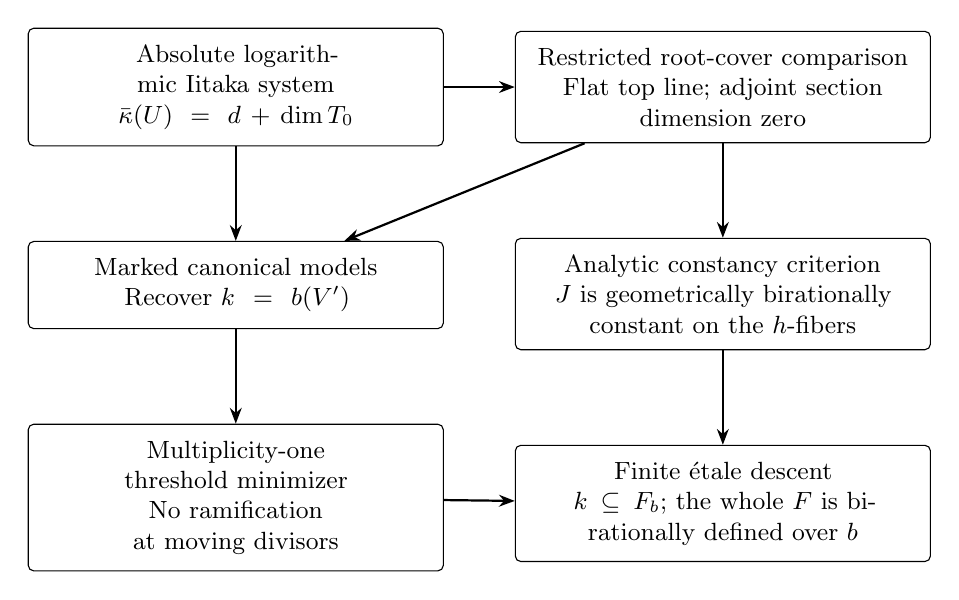
\begin{tikzpicture}[
  box/.style={draw,rounded corners=2pt,align=center,text width=.40\textwidth,
              inner sep=6pt,font=\small},
  arrow/.style={-{Stealth[length=2mm]},thick},node distance=12mm and 9mm]
\node[box] (parameter) {Absolute logarithmic Iitaka system\\
 $\kbar(U)=d+\dim T_0$};
\node[box,right=of parameter] (hodge) {Restricted root-cover comparison\\
 Flat top line; adjoint section\\dimension zero};
\node[box,below=of parameter] (marked) {Marked canonical models\\
 Recover $k=b(V')$};
\node[box,below=of hodge] (constant) {Analytic constancy criterion\\
 $J$ is geometrically birationally\\constant on the $h$-fibers};
\node[box,below=of marked] (cover) {Multiplicity-one threshold minimizer\\
 No ramification at moving divisors};
\node[box,below=of constant] (whole) {Finite \'etale descent\\
 $k\subseteq F_b$; the whole $F$ is birationally defined over $b$};
\draw[arrow] (parameter) -- (hodge);
\draw[arrow] (hodge) -- (constant);
\draw[arrow] (parameter) -- (marked);
\draw[arrow] (hodge) -- (marked);
\draw[arrow] (marked) -- (cover);
\draw[arrow] (cover) -- (whole);
\draw[arrow] (constant) -- (whole);
\end{tikzpicture}

\caption{The parameter field and the two constancy steps. The restricted
root-cover comparison supplies a flat line for analytic constancy and
a zero-dimensional adjoint section system for marked-model recovery.
The final field retains the relative Iitaka-base coordinates, giving
a bound for the variation of the whole $F$.}
\label{fig:whole-fiber-route}
\end{figure}

\subsection{Smooth families}

For smooth families, the good-model theorem of the companion
\emph{Log abundance in characteristic zero} and Taji's rigidity
theorems give a further application. This application is not used in
the proof of Theorem~\ref{thm:main}. A smooth quasi-projective base $V$ is
\emph{Campana-special} if, for any smooth projective compactification
$(Y,D)$ with reduced SNC boundary, every invertible subsheaf
$L\subseteq\Omega_Y^p(\log D)$ satisfies $\kappa(L)<p$ for
$1\leq p\leq\dim V$ \cite[\S1]{TajiGoodModels}.

\begin{corollary}[Variation and birational isotriviality]
\label{cor:nonuniruled-rigidity}
Let $f:U\to V$ be a smooth projective surjection with connected fibers
between smooth connected complex quasi-projective varieties. Assume
that every closed fiber is non-uniruled. Then
\[
\begin{aligned}
 \kbar(V)=-\infty&\quad\Longrightarrow\quad \Var(f)<\dim V,\\
 \kbar(V)\geq0&\quad\Longrightarrow\quad \Var(f)\leq\kbar(V).
\end{aligned}
\]
If $V$ is Campana-special, then $\Var(f)=0$. In particular, if
$\kbar(V)=0$, the family is birationally isotrivial.
\end{corollary}

\begin{proof}
Fix a closed fiber $F_v$. By \cite[Corollary~0.3]{BDPP}, its
non-uniruledness makes $K_{F_v}$ pseudo-effective. The companion
\cite[Corollary~11.2]{LogAbundanceCompanion} gives a normal projective
model $M_v$ with semiample $\Q$-Cartier $K_{M_v}$ and, on a common
smooth resolution $p:W\to F_v$, $q:W\to M_v$,
\[
 p^*K_{F_v}=q^*K_{M_v}+E,\qquad E\geq0
 \quad\text{and $E$ is $q$-exceptional}.
\]
For any prime divisor $P$ exceptional over $M_v$, pass to a higher
common resolution containing $P$ and denote the effective pullback
of $E$ again by $E$. Since $F_v$ is smooth, the discrepancy identity
\[
 a(P,M_v)=a(P,F_v)+\operatorname{coeff}_P E\geq0
\]
shows that $M_v$ has canonical singularities. Thus every $F_v$ admits
a good minimal model in the sense used by Taji. His variation is the
same whole-fiber field-of-definition invariant as
\eqref{eq:variation-definition}, so
\cite[Theorems~1.1--1.2]{TajiGoodModels} gives the dichotomy and the
special-base assertion. The case $\kbar(V)=0$ also follows from the
second inequality and $\Var(f)\geq0$.
\end{proof}

Here \emph{birationally isotrivial} means precisely $\Var(f)=0$.
No isomorphism or trivialization of the family, globally or after a
finite \'etale cover, is asserted.

For a smooth family in Theorem~\ref{thm:main} with $\kappa(F)\geq0$,
the nonnegative-base bound also follows directly from logarithmic
additivity \cite[Corollary~1.2]{AdditivityCompanion}. Choose compatible
smooth compactifications with $U=f^{-1}(V)$ and reduced complement
boundaries; their boundary strata are empty over $V$. The companion
gives $\kbar(U)=\kappa(F)+\kbar(V)$, where the geometric generic and
very general fiber Kodaira dimensions agree by generic base change and
upper semicontinuity in each pluricanonical degree. Comparing with
\eqref{eq:main} and cancelling the finite $\kappa(F)$ gives
$\Var(f)\leq\kbar(V)$. This comparison
does not address the negative-base branch or all special bases.

\subsection{Organization and an additional numerical result}

Section~\ref{it:section} constructs the parameter field, after stating
the exact logarithmic lower bound and the section conventions.
Section~\ref{sec:rankone} constructs the least-index root cover,
computes its parabolic line from actual relative orders, and proves
restricted flatness and finite character.
Section~\ref{cc:section} proves the analytic birational constancy
criterion, including contraction, equivariance and algebraic spreading.
Section~\ref{num:comparisons} develops the comparison for auxiliary
big model pairs at its first use. Section~\ref{sec:marking} uses
recognizable markings to recover the finite Iitaka-base normalization.
Section~\ref{ds:section} makes the cocycle constant, removes moving
ramification after every finite parameter extension, and identifies
the whole original function field. This completes the main theorem.

The final two sections give a separate extension. In
Section~\ref{num:second-base}, a nef contribution pulled back from an
adjoint-positive base replaces the Hodge line: interpolation retains
the full second Iitaka-base dimension. Its volume estimate bounds only
the effective action on the section image and is independent of the
degree of the auxiliary alteration. Section~\ref{ordinary:reductions}
applies that theorem to the ordinary relative Iitaka fibration and
recovers the same embedded parameter field. The exact reduced-root
and section-comparison inputs from the companion are stated there.
These sections are additional results; the logarithmic proof above
does not depend on them.

\section{The parameter field detected by logarithmic forms}
\label{sec:inputs}\label{it:section}

We first find a subfield of the original base field whose transcendence
degree is exactly the excess of the total logarithmic Kodaira dimension
over the fiber Kodaira dimension. This construction uses logarithmic
subadditivity and section maps; constancy of the fibers will be proved
after that field has been identified.

\subsection{The lower bound and section conventions}

The precise lower-bound input is the following companion theorem.
Only its projective form is used here. A compact manifold belongs to
Fujiki class $\mathcal C$ if it is bimeromorphic to a compact K\"ahler
manifold; in particular, every projective manifold belongs to this class.

\begin{theorem}[Reduced-SNC logarithmic subadditivity]
\label{spec:logarithmic}
Let $f:X\to Y$ be a surjective morphism with connected fibers between
smooth connected projective complex varieties. Let $D_X,D_Y$ be
reduced simple normal crossing divisors, with the zero divisor allowed,
such that
\[
 \operatorname{Supp}(f^*D_Y)\subseteq\operatorname{Supp}(D_X).
\]
For a very general fiber $F$, put $D_F=D_X|_F$. Then
\[
 \kappa(X,K_X+D_X)
 \geq\kappa(F,K_F+D_F)+\kappa(Y,K_Y+D_Y).
\]
The same assertion holds for compact manifolds in Fujiki class
$\mathcal C$ and holomorphic fibrations between them.
\end{theorem}

\begin{proof}
Apply
\cite[\PoneLog]{SubadditivityCompanion}.
The zero-divisor and $-\infty$ conventions here agree with that statement.
Only its projective form is used in the present paper.
\end{proof}

\subsection{Models, sections, and fields}

In the algebraic arguments below, varieties are integral unless a
finite splitting algebra is explicitly considered. For a surjective morphism with connected fibers between normal
varieties in characteristic zero, Stein factorization makes the base
field relatively algebraically closed in the total function field; the
generic field extension is regular and the generic fiber is geometrically
integral.
We use smooth projective resolutions of varieties and pairs
\cite{BierstoneMilmanFunctorial}; resolving the closure of a graph
also eliminates indeterminacy. Boundaries on these models will always
be specified. A rational section of a line bundle on a normal variety
is regular exactly when it is regular at every prime divisor.

\begin{lemma}[Exceptional section comparison]
\label{prelim:sections}\label{setup:log-modification}
Let \((X,\Delta)\) be a smooth pair with effective SNC rational boundary of coefficients at most one. Let \(\mu:X'\to X\) be a smooth log resolution, and let \(\Delta'\) be the strict transform of \(\Delta\) plus the reduced exceptional divisor. For every sufficiently divisible \(m\) and every line bundle \(A\) on \(X\), pullback and pushdown identify
\[
H^0\bigl(X,m(K_X+\Delta)+A\bigr)
\simeq
H^0\bigl(X',m(K_{X'}+\Delta')+\mu^*A\bigr).
\]
More precisely, there is an effective exceptional rational divisor $E$
with $K_{X'}+\Delta'=\mu^*(K_X+\Delta)+E$, and
\[
 \mu_*\cO_{X'}\bigl(m(K_{X'}+\Delta')\bigr)
   =\cO_X\bigl(m(K_X+\Delta)\bigr).
\]
This sheaf identity respects multiplication and remains valid after
pushing to any common base. More generally, adding an effective
exceptional divisor to a pulled-back rational divisor does not change
its divisible section spaces.
\end{lemma}

\begin{proof}
The discrepancy is exceptional because a birational morphism between
smooth varieties is an isomorphism at every generic target divisor.
For an exceptional prime $E_0$, choose boundary coordinates $z_i$ on
$X$, let $a_i=\ord_{E_0}(\mu^*z_i)$, and let $k_{E_0}$ be its
Jacobian order. Pulling back a logarithmic top wedge gives
$k_{E_0}+1\geq\sum_i a_i$: a nonzero wedge contains at most one
factor $du/u$ at $E_0=(u=0)$. If the boundary coefficients are
$\delta_i\leq1$, the discrepancy coefficient is therefore
\[
 k_{E_0}+1-\sum_i\delta_i a_i
       \geq\sum_i(1-\delta_i)a_i\geq0.
\]
Thus $E$ is effective. A rational function with poles only on an
effective exceptional divisor passes every codimension-one regularity
test on the normal target, so $\mu_*\cO_{X'}(mE)=\cO_X$.
The projection formula proves the sheaf and section identities,
including their twisted, relative, and multiplicative forms.
\end{proof}

The same comparison applies after restricting to a sufficiently general smooth fiber: the finitely many relevant horizontal strata meet it transversely, and vertical exceptional loci can be avoided. In particular, boundary changes on auxiliary higher models do not alter the original compact-fiber section dimension when only exceptional terms have been introduced on that fiber.

\begin{lemma}[Finite pullback]\label{num:finite}
If $\pi:V'\to V$ is a dominant generically finite morphism of normal
projective varieties and $D$ is a rational Cartier divisor on $V$, then
\[
 \kappa(V',\pi^*D)=\kappa(V,D).
\]
\end{lemma}

\begin{proof}
Stein factorization reduces to finite $\pi$, since a proper birational
morphism onto a normal variety has direct image $\mathcal O_V$.
Clear denominators. Each homogeneous section upstairs is integral over
the downstairs section ring: its monic characteristic polynomial in
the finite function-field extension has coefficients in the appropriate
powers of $D$. Trivializing $D$ at each prime of $V$ shows that these
coefficients are regular there, hence everywhere by normality. The
two graded rings therefore have the same transcendence degree. If the
downstairs ring has no positive-degree section, the norm excludes one
upstairs. These observations prove the assertion in all cases.
\end{proof}

\begin{lemma}[Fields, sections, and specialization]
\label{prelim:generic}\label{lem:field-transfer}
For a proper variety and a line bundle, global sections and their
multiplication maps commute with extension of the ground field.
Consequently Iitaka dimension is unchanged by field extension.
For a finite surjective morphism \(\pi:Y\to X\) of normal projective
varieties and a rational Cartier divisor \(L\) on \(X\),
\[
 \kappa(Y,\pi^*L)=\kappa(X,L).
\]
Finite collections of morphisms and birational identifications spread
over fields of finite type. Section-system statements on geometric
generic fibers may be checked on very general complex fibers,
simultaneously in countably many divisible degrees, and conversely.

If \(b\subseteq b'\) are algebraically closed fields and \(I\) is a
geometrically integral \(b\)-variety, every nonempty open subset of
\(I_{b'}\) contains a point of \(I(b)\).
\end{lemma}

\begin{proof}
Proper cohomology and flat base change identify the section spaces,
compatibly with multiplication, and hence preserve the dimensions of
the section maps. The finite-morphism assertion follows from Lemma~\ref{num:finite}. Morphisms, rational maps, and the identities making two
rational maps inverse use finitely many coefficients and spread after
finitely many denominators are inverted. On the smooth proper locus, in each fixed degree we shrink to an open
where the section dimension is constant; cohomology and base change
then identify the complete fiber space. Spreading the section maps
and excluding the countably many proper closed complements gives the
very-general-fiber assertion.

For the last assertion, work on an affine open of \(I\). A regular
function after extension to \(b'\) is a finite sum
\(\sum_j c_jf_j\), where the \(c_j\in b'\) are linearly independent
over \(b\) and \(f_j\in\cO(I)\). If it vanishes on every \(b\)-point,
then every \(f_j\) does too and is zero. Thus \(I(b)\) remains Zariski
dense after field extension, proving the assertion.
\end{proof}

\begin{lemma}[Upper addition and interpolation]\label{prelim:addition}
For a projective fibration \(u:T\to R\) and a rational divisor \(D\) with nonempty divisible section systems, the dimension of its section-system image is at most the dimension of \(R\) plus the dimension of the restricted section-system image on the generic fiber. In particular it is at most
\[
\dim R+\kappa(T_{\overline\eta},D|_{T_{\overline\eta}}).
\]
If \(D\) is rationally effective and \(b\geq1\) is rational, then for every rational divisor \(M\),
\[
\kappa(D+M)\geq\kappa(D+bM).
\]
\end{lemma}

\begin{proof}
For a sufficiently divisible system, compare its image with the base using the graph of the two rational maps. The fiber image has dimension bounded by the restricted complete system; the fiber dimension theorem gives the assertion, and taking the maximum over divisible systems proves the first inequality. This is the usual upper-addition estimate; see \cite[Theorem~4, p.~357]{IitakaOriginal}.

For the second claim use
\[
D+M=b^{-1}(D+bM)+(1-b^{-1})D.
\]
After clearing denominators, multiplication by a fixed effective section of the second summand embeds the corresponding section systems of the first. Their ratios are unchanged. Taking their image dimensions proves the assertion.
\end{proof}

We use the Iitaka fibration theorem for a divisor with nonnegative section dimension \cite[Theorems~3--4]{IitakaOriginal}: on a suitable smooth model its connected generic fiber has restricted divisor of Kodaira dimension zero, and the base has dimension equal to the original section dimension. Its application to a log adjoint divisor is explained in the two-base construction, including the comparison under subsequent resolutions.

For analytic computations, we normalize
\(\ddc=\frac{i}{2\pi}\partial\bar\partial\), so that
\(\ddc\log|s_D|^2=[D]\) in a local holomorphic frame. A weight is a local potential for a singular Hermitian metric; differences of weights on the same line bundle are globally defined functions. Smooth reference metrics are understood whenever a potential or a norm is compared globally. Positive universal normalization constants do not affect the integral estimates below.



Let $f:U\to V$ be the morphism in Theorem~\ref{thm:main}, and put
$d=\kappa(F)$.  If $d=-\infty$, the asserted inequality follows from the
convention for $-\infty$.  We therefore assume throughout this section that
$d\geq 0$.  We first obtain the contribution of $\kbar(V)$ and then construct
the bases used to control variation.  The subadditivity used in this section is
Theorem~\ref{spec:logarithmic}.

\subsection{Compactification and the first Iitaka base}

\begin{lemma}\label{it:compactification}
There are smooth connected projective compactifications $X$ and $Y$ of $U$
and $V$, respectively, and a surjective morphism $X\to Y$ with connected
fibers extending $f$, such that the reduced divisors
\[
 D_X=X\setminus U,\qquad D_Y=Y\setminus V
\]
have simple normal crossings and the inverse image of $V$ is exactly $U$.
In particular, $D_X$ has no component dominating $Y$, and
\begin{equation}\label{it:base-bound}
 \kappa(X,K_X+D_X)=\kbar(U)
 \geq d+\kbar(V).
\end{equation}
\end{lemma}

\begin{proof}
Take a smooth projective compactification of $V$ and resolve its boundary.
Since $f$ is projective, embed $U$ as a closed subscheme of a projective
space over $V$ and take its closure over the resulting projective base $Y$.
Equivalently, one can take the closure of the graph of $f$ in projective
compactifications.  Over $V$ this closure is already $U$: the original
family is proper over $V$, so no additional limit point is needed above
that open set.  Resolve the closure and its boundary, with all centers
outside the smooth open $U$.  Resolution and elimination of indeterminacy
in characteristic zero give the required morphism between smooth projective
varieties and the SNC boundary; see \cite{BierstoneMilmanFunctorial}.

The resulting morphism has a geometrically integral generic fiber.  Indeed,
the original proper morphism has connected fibers and normal base, so its
Stein factorization gives $f_*\cO_U=\cO_V$.  Thus $\C(V)$ is relatively
algebraically closed in $\C(U)$; in characteristic zero this extension is
regular.  The finite part of the Stein factorization of the compactified
morphism is consequently birational over $Y$, and hence is an isomorphism
because $Y$ is normal.  This proves connectedness of its fibers.

As $f^{-1}(V)=U$, every point of $D_X$ lies over $D_Y$, and
$\Supp(f^*D_Y)\subseteq\Supp(D_X)$.  A very general fiber lies over $V$,
has no boundary, and has ordinary Kodaira dimension $d$.
Theorem~\ref{spec:logarithmic} now applies to these smooth projective varieties,
connected fibers, and reduced SNC boundaries.  Its conclusion is
\eqref{it:base-bound}, by the compactification definition of logarithmic
Kodaira dimension.
\end{proof}

Fix, once and for all, a nonzero section
\begin{equation}\label{it:base-form}
 \xi\in H^0\bigl(Y,m(K_Y+D_Y)\bigr),\qquad m>0.
\end{equation}
Such a section exists because $\kbar(V)\geq0$.  It is essential here that
$\xi$ is logarithmic: no nonnegative ordinary Kodaira dimension of $Y$ is
assumed.

We recall the boundary convention for all subsequent source models.
If $\pi:X_1\to X$ is a smooth birational model, set
\[
 D_1=\pi_*^{-1}D_X+\operatorname{Exc}(\pi)_{\mathrm{red}}.
\]
The SNC discrepancy formula gives
\begin{equation}\label{it:exceptional-sections}
 K_{X_1}+D_1
 =\pi^*(K_X+D_X)+\sum_E A(E;X,D_X)E,
 \qquad A(E;X,D_X)\geq0,
\end{equation}
where the sum is exceptional.  For every positive integer $a$, divisorial
testing on the normal target therefore gives
\[
 \pi_*\cO_{X_1}\bigl(a(K_{X_1}+D_1)\bigr)
 =\cO_X\bigl(a(K_X+D_X)\bigr).
\]
Thus these modifications preserve the entire adjoint section ring, not
just its Iitaka dimension.  The same argument permits a pulled-back
rational twist in divisible degrees.  After each modification we resolve
the boundary again, using the same convention.

\begin{proposition}\label{it:diagram}
There are smooth connected projective varieties $X_*,X',W,Z$, a birational
morphism $X'\to X_*$, and morphisms
\[
 X'\xrightarrow{x}W\xrightarrow{g}Y,
 \qquad h:W\to Z,\qquad q=h\circ x,
\]
with the following properties.
\begin{enumerate}[label=\textup{(\roman*)}]
 \item The variety $X_*$ is a smooth model of $X$ carrying a resolved
 absolute Iitaka map for $K_X+D_X$.  Its boundary $D_*$, and the boundary
 $D'$ on $X'$, follow the strict-transform-plus-reduced-exceptional
 convention.  The map $q$ is the pullback of this Iitaka map, and
 \begin{equation}\label{it:iitaka-dimension}
  \dim Z=\kbar(U).
 \end{equation}
 \item The morphisms $x,g,h$ are surjective and have connected fibers and
 geometrically integral generic fibers.  The induced map from $W$ to
 its image in $Y\times Z$ is generically finite.  In particular,
 $W_z\to g(W_z)$ is generically finite for very general $z$.
 \item The divisor
 $D_W^0=(g^*D_Y)_{\mathrm{red}}$ is SNC.  On very general fibers over $Z$,
 all the relevant varieties and boundary strata are smooth, and
 \begin{equation}\label{it:absolute-fiber}
  \kappa\bigl(X_{*,z},K_{X_{*,z}}+D_*|_{X_{*,z}}\bigr)
  =\kappa\bigl(X'_z,K_{X'_z}+D'|_{X'_z}\bigr)=0.
 \end{equation}
\end{enumerate}
One may make further compatible smooth birational modifications, retaining
these assertions.  After the finite preparations in this section, $X_*$
can be fixed as an earlier model, and every subsequent source model is
taken to dominate it.
\end{proposition}

\begin{proof}
By \eqref{it:base-bound}, $K_X+D_X$ has nonnegative section dimension.
The divisor Iitaka theorem gives a resolved map with base dimension
$\kbar(U)$ and with restriction of the divisor having section dimension
zero on a very general fiber.  The needed statement is
\cite[Theorem~3, p.~357, and its proof in \S4, pp.~361--363]{IitakaOriginal}.
The stabilized section field is relatively algebraically closed in
$\C(X)$ by \cite[\S3, Proposition~1, p.~359]{IitakaOriginal}.  In the case
$\kbar(U)=0$, the map is the map to a point.

For clarity, the fiber conclusion concerns the full restricted section
system.  On a resolution, a sufficiently divisible system has moving part
pulled back from a big system on the Iitaka base.  In a divisible degree
there is consequently a section after subtracting a pulled-back ample
divisor.  Any extra independent plurisections on the generic fiber extend
after an ample pullback twist.  Multiplying by the preceding section
would then enlarge the stabilized section field, which is impossible.
Doing this in each degree gives the assertion on very general fibers.
Formula~\eqref{it:exceptional-sections} allows the theorem to be applied
to the log divisor on each higher source model itself.  Adjunction on a
smooth fiber identifies its restriction with that fiber's log canonical
divisor.  This proves \eqref{it:absolute-fiber}, including after further
compatible resolutions and birational changes of the Iitaka base.

Let $K=\C(X)$, $L_Y=\C(Y)$, and $L_Z=\C(Z)$, viewed as subfields of $K$.
The combined image in $Y\times Z$ has function field $L_YL_Z$.  Let $L_W$
be the relative algebraic closure of this compositum in $K$, a finite
extension of $L_YL_Z$.  Normalize the combined image in $L_W$, resolve it,
and resolve the resulting rational map from a higher source model.
These operations give the displayed morphisms.

The field $L_W$ is relatively algebraically closed in $K$ by construction.
Moreover, $L_Y$ and $L_Z$ are relatively algebraically closed in $K$, so
each is relatively algebraically closed in $L_W$.  In characteristic zero
the three corresponding generic field extensions are regular.  This
proves geometric integrality of the generic fibers of $x,g,h$; properness
and the normality of their targets give connectedness by Stein
factorization.  Finiteness of $L_W/(L_YL_Z)$ gives generic finiteness to
the combined image and hence generic finiteness of the indicated fiber
maps.

Finally resolve $D_W^0$ and the source boundary and lift all the maps.
Outside a proper closed subset of $Z$, the morphisms and every dominating
boundary stratum are smooth, and the nondominating strata are absent.
This follows from generic smoothness applied to the finitely many strata.
It gives the asserted very general SNC fiber data.  The section-ring and
field arguments just given are unchanged by these birational operations.
\end{proof}

The two maps just constructed are shown in
Figure~\ref{fig:combined-base}. The lower arrows in the figure are
the next objective; they will identify the required subfield of
$\C(Y)$.
\begin{figure}[ht]
\centering
\begin{tikzcd}[row sep=large,column sep=huge]
 & X' \arrow[d,"x"] & \\
 & W \arrow[dl,"g"'] \arrow[dr,"h"] & \\
Y \arrow[dr,dashed] & & Z \arrow[dl] \\
 & T_0 &
\end{tikzcd}
\caption{The two maps from the total space: $g x$ is the original
fibration and $h x$ is the absolute log Iitaka map. The construction
of $W$ makes its map to $Y\times Z$ generically finite onto its image. The proof
then constructs $T_0$ by parametrizing $g(W_z)$ and shows that both
base fields contain $\C(T_0)$. The lower arrows are conclusions of
the argument, not assumptions. Resolving the dashed map later
gives $S\to T_0$ with $S$ birational to $Y$.}
\label{fig:combined-base}
\end{figure}


\subsection{Logarithmic restrictions to the Iitaka fibers}

Write
\[
 n=\dim Y,\qquad r=\dim W_z,\qquad p_1=n-r.
\]
Generic finiteness of $W_z\to g(W_z)$ gives $0\leq r\leq n$, so
$p_1\geq0$.  The next argument explains how the logarithmic form on $Y$
produces a form of the correct degree on $W_z$.

\begin{lemma}\label{it:contraction}
For very general $z\in Z$, the form $\xi$ in \eqref{it:base-form} induces
nonzero sections of $m(K_{W_z}+D_W^0|_{W_z})$ by contraction with suitable
$p_1$ tangent directions at $z$.  In particular,
\[
 \kappa\bigl(W_z,K_{W_z}+D_W^0|_{W_z}\bigr)\geq0.
\]
\end{lemma}

\begin{proof}
Work over an open subset of $Z$ on which $h$ and all the boundary strata
are smooth.  On its inverse image the logarithmic cotangent sequence is
exact:
\[
 0\longrightarrow h^*\Omega_Z^1
 \longrightarrow\Omega_W^1(\log D_W^0)
 \longrightarrow\Omega_{W/Z}^1(\log D_W^0)
 \longrightarrow0.
\]
The last bundle has rank $r$.  Since $n=r+p_1$, the exterior-power
filtration has no term of base degree below $p_1$, and its first quotient
is the canonical map
\begin{equation}\label{it:wedge-quotient}
 \bigwedge^n\Omega_W^1(\log D_W^0)
 \longrightarrow
 h^*\!\bigwedge^{p_1}\Omega_Z^1
 \otimes\det\Omega_{W/Z}^1(\log D_W^0).
\end{equation}
Pullback of logarithmic differentials under $g$ is regular here: locally,
the pullback of an equation for $D_Y$ is a monomial in equations for
$D_W^0$ times a unit.  Thus $g^*\xi$ is a section of the $m$th tensor
power of the left side of \eqref{it:wedge-quotient}.  Apply the quotient
tensorwise and, on $W_z$, evaluate on any $p_1$ fixed vectors in $T_zZ$.
The result is a global section of
\[
 \bigl(\det\Omega_{W/Z}^1(\log D_W^0)|_{W_z}\bigr)^{\otimes m}
 \simeq\cO_{W_z}\bigl(m(K_{W_z}+D_W^0|_{W_z})\bigr).
\]
This construction is independent of local lifts of the chosen tangent
vectors: replacing one lift by a relative tangent vector inserts $r+1$
relative vectors into an alternating form, so contributes zero.  It is
therefore valid along the entire boundary of the fiber, rather than
only on its interior.

At a generic point of $W_z$, the differential of $g$ has rank $n$, while
its restriction to the tangent space of $W_z$ has rank $r$.  The induced
normal map from $T_zZ$ consequently has rank $p_1$.  Some choice of the
$p_1$ vectors gives a nonzero determinant, and hence a nonzero contracted
section.  When $p_1=0$, the same construction simply uses the relative
top-degree quotient, with no tangent vectors to choose.
\end{proof}

\begin{lemma}\label{it:zerofiber}
Let $J$ be the smooth geometric generic fiber of $x$, or a simultaneous
very general complex fiber.  Then
\begin{equation}\label{it:zero-equations}
 \kappa\bigl(W_z,K_{W_z}+D_W^0|_{W_z}\bigr)=0,
 \qquad
 \kappa(J)=\kappa\bigl(J,K_J+D'|_J\bigr)=0.
\end{equation}
The source-fiber equalities \eqref{it:absolute-fiber} hold on the same
very general locus.
\end{lemma}

\begin{proof}
First, $\kappa(J)\geq0$.  To see this using the ordinary canonical
divisor, take a very general compact $Y$-fiber of $X'\to Y$.  It is a
smooth birational model of the original fiber $F$ and therefore carries
a nonzero ordinary pluricanonical section because $d\geq0$.  The
restriction of this section to a general fiber of its map to $W_y$ is
nonzero: its zero divisor cannot contain all those fibers.  Adjunction
identifies this restriction, up to the one-dimensional determinant of
the base cotangent space, with an ordinary pluricanonical section on
$J$.  Since $D'|_J$ is effective, its log canonical divisor also has
nonnegative section dimension.

Now restrict $x$ to a very general fiber over $Z$:
\[
 x_z:(X'_z,D'|_{X'_z})\longrightarrow
       (W_z,D_W^0|_{W_z}).
\]
The source and base are smooth connected projective varieties, the
fibers are connected, and both displayed boundaries are reduced SNC.
Every component of the inverse base boundary is in the source boundary,
because both lie over $D_Y$. Thus Theorem~\ref{spec:logarithmic}
applies. Its conclusion, together with
\eqref{it:absolute-fiber} and Lemma~\ref{it:contraction}, is
\[
 0\geq
 \kappa\bigl(J,K_J+D'|_J\bigr)
 +\kappa\bigl(W_z,K_{W_z}+D_W^0|_{W_z}\bigr)\geq0.
\]
Both terms vanish.  The already proved ordinary nonnegativity, and
monotonicity under addition of an effective divisor, give
$\kappa(J)=0$ as well.  The simultaneous geometric-generic and very
general interpretations follow by base change in the countably many
section degrees.
\end{proof}

Although the original compactification has no horizontal boundary, a
later exceptional divisor can be horizontal for $x$.  Thus the proof
does not assert $D'|_J=0$; it proves both dimensions in
\eqref{it:zero-equations}.  On a very general $Y$-fiber, however, every
exceptional divisor that meets that fiber remains exceptional over the
original $F$: its center has codimension at least two after restriction,
by the dimension formula for a center dominating $Y$.  Accordingly,
\eqref{it:exceptional-sections} on this compact fiber identifies its
logarithmic section dimension with its ordinary dimension $d$.

\subsection{The image family and the second base}

\begin{proposition}\label{it:dimensions}
The models of Proposition~\ref{it:diagram} may be chosen together with
smooth connected projective varieties $S,T_0$ and morphisms in the
commutative diagram
\begin{equation}\label{it:full-diagram}
\begin{tikzcd}[column sep=large,row sep=large]
 X' \arrow[r,"x"] \arrow[rr,bend left=28,"q=h\circ x"]
 & W \arrow[r,"h"] \arrow[d,"g_S"] \arrow[dl,"g"']
 & Z \arrow[d]
 \\
 Y
 & S \arrow[l,"\rho"] \arrow[r]
 & T_0
\end{tikzcd}
\end{equation}
such that $\rho$ is birational, $g=\rho\circ g_S$, and
\begin{equation}\label{it:product-map}
 W\longrightarrow(S\times_{T_0}Z)_{\mathrm{main}}
 \quad\text{is dominant and generically finite}.
\end{equation}
Both $Z\to T_0$ and $S\to T_0$ have geometrically integral generic
fibers.  With $D_S=(\rho^*D_Y)_{\mathrm{red}}$ made SNC, one has
\begin{equation}\label{it:dimension-equations}
 \begin{gathered}
  \dim(W/Y)=d,\qquad
  \dim T_0=p_1,\qquad
  \dim Z=d+\dim T_0,\\
  \kappa\bigl(S_t,K_{S_t}+D_S|_{S_t}\bigr)\geq0
 \end{gathered}
\end{equation}
for very general $t\in T_0$.
\end{proposition}

\begin{proof}
\emph{The relative dimension over $Y$.}
The dimension of $W_y$ is the image dimension of the absolute Iitaka
coordinates restricted to a very general $Y$-fiber; the finite extension
in the definition of $W$ does not change this dimension.  Those
coordinates form a subsystem of a log pluricanonical system on that
fiber.  By the exceptional section comparison just explained, their
image dimension is at most $d$.  Conversely, upper addition for the
ordinary canonical divisor on that compact fiber, whose general fiber
over $W_y$ is $J$, gives
\[
 d\leq\dim W_y+\kappa(J)=\dim W_y.
\]
Here we use the upper addition inequality for section dimensions with
irreducible general fibers, as in \cite[Theorem~4, p.~357]{IitakaOriginal}; no
nonnegativity or subadditivity hypothesis on $W_y$ is involved.
Consequently $\dim(W/Y)=d$.

\emph{The differential of the image family.}
Let $C_z=g(W_z)\subseteq Y$ with its reduced structure.  The scheme
image of $W\to Y\times Z$ has geometrically integral generic fiber
over $Z$: its fiber function field lies between $\C(Z)$ and the
regular extension $\C(W)$.  Generic flatness, followed by restriction
to a smaller open, therefore yields a flat family of reduced integral
subschemes $C_z$ of $Y$. Hilbert representability
\cite[Theorems~3.1--3.2 and the discussion following Proposition~3.8]{GrothendieckHilbert}
therefore gives a parameter map
\[
 \tau:Z\dashrightarrow\operatorname{Hilb}(Y).
\]
We claim that the dimension of its image is exactly $p_1$.

Fix a very general $z$ and a basis of $T_zZ$.  Perform the contraction
in Lemma~\ref{it:contraction} for every $p_1$-tuple of basis vectors.
By Lemma~\ref{it:zerofiber}, all nonzero resulting sections in degree
$m$ are proportional.  Indeed, two independent sections in one degree
would give a nonconstant ratio and positive Iitaka dimension.

At a general smooth point $y\in C_z$, the normal deformation map is
\begin{equation}\label{it:normal-map}
 T_zZ\longrightarrow N_{C_z/Y,y}.
\end{equation}
It is computed by lifting a base direction to $W$, applying $dg$, and
taking its class modulo $T_yC_z$.  This is independent of the lift and
has rank $p_1$, since $g$ is dominant and $W_z\to C_z$ is generically
finite.  Locally trivialize the tangential determinant and the form
$\xi$.  Each contracted section is the $m$th power of the corresponding
$p_1$-minor of \eqref{it:normal-map}, multiplied by a common nonzero
factor.  Proportionality of the sections says that the $m$th powers of
all ratios of nonzero minors are constant as the point of $W_z$ varies.
The ratios themselves are constant: a rational function whose positive
power is constant is algebraic over $\C$, and hence is constant on an
integral complex variety.  The Pl\"ucker coordinates of
\eqref{it:normal-map} thus have constant ratios.  Its kernel, a subspace
of the fixed vector space $T_zZ$, is consequently independent of the
general point $y$.

To pass from this pointwise calculation to the parameter map, write
$\mathcal I_z$ for the ideal of $C_z$ in $Y$.  A Hilbert tangent vector
is a homomorphism
\[
 \mathcal I_z/\mathcal I_z^2\longrightarrow\cO_{C_z}.
\]
Such a homomorphism is zero if it is zero at the generic point: the
target is the structure sheaf of an integral scheme and has no
torsion.  On the general smooth locus of $C_z$, its normal value is
precisely \eqref{it:normal-map}.  It follows that $d\tau_z$ has the
same kernel as that normal map and therefore has rank $p_1$.  In
characteristic zero, generic differential rank equals the dimension
of the reduced image.  This proves the claim.

This argument includes the extremes.  If $p_1=0$, every $C_z$ has
dimension $\dim Y$ and is therefore $Y$, so the family is constant.
If $r=0$, the smooth connected $W_z$ is a point and its parameter
map has rank $\dim Y=p_1$.

\emph{Construction of $S$ and $T_0$.}
Let the function field of $T_0$ be the relative algebraic closure of
the image parameter field in $\C(Z)$, and take a smooth projective
model.  Then $\dim T_0=p_1$, and $Z\to T_0$ has geometrically
integral generic fiber.  Pull the universal image family back to
$T_0$ and take the component dominated by $W$, with a smooth
projective resolution denoted by $S$.  After compatible resolutions
all the maps in \eqref{it:full-diagram} are morphisms.  Its right
square commutes, and the induced map \eqref{it:product-map} is
dominant and generically finite: over a general $z$ it is the
generically finite map to the corresponding image member.

The generic fiber of $S\to T_0$ has dimension $r$.  Thus
$\dim S=r+p_1=\dim Y$, and its dominant map $\rho:S\to Y$ is
generically finite.  In fact it is birational.  The maps give the
field inclusions
\begin{equation}\label{it:field-tower}
 \C(Y)\subseteq\C(S)\subseteq\C(W)\subseteq\C(X).
\end{equation}
The first extension is algebraic, whereas $\C(Y)$ is relatively
algebraically closed in $\C(X)$.  Therefore $\C(S)=\C(Y)$.
In particular, the construction embeds $\C(T_0)$ in the original
base field $\C(Y)$.

For completeness, geometric integrality of the generic fiber of
$S\to T_0$ can be checked in the same field tower.  The field
$\C(T_0)$ is relatively algebraically closed in $\C(Z)$ by
construction, and $\C(Z)$ is relatively algebraically closed in
$\C(W)$.  It follows that $\C(T_0)$ is relatively algebraically
closed in $\C(W)$, and hence in its subfield $\C(S)$.  The
extension $\C(S)/\C(T_0)$ is therefore regular.  This also verifies
the geometric connectedness independently of the universal-family
description.

\emph{Dimensions and the logarithmic base fiber.}
The equality already proved over $Y$ gives
\[
 \dim W=\dim Y+d=\dim Z+r.
\]
Together with $\dim T_0=\dim Y-r$, this yields
$\dim Z=d+\dim T_0$.

Resolve the support of $D_S=(\rho^*D_Y)_{\mathrm{red}}$, lifting the
other maps once more.  Logarithmic pullback gives a nonzero section
$\rho^*\xi$ of $m(K_S+D_S)$.  Restrict it to a very general smooth
fiber $S_t$; this restriction is nonzero, since its zero divisor
cannot contain all fibers.  Adjunction, with the determinant of
$T_t^*T_0$ a constant one-dimensional factor, gives a nonzero
section of $m(K_{S_t}+D_S|_{S_t})$.  This proves the last assertion
of \eqref{it:dimension-equations}.  All these final resolutions
preserve the section and fiber properties in
Proposition~\ref{it:diagram}.  We now fix an earlier resolved
Iitaka source $X_*$ and take the common source $X'$ above it;
later source modifications will continue to dominate this fixed
model.
\end{proof}

\begin{remark}\label{it:constant-field-interface}
The field identifications in \eqref{it:field-tower} will also control
the constant field in the final descent.  Inside the prescribed
algebraic closure $\Omega$ of $\C(Y)$, set
$b=\overline{\C(T_0)}$.  The regular extensions
$\C(Y)/\C(T_0)$ and $\C(W)/\C(Y)$ remain regular after the
corresponding base changes.  Thus, if $I$ and $H_0$ are the
geometric generic fibers of $S$ and $W$ over $T_0$, their map
$H_0\to I$ has geometrically integral generic fiber.  Moreover,
$b(I)=b\C(Y)\subseteq\Omega$ is algebraic over $\C(Y)$, so
$\Omega$ is also an algebraic closure of $b(I)$.  These are
statements about the fields in the original diagram; they do not
assert constancy of the $x$-fiber or of the whole original fiber.
\end{remark}

\section{The root cover and its Hodge line}
\label{sec:rankone}\label{hd:section}

We retain the diagram and the boundary conventions of
Proposition~\ref{it:diagram}.  Thus
\[
 X'\xrightarrow{x}W,\qquad h:W\longrightarrow Z,
 \qquad q=hx,
\]
and $X'$ dominates a fixed earlier log Iitaka model $X_*$.  Its boundary
$D'$ is obtained from the boundary on $X_*$ by strict transform and addition
of the reduced exceptional divisor.  Put
$D_W^0=(g^*D_Y)_{\mathrm{red}}$.  Lemma~\ref{it:zerofiber} gives, for very
general $z\in Z$ and for the geometric generic fiber $J$ of $x$,
\begin{equation}
 \begin{split}
 \kappa(X_{*,z},K_{X_{*,z}}+D_*|_{X_{*,z}})&=0,\\
 \kappa(W_z,K_{W_z}+D_W^0|_{W_z})&=0,\\
 \kappa(J)=\kappa(J,K_J+D'|_J)&=0.
 \end{split}
 \label{ro:initial-zero}
\end{equation}
All subsequent modifications are smooth projective birational
modifications, with this same source-boundary convention.  We shall
construct an effective rational boundary $B$ and a nef rational Hodge line
$M$ on $W$, prove a section comparison on $W_z$, and then show that the
Hodge line is rationally trivial there.

\subsection{An ordinary cyclic cover}

\begin{lemma}[The root cover]
\label{ro:root}
Let $p$ be the least positive integer for which
$H^0(J,pK_J)\ne0$.  A generator $\omega_J$ determines a geometrically
connected cyclic cover of $J$.  Every smooth projective resolution
$\widetilde J$ of its finite normalization satisfies
\[
 \kappa(\widetilde J)=0,
 \qquad h^0(\widetilde J,mK_{\widetilde J})=1
 \quad\text{for every }m>0.
\]
The root form spans the entire ordinary top-form space.  After shrinking
a nonempty open $W^\circ\subset W$, these covers admit an equivariant
resolution forming a smooth projective family over $W^\circ$.
\end{lemma}

\begin{proof}
The spaces of pluricanonical sections commute with extension to an
algebraic closure of the ground field.  We first make that extension and
work with the smooth projective variety $J$ over an algebraically closed
field of characteristic zero.  Since $\kappa(J)=0$, every nonzero
pluricanonical system has dimension one.

Choose a rational canonical frame $\tau$ and write
$\omega_J=f\tau^p$.  Normalize $J$ in the field obtained by adjoining a
$p$th root of $f$.  This field extension has degree $p$.  Indeed, since the
ground field contains the $p$th roots of unity, reducibility of the Kummer
polynomial would make $f$ a $q$th power for some prime $q\mid p$.  If
$f=a^q$, then the rational $(p/q)$-canonical form
$a\tau^{p/q}$ has regular $q$th power.  Its order at every prime is
therefore nonnegative, so it is regular, contrary to the minimality of
$p$.  This also proves geometric connectedness before the extension of
the ground field.

Denote the finite normalization by $\pi_0:J^{\mathrm{nor}}\to J$ and a
smooth resolution by $\mu:\widetilde J\to J^{\mathrm{nor}}$.  The rational
root form $\eta$ on $\widetilde J$ satisfies
\begin{equation}
 \eta^{\otimes p}=(\pi_0\mu)^*\omega_J
 \label{ro:root-identity}
\end{equation}
as pluricanonical differentials.  Pullback of a regular pluricanonical
differential under a morphism of smooth varieties is regular.  Thus
\eqref{ro:root-identity} proves that $\eta$ is regular at every prime of
$\widetilde J$, including the resolution-exceptional primes.

Set $E=\operatorname{div}(\omega_J)$.  At a prime of $J^{\mathrm{nor}}$
over a prime of $J$ at which $E$ has coefficient $a\ge0$, let $e$ be the
ramification index.  The tame differential formula gives
\begin{equation}
 \ord(\eta)=\frac{ea}{p}+e-1.
 \label{ro:root-order}
\end{equation}
If $a=0$, adjoining the root of a unit is unramified at that prime and
$e=1$.  If $a\ge1$, the right side of \eqref{ro:root-order} is at most
$2ea$.  This bound is a statement at the primes of the finite
normalization; we do not assert it at every prime of its resolution.

For $s\in H^0(\widetilde J,mK_{\widetilde J})$, the rational function
$s/\eta^m$ consequently has poles at the primes of $J^{\mathrm{nor}}$
bounded by $2m\pi_0^*E$.  Normality therefore gives an injection
\begin{equation}
 H^0(\widetilde J,mK_{\widetilde J})
 \longrightarrow
 H^0(J^{\mathrm{nor}},\cO_{J^{\mathrm{nor}}}(2m\pi_0^*E)),
 \qquad s\longmapsto s/\eta^m.
 \label{ro:root-section-injection}
\end{equation}
Only codimension-one tests on $J^{\mathrm{nor}}$ enter this injection.

Lemma~\ref{num:finite} gives
$\kappa(J^{\mathrm{nor}},\pi_0^*E)=\kappa(J,E)=0$.
Since $\pi_0^*E$ is effective, each space on the right of
\eqref{ro:root-section-injection} has dimension one: two independent
sections would give a nonconstant section ratio. The nonzero section
$\eta^m$ gives the reverse inequality on the left, proving the assertion.

The integer $p$ and the one-dimensional generator space are unchanged
geometrically.  A rational generator can consequently be chosen as a
section of $pK_{X'/W}$.  The Kummer construction is algebraic over a
nonempty open of $W$.  An equivariant resolution of its projective
normalization, followed by shrinking the base and generic smoothness,
gives the asserted smooth projective family, with its fiberwise cyclic
deck action.
\end{proof}


\subsection{The entire top line and its extension}

A highest Hodge line means the
highest nonzero filtration piece $F^p$ of a pure variation, with
$F^{p+1}=0$ and $\rank F^p=1$. The rank condition concerns the entire
highest step; a rank-one eigenspace in a larger highest step does not
satisfy it. Its projective period map is the map on the connected universal cover
to the projective space of a flat reference vector space determined
by that line.
Its differential rank need not equal the rank of the full period map.
Our applications use rational polarizations and a monodromy-invariant
lattice in the rational local system. The full-period comparison in Theorem~\ref{period:adjoint} also
allows a real polarization, with a lattice in the underlying real local
system. The parabolic extension is the rational line obtained by making
boundary monodromy unipotent on local root covers, taking its canonical
Hodge extension, and descending with the resulting rational weights.
Finite-monodromy weights are retained in this convention.

\begin{lemma}[Parabolic extension]\label{hodge:extensions}
Let $P$ be smooth projective, let $D$ be a reduced SNC divisor, and let
$L^\circ$ be the highest line of a polarized integral pure variation
on $P\setminus D$. Its rational parabolic extension $L$ is nef.
This extension commutes with positive tensor powers and with pullback
by morphisms of smooth projective log pairs whose interiors map into
$P\setminus D$.
\end{lemma}

\begin{proof}
For unipotent local monodromy, the extension is the top filtration
subbundle of the Deligne--Schmid extension. Nefness and compatibility
with powers and log-pair pullbacks are
\cite[Lemmas~2.16 and~5.6]{BFMT}.
The pullback statement follows from functoriality of the unipotent
extension and the extended Hodge filtration.

Integral polarized monodromy is quasi-unipotent at the boundary.
In a crossing chart, take sufficiently divisible roots of the boundary
coordinates to make it unipotent. The resulting line is equivariant
for the finite deck group. A common positive power kills the
stabilizer characters on its fibers and descends to a line bundle in
the original chart. These descents agree on overlaps: compare them on
a common root cover and use uniqueness of the unipotent extension.
They define the rational parabolic line, including its finite-monodromy
weights. The same comparison proves compatibility with powers and
further log-pair pullbacks. This proves the quasi-unipotent assertions
by descent from the unipotent ones.

These comparisons can be made on a global smooth adapted alteration.
For example, a finite neat level of the integral monodromy, followed
by compactification and resolution, makes the boundary monodromies
unipotent. Extra boundary components on which the original variation
already extends have weight zero. The pullback of $L$ is the unipotent
extension there and is nef. Nefness descends under a proper surjective
map: every curve downstairs is dominated by a curve upstairs, and the
projection formula compares their degrees. Thus $L$ is nef.
\end{proof}

Fix the rational relative form $\omega_J$ of Lemma~\ref{ro:root}.  Enlarge
an SNC divisor on $W$ so that the root-cover family and its pure integral
polarized middle-cohomology variation are defined on its complement.
This enlargement specifies the domain of the variation; it does not
add logarithmic poles to the target section systems.

Let $\mathcal L$ be the highest nonzero Hodge filtration piece of the
middle-cohomology variation of the resolved root-cover family.
Lemma~\ref{ro:root} says that $\mathcal L$ has rank one.  Write $M$ for
its parabolic rational extension to the prepared SNC compactification
$W$.  Lemma~\ref{hodge:extensions} makes $M$ nef.

\subsection{Actual divisorial orders and the boundary}

Two divisorial tests enter the comparison. The first records which
poles a coefficient on $W$ may have while its product with the
relative pluriform remains logarithmic at every actual source
component. It gives a minimum over those components. The second
test ranges over divisorial valuations on all higher models; the
metric calculation below will identify it with an integrability
threshold. For each prime $P$ of $W$, we denote these two quantities
by $t_P$ and $\lambda_P$, respectively.

\begin{proposition}[Divisorial normalization]
\label{ro:divisors}
For a prime divisor $P$ on $W$, and for a prime divisor $Q$ on the actual
source $X'$ dominating $P$, set
\begin{equation}
 \begin{aligned}
 m_Q&=\ord_Q(x^*P),\qquad
 r_Q=\frac1p\ord_Q(\omega_J),\qquad
 d_Q=\operatorname{coeff}_Q(D'),\\
 t_P&=\min_{\substack{Q\mapsto P\\Q\text{ on }X'}}
                   \frac{r_Q+d_Q}{m_Q},\\
 \lambda_P&=\inf_{Q\mapsto P}\frac{1+r_Q}{m_Q},\qquad
 B_P=1-\lambda_P+t_P.
 \end{aligned}
 \label{ro:orders}
\end{equation}
In the definition of $\lambda_P$, $Q$ runs over divisorial valuations on all higher
smooth source models.  In both formulas $r_Q$ is measured in the actual
relative canonical bundle with respect to the smooth base $W$.

The two rational divisors
\[
 T=\sum_Pt_PP,
 \qquad B=\sum_PB_PP
\]
have finite support.  The divisor $B$ is an effective boundary and
\begin{equation}
 0\le B_P\le1,
 \qquad B\ge D_W^0=(g^*D_Y)_{\mathrm{red}}.
 \label{ro:boundary}
\end{equation}
The formulas at unchanged codimension-one base points are invariant
under further source resolutions with the prescribed boundary
convention.  They are also preserved, allowing splitting of components,
by an \'etale extension of the base DVR and the corresponding source
base change.  After a further birational preparation of $W$, $B$ can be
assumed to have SNC support.
\end{proposition}

\begin{proof}
At the generic point of $P$, correct the relative form by the factor
$u^{-pt_P}$, where $u$ is a local equation for $P$; take a tensor power to
make the exponent integral.  At every actual component over $P$ its
normalized order satisfies
\begin{equation}
 r_Q-m_Qt_P+d_Q\ge0.
 \label{ro:actual-test}
\end{equation}
Orders at divisors horizontal over $W$ are nonnegative, since
$\omega_J$ is an ordinary regular pluricanonical form on the generic
fiber.  Near the generic point of $P$, the corrected form is therefore a
logarithmic pluriform for the actual SNC pair $(X',D')$.

The discrepancy inequality for a reduced SNC pair says that pullback
to a higher smooth model is still logarithmic for strict transform plus
reduced exceptional boundary.  In particular, the normalized ordinary
order of the corrected form at any higher prime is at least $-1$.
It follows that
\[
 \frac{1+r_Q}{m_Q}\ge t_P
 \quad\text{for every }Q\mapsto P,
 \qquad\text{and hence}\qquad \lambda_P\ge t_P.
\]
If $Q$ attains the actual minimum defining $t_P$, then
\begin{equation}
 0\le\lambda_P-t_P
 \le \frac{1+r_Q}{m_Q}-\frac{r_Q+d_Q}{m_Q}
 =\frac{1-d_Q}{m_Q}\le1.
 \label{ro:boundary-inequalities}
\end{equation}
This proves $0\le B_P\le1$.  If $P$ is contained in $g^{-1}D_Y$, every
actual component over $P$ lies in $D'$ and has $d_Q=1$.  The middle term
of \eqref{ro:boundary-inequalities} is then zero, so $B_P=1$.

Resolve, over the generic point of $P$, the support of the form's zero
and pole divisor together with $x^*P$.  On this resolution the relevant
conditions are monomial inequalities.  The SNC discrepancy inequality
shows that inequalities at its components imply the inequalities on
every higher model.  Thus a finite log resolution computes $\lambda_P$;
in particular it is rational.  Outside a finite divisorial subset of
$W$, the fibers are smooth and integral, the relative form has no
vertical zero or pole, and there is no vertical source boundary.  There
the actual component has $m_Q=1$, $r_Q=d_Q=0$, and the smooth-fiber
calculation gives $t_P=0$ and $\lambda_P=1$.  This proves finite support.

On a further source resolution, the old actual divisors remain.  They
still attain the old minimum.  Equation~\eqref{ro:actual-test} holds at
every new actual divisor by logarithmic pullback, so the minimum cannot
decrease.  The all-valuation infimum is unchanged.  An \'etale base-DVR
extension preserves canonical frames up to units, multiplicities, and
all the displayed orders; the same assertion holds on a fixed log
resolution, including when a divisor splits.  Finally resolve the finite
support on the base, resolve the source map, and recompute
\eqref{ro:orders}.  All previously unchanged codimension-one points keep
their coefficients, and new support lies on the exceptional base
divisor.  The inequalities just proved apply to the recomputed data.
\end{proof}

\begin{corollary}[A zero boundary coefficient]
\label{ro:zero-boundary}
If an actual coefficient $B_P$ in Proposition~\ref{ro:divisors} is zero,
some actual source component $Q$ over $P$ satisfies
\begin{equation}
 d_Q=0,\qquad m_Q=1,\qquad
 \frac{1+r_Q}{m_Q}
   =\inf_{Q'\mapsto P}\frac{1+r_{Q'}}{m_{Q'}}.
 \label{ro:zero-minimizer}
\end{equation}
The same conclusion applies after the \'etale DVR extensions described
there.  It refers to the actual coefficient before any operation that
assigns a new reduced-exceptional boundary coefficient.
\end{corollary}

\begin{proof}
Take $Q$ attaining the first minimum in \eqref{ro:orders}.  The equality
$B_P=0$ makes $\lambda_P-t_P$ in
\eqref{ro:boundary-inequalities} equal to one.  Thus
\[
 1\le\frac{1-d_Q}{m_Q}\le1.
\]
Since $m_Q$ is a positive integer and $d_Q\in\{0,1\}$, this forces
$m_Q=1$ and $d_Q=0$.  Equality throughout also gives the final assertion
in \eqref{ro:zero-minimizer}.
\end{proof}

The component singled out by Corollary~\ref{ro:zero-boundary} will
enter the ramification argument in Sections~\ref{sec:marking}--\ref{ds:section}.
That argument uses both its multiplicity one and its attainment of
the all-valuation threshold. We first use the two order tests to
identify the Hodge line and compare sections.

\subsection{The metric identifies the Hodge contribution}

\begin{proposition}[The Hodge order]
\label{ro:metric}
At every prime $P$ of $W$, the parabolic order of the root form $\eta$ is
$\lambda_P-1$.  Consequently
\begin{equation}
 M\sim_{\Q}\sum_P(\lambda_P-1)P,
 \qquad
 T\sim_{\Q}B+M.
 \label{ro:metric-identity}
\end{equation}
\end{proposition}

\begin{proof}
On the smooth family locus, finite change of variables gives
\begin{equation}
 \|\eta_w\|_{\mathrm{Hdg}}^2
   =c_p\int_{J_w}|\omega_{J,w}|^{2/p},
 \label{ro:norm-fiber}
\end{equation}
where $c_p>0$ is constant and the expression on the right is the
canonical density associated with a pluricanonical form.  In a local
canonical frame, this density is the $2/p$ power of its coefficient
times the usual canonical volume density.

Take a general point of $P$, with base coordinates $(u,s_2,\ldots,s_l)$
and $P=(u=0)$.  Integrate \eqref{ro:norm-fiber} against base Lebesgue
measure and the factor $|u|^{-2\gamma}$.  Fubini and change of variables
reduce local integrability to an integral on a log resolution of the
total space.  The factors from the absolute canonical density and from
the base canonical frame cancel precisely as prescribed by
$K_{X'/W}=K_{X'}-x^*K_W$.  Thus, at a vertical prime $Q$, the monomial
exponent in the resulting density is
\[
 r_Q-\gamma m_Q.
\]
The transverse integral is finite exactly when
$r_Q-\gamma m_Q>-1$.  Horizontal primes have nonnegative ordinary order
and cause no further condition.  A finite SNC resolution computes all
these conditions, so the supremal integrability exponent is
\begin{equation}
 \sup\left\{\gamma:
 |u|^{-2\gamma}\|\eta\|_{\mathrm{Hdg}}^2\in L^1_{\mathrm{loc}}
 \right\}
 =\inf_{Q\mapsto P}\frac{1+r_Q}{m_Q}
 =\lambda_P.
 \label{ro:threshold}
\end{equation}
Here local integrability is measured against base Lebesgue measure.
The value at the endpoint itself is irrelevant to this supremum.

We compare this with the parabolic extension.  After a transverse root
coordinate killing the finite part of the monodromy, a nonvanishing
canonical extension frame has squared Hodge norm bounded above and
below by powers of $-\log|u|$.  This is the one-variable
nilpotent-orbit growth estimate for a polarized pure variation
\cite[\S\S4 and 6]{Schmid}.  Accordingly, a rational section of
parabolic order $a$ has squared norm
\[
 |u|^{2a}\,(-\log|u|)^{O(1)},
\]
where the notation means two-sided bounds by fixed powers of the
logarithm.  Its supremal exponent in \eqref{ro:threshold} is $1+a$.

There is a meromorphic coefficient to which this statement applies.
The form $\eta$ is an algebraic section of the top line on the
family locus.  One may use the regular-singular extension of the
geometric Gauss--Manin system.  Equivalently, the finiteness of the
threshold in \eqref{ro:threshold} gives a weighted $L^2$ bound for its
holomorphic coefficient in a nonvanishing extension frame.  Absorb the
logarithmic factors into an arbitrarily small power of the radius.  The
Laurent-series integral test then bounds the negative exponents of that
coefficient, excluding an essential singularity and proving meromorphic
extension.  The finite root coordinate gives a rational parabolic order
downstairs.  Clearing its denominator by a tensor power, and applying
the codimension-one extension test, gives the divisor of the rational
line $M$.

Comparing with \eqref{ro:threshold} proves $a=\lambda_P-1$.
There is no additional factor of $p$: the normalized order $r_Q$ already
contains $1/p$, and the density in \eqref{ro:norm-fiber} uses the same
normalization.  Finally
$t_P=B_P+(\lambda_P-1)$ at every prime, which proves
\eqref{ro:metric-identity}.  The transverse root coordinate has only
been used to compute the metric order; no section system has been
descended from a ramified alteration.
\end{proof}

\subsection{Preparation and transfer of sections}

We first record the birational preparation needed to avoid an
uncontrolled codimension-two image in a section comparison.

\begin{lemma}[Extracting source divisorial valuations]
\label{ro:extraction}
Let $T_*$ be a fixed smooth projective model of the source of a dominant
rational map to a smooth projective variety $R$.  After resolving the
map, making a birational modification of $R$, and resolving the source
again, we can arrange that every source divisor whose image in the new
base has codimension at least two is exceptional over $T_*$.  Further
smooth birational preparations of the base and compatible source
resolutions preserve this assertion.

If the maps also commute with maps to a fixed base $Z$, the same
assertion holds on their very general fibers over $Z$.
\end{lemma}

\begin{proof}
Resolve the rational map, obtaining a morphism $T_1\to R$.  Put
$e=\dim T_1-\dim R$.  A prime divisor of $T_1$ with image of codimension
at least two lies in the closed locus where the fiber dimension is at
least $e+1$.  There are only finitely many divisorial components in that
locus.  Consider those not exceptional over $T_*$.

For each such prime, its divisorial valuation $v$ on
$K=\C(T_1)$ has nontrivial restriction $w$ to $L=\C(R)$.  The latter is
a discrete rank-one valuation.  We justify that it is divisorial.
Residue elements algebraically independent over $\kappa(w)$ lift to
elements algebraically independent over $L$: in a proposed relation,
divide by a coefficient of least valuation and reduce to the residue
field.  Hence
\[
 \trdeg_{\kappa(w)}\kappa(v)\le\trdeg_LK.
\]
Since $v$ is divisorial, this gives
\[
 \trdeg_{\C}\kappa(w)
 \ge (\dim T_1-1)-(\dim T_1-\dim R)=\dim R-1.
\]
Conversely, lifts of algebraically independent residue elements for $w$,
together with an element of positive valuation, are algebraically
independent over $\C$.  Thus
$\trdeg_{\C}\kappa(w)\le\dim R-1$.  Equality follows.

Choose a residue transcendence basis and lift it to units of $L$,
together with an element generating the value group of $w$.  They give
a purely transcendental subfield of $L$ over which $L$ is finite.
Normalize the corresponding model in $L$ and take the center of $w$
above the DVR cut out by that positive-valuation parameter.  This
realizes $w$ as a prime divisor on a birational model of $R$.
Extract all the finitely many restrictions in this way and dominate the
result by a smooth projective model.  On a compatible smooth source
model, each of the original nonexceptional divisors now has divisorial
image.  Any new source prime is exceptional over $T_*$.  A further
birational base modification preserves the strict transform of each
extracted valuation divisor, proving persistence.

For the last assertion, shrink a nonempty open in $Z$ so that the
finitely many relevant loci, their images, and their boundary strata
have the expected fiber dimensions.  A prime divisor contracted to
codimension at least two on a fiber lies in the restriction of the
fixed excess-fiber-dimension locus.  A global component of codimension
at least two dominating $Z$ still has codimension at least two on a
general fiber.  Thus a divisorial component on a general source fiber
comes from a global divisorial component of that locus, possibly after
splitting.  Its image over $T_*$ has codimension at least two, and the
same dimension calculation makes its image exceptional on the general
fiber of $T_*$.  This proves the fiberwise assertion.
\end{proof}

\begin{proposition}[The Iitaka-fiber section bound]
\label{ro:transfer}
The models in Proposition~\ref{it:diagram} can be chosen, with the
divisors of Proposition~\ref{ro:divisors} recomputed on them, so that
\begin{equation}
 \kappa\bigl(W_z,K_{W_z}+B|_{W_z}+M|_{W_z}\bigr)\le0
 \label{ro:transfer-bound}
\end{equation}
for very general $z\in Z$.  The comparison is a comparison with the
section system on the fixed fiber $X_{*,z}$ in
\eqref{ro:initial-zero}.
\end{proposition}

\begin{proof}
Apply Lemma~\ref{ro:extraction} with fixed source $X_*$ and base $W$.
Retain the maps to $Y$ and $Z$, resolve the finite boundary supports,
and recompute \eqref{ro:orders}.  By the lemma, every divisor of a very
general fiber $X'_z$ whose image under $x_z$ has codimension at least two
is exceptional over $X_{*,z}$.

We also shrink the good open in $Z$ for the finitely many supports and
resolutions used in the divisorial calculation.  The tests defining $T$
then restrict to $W_z$.  To see this explicitly, over the smooth good
locus of $W$ those tests are zero.  Outside it, only restrictions of the
finitely many divisors dominating $Z$ can meet a general $W_z$ in a
divisor.  Generic smoothness and adjunction preserve the multiplicities
and relative-canonical orders there, with splitting of components
allowed.  Loci of higher codimension stay of higher codimension after
the shrinking just made.  The same reasoning on a fixed log resolution
computes all the higher-valuation inequalities.

Write $T_z=T|_{W_z}$.  For a sufficiently divisible integer $m$, take
\[
 \sigma\in H^0(W_z,m(K_{W_z}+T_z)).
\]
Using the relative canonical identification, multiply its pullback by
$\omega_J^{m/p}$.  This is a rational $m$-canonical form on $X'_z$.
If $Q$ is an actual source divisor with divisor image $P$, its normalized
order, after allowing the source boundary, is at least
\[
 m\bigl(r_Q-m_Qt_P+d_Q\bigr)\ge0
\]
by \eqref{ro:actual-test}.  A horizontal divisor passes the ordinary
test since the generic fiber generator is regular.  All other
untested divisors are exceptional over $X_{*,z}$.

Push the rational form to $X_{*,z}$.  At every prime of that smooth
fixed fiber, its strict transform has just passed the required
logarithmic test; hence the pushdown belongs to
\[
 H^0(X_{*,z},m(K_{X_{*,z}}+D_*|_{X_{*,z}})).
\]
Possible poles on a divisor exceptional over $X_{*,z}$ have no bearing
on this codimension-one test downstairs.  The construction is
injective.  More precisely, the common factor $\omega_J^{m/p}$ cancels
in ratios, so ratios of two input sections pull back by the dominant
map $x_z$ and their rational-map dimension is preserved.  The target
system has Iitaka dimension zero by \eqref{ro:initial-zero}.  The
identity $T_z\sim_{\Q}B|_{W_z}+M|_{W_z}$ from
Proposition~\ref{ro:metric} proves \eqref{ro:transfer-bound}.
\end{proof}

\subsection{Adjoint positivity for the restricted variation}

The section bound is now available on a very general $h$-fiber.
On that fiber, $K+B$ has a nonzero divisible section because
$B\geq D_W^0$. We shall use adjoint positivity to show that any
positive-dimensional adjoint base for the restricted Hodge line
would contradict the bound for $K+B+M$. The following is the
full companion input; its projective form follows immediately after.

\begin{theorem}[Full-period adjoint comparison]\label{period:adjoint}
Let $B$ be a smooth compact connected manifold in Fujiki class
$\mathcal C$, and let $B^\circ\subset B$ be a dense Zariski open
whose complement is an SNC divisor. Let $\mathbb V$ be a
real-polarizable pure variation of Hodge structures on $B^\circ$
with an integral lattice. Suppose a complex direct summand of
$\mathbb V_{\C}$ has a highest nonzero Hodge filtration step of rank
one, with rational parabolic extension $L$. There exist a modification
$\tau:B'\to B$, a connected-fiber surjective morphism $p:B'\to R$ to
a smooth projective variety, and a nef rational line bundle $A$ on
$R$ such that
\[
 \tau^*L=p^*A\quad\text{in }\operatorname{Pic}(B')\otimes\Q,
 \qquad K_R+cA\text{ is big for some }c\in\Q_{>0}.
\]
Positive rational rescaling of $L$ is allowed, and the line identity
persists under further modifications. A point is allowed for $R$;
then $\tau^*L$ is rationally trivial.
\end{theorem}

\begin{proof}
This is \cite[\PoneAdjoint]{SubadditivityCompanion},
whose proof uses the full period image and boundary numerical-rank
loss. The statement permits a complex summand of an integral ambient
variation; it is stronger in this respect than a theorem requiring
that summand itself to carry an integral lattice.
\end{proof}

\begin{proposition}[Projective adjoint comparison]\label{hd:adjoint}
Let $P$ be smooth connected projective, let $D$ be reduced SNC,
and let $L$ be the rational parabolic extension of the entire
highest Hodge line of a polarizable integral pure variation on
$P\setminus D$. There are a birational morphism
$\mu:P'\to P$ with $P'$ smooth projective, a surjective morphism
$a:P'\to R$ with connected fibers to a smooth projective variety,
and a nef rational line bundle $A$ on $R$ such that
\begin{equation}\label{hd:adjoint-conclusion}
 \mu^*L\sim_{\mathbf Q}a^*A,
 \qquad K_R+bA\text{ is big for all sufficiently large rational }b.
\end{equation}
The point quotient is allowed, in which case $\mu^*L$ is
rationally trivial.
\end{proposition}

\begin{proof}
The hypotheses meet Theorem~\ref{period:adjoint} directly. A projective
manifold belongs to class $\mathcal C$, a rational polarization
is a real polarization, and the entire complexification of the
given variation is a complex direct summand of itself. Its
highest nonzero filtration step is the specified rank-one line.
Thus the companion supplies $\tau:B'\to P$, $p:B'\to R$,
$A$ and $c>0$ with
\begin{equation}\label{direct:identity}
                \tau^*L\sim_{\mathbf Q}p^*A,
                \qquad K_R+cA\text{ big}.
\end{equation}

It remains to obtain a projective source model without changing
this identity or the connected-fiber property. The map
$P\dashrightarrow R$ induced by $p$ is meromorphic between
projective varieties and hence rational: its graph closure is
algebraic. Resolve that graph projectively to obtain a smooth
projective $P'$ and morphisms
\[
                       \mu:P'\to P,
                       \qquad a:P'\to R.
\]
On a common smooth modification of $B'$ and $P'$, the two maps
to $R$ agree. Pulling back \eqref{direct:identity} there therefore
identifies the pullbacks of $\mu^*L$ and $a^*A$.

Pullback by a proper birational morphism $v:T\to P'$ is
injective on rational line bundles. Indeed, if a line bundle
$N$ pulls back to a torsion line bundle, some positive power
$v^*N^m$ is trivial. Normality of $P'$ gives
$v_*\mathcal O_T=\mathcal O_{P'}$, and the projection formula
then gives $N^m\simeq\mathcal O_{P'}$. Applying this observation
to the common modification proves
\[
                          \mu^*L\sim_{\mathbf Q}a^*A.
\]

The generic fibers of $a$ are connected as well. The original
map $p$ has connected fibers and normal target, so
$\mathbf C(R)$ is relatively algebraically closed in
$\mathbf C(B')=\mathbf C(P)$. The same field extension occurs
for $a$. Its Stein factor is consequently finite birational
over the normal variety $R$, and hence is $R$ itself. Thus all
fibers of $a$ are connected.

Finally $A$ is nef. For every rational $b\geq c$,
$K_R+bA=(K_R+cA)+(b-c)A$ is big. If $R$ is a point, the line
identity already gives rational triviality; the zero-dimensional
bigness statement uses the usual point convention. This proves
the proposition.
\end{proof}

\begin{remark}\label{hd:further-models}
The conclusion is stable under further smooth projective
birational modification $\pi:R'\to R$ and a compatible
modification of the source.  The parabolic pullback property
preserves the line-bundle identity and nefness, while
\[
 K_{R'}+b\pi^*A
       =\pi^*(K_R+bA)+E_\pi,\qquad E_\pi\geq0,
\]
preserves bigness.  This is the form used when preparing the
later section comparisons.
\end{remark}

\subsection{Rational triviality on the Iitaka fiber}

The following weak-positivity consequence specifies the section
arithmetic used in the argument.

\begin{lemma}[Paying for a weak-positivity twist]
\label{ro:weak-addition}
Let $a:T_1\to R$ be a surjective morphism between smooth connected
projective varieties.  Let $\Delta$ be an effective rational SNC
boundary with coefficients in $[0,1]$, and let $N\sim_{\Q}a^*A$ for a
nef rational divisor $A$ on $R$.  Suppose
\[
 \kappa(T_1,K_{T_1}+\Delta)\ge0,
 \qquad K_R+cA\text{ is big}
\]
for a positive rational number $c$.  Then
\begin{equation}
 \kappa(T_1,K_{T_1}+\Delta+cN)\ge\dim R.
 \label{ro:weak-addition-bound}
\end{equation}
\end{lemma}

\begin{proof}
Use Lemma~\ref{ro:extraction} with fixed source $T_1$ and base $R$.
On the resulting smooth source $T_2$, let $\Delta_2$ be the strict
transform of $\Delta$ plus the reduced exceptional divisor, and pull
back $N$ and $A$; write $N_2=\pi^*N$ for the former pullback.
The SNC discrepancy inequality gives
\[
 K_{T_2}+\Delta_2
   =\pi^*(K_{T_1}+\Delta)+E_{\mathrm{exc}},
 \qquad E_{\mathrm{exc}}\ge0\text{ exceptional over }T_1.
\]
The section systems in the assertion therefore have the usual
pullback and pushdown comparison.  For a smooth birational base map
$\rho:R'\to R$,
\[
 K_{R'}+c\rho^*A
   =\rho^*(K_R+cA)+K_{R'/R}
\]
is still big, because $K_{R'/R}$ is effective.  Relabel the prepared
base as $R$, its divisor as $A$, and its source morphism as $a_2$.

Choose a sufficiently divisible positive integer $m$ for which the
relative direct image
\[
 \mathcal E_m
   =(a_2)_*\cO_{T_2}
          \bigl(m(K_{T_2/R}+\Delta_2)\bigr)
\]
has positive rank.  Such a choice is possible by restriction of a
nonzero section of a multiple of $K_{T_1}+\Delta$ to the generic fiber,
followed by pullback.  The pair $(T_2,\Delta_2)$ is log canonical,
$T_2$ is projective, and the base is smooth projective.  Thus
\cite[Theorem 1.1]{FujinoWeakPositivity} makes $\mathcal E_m$ weakly positive.

Put $L=K_R+cA$ and fix an ample integral divisor $H$ on $R$.  Increase
$m$ to clear the denominators needed below.  Since $L$ is big, choose a
positive integer $\alpha$ such that
\[
 \alpha mL-H\quad\text{is big}.
\]
The definition of weak positivity
\cite[Definition 7.2]{FujinoWeakPositivity} supplies a positive integer $\beta$ for
which
\begin{equation}
 \bigl(\operatorname{Sym}^{\alpha\beta}\mathcal E_m\bigr)^{**}
       \otimes\cO_R(\beta H)
 \quad\text{is generically generated by global sections}.
 \label{ro:weak-generation}
\end{equation}
At the generic point of $R$, multiplication of relative sections is
not the zero map: the power of any nonzero section on the integral
generic fiber is nonzero.  Generic generation in
\eqref{ro:weak-generation} therefore yields a global section whose
evaluation is a nonzero rational section $u$ of
\[
 \alpha\beta m(K_{T_2/R}+\Delta_2)+\beta a_2^*H.
\]
At every codimension-one point of $R$, the direct image is locally
free and the reflexive symmetric power agrees with its ordinary
symmetric power.  Evaluation is regular above those points.  Any
remaining pole divisor of $u$ thus has image of codimension at least
two and is exceptional over the fixed source $T_1$.

For a sufficiently divisible positive integer $q$, multiply $u^q$ by
the pullbacks of all sections of
\[
 q\beta(\alpha mL-H).
\]
The resulting rational sections lie in the class
\begin{align*}
 &q\alpha\beta m(K_{T_2/R}+\Delta_2)
       +q\beta a_2^*H
       +q\beta a_2^*(\alpha mL-H)\\
 &\hspace{25mm}
   =q\alpha\beta m(K_{T_2}+\Delta_2+cN_2).
\end{align*}
They are regular at every prime not exceptional over $T_1$, and so
push down to the required absolute section system on $T_1$.  Their
ratios are the pullbacks of the ratios of sections of the big divisor
$\alpha mL-H$.  These ratios give a rational map of dimension
$\dim R$, proving \eqref{ro:weak-addition-bound}.
\end{proof}

\begin{proposition}[Triviality on the Iitaka fiber]
\label{ro:trivial}
For very general $z\in Z$,
\begin{equation}
 M|_{W_z}\sim_{\Q}0,
 \qquad
 \kappa(W_z,K_{W_z}+B|_{W_z})=0.
 \label{ro:trivial-identities}
\end{equation}
These assertions also hold on the geometric generic $h$-fiber.
\end{proposition}

\begin{proof}
Set $T_1=W_z$, $\Delta=B|_{W_z}$, and $N=M|_{W_z}$. For the chosen
$z$, the fiber is smooth and all relevant boundary strata meet it
transversely, including those of the enlarged divisor defining the
domain of the variation. The log-pair pullback property in
Lemma~\ref{hodge:extensions} therefore identifies
$N$ with the parabolic extension of the restricted variation.
Moreover
\[
 \kappa(T_1,K_{T_1}+\Delta)\ge0
\]
by \eqref{ro:initial-zero} and $B\ge D_W^0$.  In particular,
$D=K_{T_1}+\Delta$ is rationally equivalent to an effective rational
divisor.

Apply Proposition~\ref{hd:adjoint} to the restricted integral polarized
variation whose \emph{entire} highest piece is this line. The comparison is applied directly to this restricted variation;
its entire complexification is an allowed summand in the companion theorem. On a higher smooth model it gives
\[
 N\sim_{\Q}a^*A,
 \qquad a:T_1\longrightarrow R,
 \qquad A\text{ nef},
 \qquad K_R+cA\text{ big for }c\gg1.
\]
On the higher source model use strict transform plus reduced
exceptional boundary for $\Delta$.  The logarithmic section comparison
preserves \eqref{ro:transfer-bound} and the rational effectivity of
$D$; the Hodge line is pulled back.  If $\dim R>0$, choose a sufficiently
large rational $c\ge1$.  Lemma~\ref{ro:weak-addition} gives
\[
 \kappa(T_1,D+cN)\ge\dim R>0.
\]
But
\begin{equation}
 D+N=\frac1c(D+cN)+\left(1-\frac1c\right)D.
 \label{ro:interpolation}
\end{equation}
After clearing denominators, multiplication by the section of the
effective last summand preserves rational-map dimensions.  Thus the
same positive lower bound holds for $D+N$, contradicting
\eqref{ro:transfer-bound}.  We conclude that $R$ is a point and
$N\sim_{\Q}0$.  Rational triviality descends through the intervening
birational morphisms, since their direct image of the structure sheaf
is the structure sheaf.  Now \eqref{ro:transfer-bound} and
$\kappa(D)\ge0$ give $\kappa(D)=0$.

Finally, these algebraic assertions pass to the geometric generic
fiber.  For the Kodaira dimension assertion, use generic base change
in the countably many divisible degrees.  For rational triviality,
choose an integer clearing the denominator of $M$.  For each positive
integer $j$, simultaneous nonvanishing of sections of the $j$th power
of that line and of its inverse is a closed condition on a smooth
proper family, and is equivalent to triviality on a connected
projective fiber.  The countable union of these loci contains every
very general $z$ by what we proved.  Hence some one of them contains a
dense open of $Z$; otherwise a very general point would avoid them
all.  Generic base change gives the required rational triviality on
the geometric generic fiber.
\end{proof}

\subsection{Flatness and finite character}

Rational triviality gives degree zero on every complete curve in an
Iitaka fiber. The curvature calculation below converts those zero
degrees into a flat highest line; finite character is then a statement
about the integral variation restricted to that algebraic locus.

\begin{corollary}[Degree zero on a curve]\label{hodge:degree-zero}
In Lemma~\ref{hodge:extensions}, suppose that $P$ is a smooth
projective curve. If $\deg L=0$, the projective highest-line map is
constant on the connected universal cover of $P\setminus D$.
Equivalently, $L^\circ$ is a flat line subbundle.
\end{corollary}

\begin{proof}
Pass to a finite cover making the boundary monodromies unipotent.
The extension pulls back, and its degree remains zero. Let $\alpha$
be the highest-line Hodge curvature. Griffiths' curvature formula
makes it semipositive and identifies its kernel with the kernel of
the projective line differential.

We check that its integral is the degree of the extension. For a smooth
reference curvature $\beta$, write $\alpha-\beta=\ddc u$. Near a
puncture, with $\rho=-\log|z|^2$, the Hodge norm and horizontal Schwarz
estimates give
\[
 |u|\le C(1+\log\rho),\qquad
 0\le\alpha\le C\frac{i\,dz\wedge d\bar z}{|z|^2\rho^2};
\]
see \cite[Theorem~5.1]{CK1989} and
\cite[Proposition~2.4 and Lemma~2.5]{BrunebarbeCadorel}.
Use products of cutoffs $\chi((\log\rho)/N)$, equal to one away
from a shrinking puncture neighborhood. Their second derivatives
are uniformly bounded in the cusp metric and supported on escaping
tails. Integration by parts bounds the error by the tail integral of
$(1+\log\rho)\rho^{-2}\,d\rho$, which tends to zero.
Thus $\int_{P\setminus D}\alpha=\deg L=0$. A continuous
nonnegative curvature form with zero integral vanishes. Its kernel
identity proves constancy on the cover and therefore on the original
universal cover.
\end{proof}

\begin{corollary}[Finite character of a line]\label{lem:finite-character}
Let $\mathbb V$ be a polarized integral variation of Hodge structures
on a connected smooth complex algebraic variety. Every rank-one
complex local subsystem of $\mathbb V_{\C}$ has finite monodromy.
\end{corollary}

\begin{proof}
Deligne's determinant theorem
\cite[Corollary~4.2.8(iii)(b)]{Deligne71} states that a positive tensor
power of the determinant of any complex local subsystem is trivial.
For a rank-one subsystem, the determinant is the subsystem itself.
Its character therefore takes values in a fixed finite group of roots
of unity. The theorem applies anew to the pulled-back variation on
any connected smooth algebraic locus.
\end{proof}

\begin{corollary}[Restriction and finite character]
\label{hodge:restricted-character}
Let $T$ be a connected smooth complex algebraic variety mapping into
the domain of a polarized integral pure variation whose entire highest
Hodge step is a line. If the pulled-back projective highest-line map is
constant, its highest line has finite monodromy character.
\end{corollary}
\begin{proof}
The pulled-back variation is again polarized, integral and pure.
Constancy of its projective highest line makes that line a rank-one
complex local subsystem. Apply Corollary~\ref{lem:finite-character}
to this restricted variation. No common exponent for different
algebraic loci is needed.
\end{proof}

\begin{corollary}[Flatness and finite character on the Iitaka fiber]
\label{ro:flat-character}
For very general $z\in Z$, the projective entire top line of the
restricted root-cover variation is constant on the connected good
locus of $W_z$, and its top-line character has finite image.
\end{corollary}

\begin{proof}
Put $T_1=W_z$ and $N=M|_{W_z}$. Proposition~\ref{ro:trivial}
gives $N\sim_{\Q}0$, and the pullback property in
Lemma~\ref{hodge:extensions} identifies $N$ with the parabolic
extension of the restricted entire top line.
The degree of $N$ on every complete smooth test curve is zero.
Corollary~\ref{hodge:degree-zero} makes the projective top line constant
along such curves.  Complete-intersection curves through general
points and tangent directions give projective constancy on the
connected good locus of $T_1$.
Corollary~\ref{hodge:restricted-character}, applied to this
restricted integral polarized variation, gives finite monodromy for
its original top line.
\end{proof}

\subsection{Alternative arguments for the Hodge line}
\label{ro:unitary-character}

\begin{remark}[Tensor comparison on restrictions]
The direct comparison above was applied to the restricted variation.
A separate integral tensor replacement, which makes
projective monodromy faithful, is proved in
\cite[\PfourTensor]{ProjectiveMethodsCompanion}; it gives the independent
adjoint comparison in \cite[\PfourAdjoint]{ProjectiveMethodsCompanion}.
On a connected algebraic restriction, that tensor construction must
be applied anew to the pulled-back integral variation. A replacement
faithful for the ambient moving line need not remain faithful after
restriction, so the monodromy and rational isotypic calculation must
be repeated on the restricted locus. Its positive tensor exponent may
depend on that locus; no common exponent is required. Thus it gives
an alternative adjoint comparison on each restriction. The proof here
uses the direct comparison and Corollary~\ref{hodge:restricted-character}.
\end{remark}

There is also a direct metric proof of the finite-character conclusion
in Corollary~\ref{ro:flat-character}. It uses the rational triviality
from Proposition~\ref{ro:trivial}, in addition to zero curvature.
Put $T_1=W_z$ and $N=M|_{W_z}$ on the prepared smooth
projective model. The constant projective top line on its connected
good open is a flat line. Its polarization, with the fixed Hodge sign,
is a positive flat metric, so its monodromy character $\chi$ is
unitary. Quasi-unipotence of the integral ambient variation makes
the characters around the finitely many SNC boundary components
roots of unity \cite{Schmid}.

Choose $e>0$ killing these local characters and clearing the
parabolic weights. Then $\chi^e$ extends across the boundary to
a unitary flat line on $T_1$; its holomorphic line bundle is the
parabolic tensor power $eN$. Since $N\sim_{\Q}0$, a further
positive tensor power is holomorphically trivial. For a nowhere-zero
holomorphic section of that power, the logarithm of its norm is
a globally defined pluriharmonic function. Compactness makes this
function constant. In a local flat unitary frame the section is
holomorphic of constant absolute value, hence constant, so it is
parallel. A positive power of $\chi$ is therefore trivial.
This recovers finiteness on this restricted locus without requiring
a common exponent for different loci.

\section{A birational constancy criterion}
\label{cc:section}

Section~\ref{sec:rankone} made the entire highest line flat, with
finite character, along the relevant Iitaka fibers. We now turn this
Hodge-theoretic information into birational constancy. The argument is
first carried out over a curve, where a single lifted vector field can
be analyzed, and then spread to arbitrary algebraic parameter loci.

\begin{theorem}[Birational constancy over a curve]
\label{cc:criterion}
Let $\pi^\circ:P^\circ\to C^\circ$ be a smooth projective morphism with
connected fibers, where $C^\circ$ is a smooth connected complex algebraic
curve.  Suppose that its very general fiber $D$ satisfies
\[
                 \kappa(D)=0,\qquad h^0(D,K_D)=1.
\]
Put $n=\dim D$ and assume that the entire top Hodge bundle
$F^n(R^n\pi^\circ_*\C\otimes\cO_{C^\circ})$ is a flat line with
finite monodromy character.  Then there are a finite
extension $L/\C(C^\circ)$ and a smooth connected projective variety
$D_0/\C$ such that the generic fiber after extension to $L$ is birational
to $(D_0)_L$.

If a finite group $\Gamma$ acts on $P^\circ$ over $C^\circ$, one can choose
$D_0$ with a $\Gamma$-action and choose this birational identification
$\Gamma$-equivariantly.  The same conclusion holds for a finite
fiberwise birational action, after replacing the family by an
equivariant smooth projective model.
\end{theorem}

The proof lifts a base direction to a meromorphic vector field on the
total space.  We first control this field along the zero divisor of a
global top form.  A singular-metric estimate then shows that every pole
is a fixed divisor of a small ample perturbation of the canonical
system.  Contracting those divisors makes the vector field regular;
its flow identifies nearby fibers.  Finite changes of the curve and
birational changes of the total space over a dense open do not change
the asserted conclusion.  A zero-dimensional connected smooth fiber is
a point, so throughout the construction we assume $n>0$.

In the log-smooth K\"ahler setting of Cao--Guenancia--P\u aun,
with klt boundary and numerically trivial fiberwise log-canonical
class, flatness of the pluricanonical direct image in its
Narasimhan--Simha metric implies analytic local triviality of the
pairs over the smooth locus
\cite[\S1.1, Theorem~1.2]{CaoGuenanciaPaun23}.
Here the flat line is the entire top Hodge line, with finite
character, and the fibers satisfy $\kappa(D)=0$ and $h^0(D,K_D)=1$.
The top form may have zeros, allowing poles in the lifted base
vector field; contracting its possible poles yields the birational
conclusion.

\subsection{A global form and its polarization}

\begin{lemma}
\label{cc:preparation}
After a finite change of the curve there are a smooth projective curve
$C$, a smooth projective variety $P$ of dimension $n+1$, and a projective
morphism $\pi:P\to C$ whose restriction over a nonempty open is
birational to the changed family, with the following properties.
There is a closed holomorphic $n$-form $\Theta$ on $P$ whose restriction
to each fiber over that open spans its ordinary top-form space.  Write
\[
 s\in H^0(P,K_{P/C}),\qquad \mathcal E=\operatorname{div}(s)
\]
for its relative canonical section and zero divisor.  The horizontal
part of $\mathcal E$ is relatively simple normal crossing over a smaller
open of $C$: the morphism and every horizontal zero-divisor stratum
are smooth there.  We call fibers over this open \emph{good fibers}.

One can choose an ample line bundle $H$ with a positive smooth metric,
whose curvature form is denoted by $h$, so that, for a positive area
class $\ell$ pulled back from $C$, there is a holomorphic $n$-form
$\alpha$ satisfying
\begin{equation}
           [h\wedge\Theta]=[\ell\wedge\alpha]
                  \quad\text{in }H^{n+1,1}(P).
\label{cc:pairing}
\end{equation}
In the equivariant case $P$ and $H$ can be chosen equivariant, $h$ is
invariant, and $\Theta$ transforms by the character of the fiber top
line.  Moreover, $P$ dominates a smooth projective model $P_0\to C$
with reduced fibers, and $\Theta$ is the pullback of a holomorphic form
on $P_0$.
\end{lemma}

Identity~\eqref{cc:pairing} has two uses: it removes the obstruction
to lifting the base vector field constructed below to $H$, and
later converts a weighted
integral on $P$ into an integral over good fibers. We obtain it by
choosing the global lift of the flat top form; that choice will leave
the relative form $s$ and its zero divisor unchanged.

\begin{proof}
Kill the finite character by a finite cover of $C^\circ$ and complete
the resulting curve.  Semistable reduction over a curve, followed by the
usual toroidal resolution, gives, after a further finite change, a smooth
projective model $P_0\to C$ with reduced fibers; see
\cite[Chapter II, semistable reduction over a curve]{KKMSD}.
Take a smooth projective common dominating model of this family and the
original changed family.  When $\Gamma$ is present, include the finitely
many translates in the graph construction and use an equivariant
resolution.  This also regularizes a finite birational action: take the
closure of the graph of all its maps in the product of their projective
models, on which the group permutes the factors, and resolve
equivariantly.  Over a dense smooth open, birational pullback preserves
ordinary top forms and is compatible with the cohomology local systems.
The chosen top class is therefore still invariant.

The flat generator already gives a relative top form on this smooth
open.  Choose a log resolution of its geometric generic zero divisor.
That resolution and its finitely many geometric components are defined
after a finite extension of the curve's function field.  Make this
change now and spread the resolution.  Repeat semistable preparation
at the boundary and take a smooth common dominating model, preserving
the chosen resolution over a dense open.  Thus the geometric divisor
components used below are defined before the final $P$, $H$, and
$\Theta$ are fixed.

The global invariant cycle theorem gives a surjection from the
cohomology of the smooth compactification onto the invariant part of
the fiber cohomology.  The restriction map is a morphism of Hodge
structures, so its strictness gives a preimage of the invariant
$(n,0)$-class in $H^{n,0}(P)$; these are precisely holomorphic $n$-forms.
Here we use \cite[Theorem~4.1.1(ii) and Corollary~4.1.2]{Deligne71}, with
smooth proper family over the good curve and smooth projective total
compactification.  Holomorphic forms on a smooth projective variety are
closed.

To describe the relative section, choose a local coordinate $t$ on $C$.
The absolute form $dt\wedge\Theta$, divided by the base frame $dt$,
defines $s$ in $K_{P/C}$.  These expressions agree under a change of
coordinate on the curve.  The section is holomorphic globally and is
nonzero on every good fiber.  Resolve its horizontal zero divisor and
shrink the good open so that the resulting horizontal components and
their intersections are smooth over the curve.  This gives the stated
relative normal crossings.  Any two lifts of the fixed flat top class
have the same restriction to every good fiber, and therefore give the
same relative section.  Thus the following change of lift does not alter
$s$ or this preparation of its zero divisor.

Put $V=H^0(P,\Omega_P^n)$ and let $N$ be the kernel of restriction to a
good fiber.  This kernel is independent of the chosen good fiber:
restriction of a global closed form gives a flat cohomology section, and
a holomorphic top form represents the zero cohomology class only when
it is zero.  Choose an ample $H$ and a positive metric, and set
\[
 B_h(\beta,\gamma)=\mathrm{i}^{n^2}
             \int_P h\wedge\beta\wedge\overline\gamma.
\]
This is a positive definite Hermitian pairing on $V$.  Indeed its
integrand is a positive multiple of the pointwise norm squared when
$\beta=\gamma$, and a nonzero holomorphic form is nonzero on an open
set.  For a positive smooth area form $\ell$ from the curve, the pairing
$B_\ell$ is semidefinite.  Fiber integration identifies its kernel with
$N$.  Consequently the image of the map
\[
       V\longrightarrow\overline V^{\,*},\qquad
       \beta\longmapsto B_\ell(\beta,-)
\]
is the annihilator of $N$.

Choose the lift $\Theta$ orthogonal to $N$ for $B_h$.  The functional
$B_h(\Theta,-)$ annihilates $N$, so it equals $B_\ell(\alpha,-)$ for
some $\alpha\in V$.  The duality pairing of $H^{n+1,1}(P)$ with
$H^{0,n}(P)$ is nondegenerate.  Applying it to the difference proves
\eqref{cc:pairing}.

In the equivariant case a tensor product of the translates of an ample
bundle admits a natural $\Gamma$-linearization; its metric can be made
invariant while keeping positive curvature.  Both $N$ and the pairing
are then invariant.  The unique orthogonal lift of the chosen top class
transforms by its top-line character.  The same character can be imposed
on $\alpha$ by projection to its character space.

Finally, a holomorphic form on a smooth projective birational model is
the pullback of a holomorphic form on every smooth projective model it
dominates.  Applying this to $P\to P_0$ gives the asserted descent of
$\Theta$.  A later positive tensor power of $H$ multiplies $h$ by a
positive integer and preserves all these conclusions, with $\alpha$
scaled accordingly.
\end{proof}

On the complement of the zeros and the critical locus, the kernel of
$\Theta$ is a holomorphic line transverse to the fibers.  On a good base
coordinate disk it has a unique generator $v$ satisfying
\begin{equation}
        d\pi(v)=\partial_t,\qquad \iota_v\Theta=0.
\label{cc:kernel}
\end{equation}
Here and below we use $\mathcal E$ for a divisor on the total space and
$E=\mathcal E|_D$ for its divisor on a good fiber.

\begin{lemma}[A meromorphic differential operator]
\label{cc:operator}
The vector field $v$ extends meromorphically to a neighborhood of each
general fiber, with poles bounded by $\mathcal E$.  After shrinking the
base disk, it is the symbol of a meromorphic first-order differential
operator $\nabla$ on $H$ with the same pole bound.
\end{lemma}

\begin{proof}
In a local relative canonical frame, write $\omega$ for the relative
$n$-form represented by $s$.  The normalization in
\eqref{cc:kernel} gives
\begin{equation}
                 \Theta=\iota_v(dt\wedge\omega).
\label{cc:contraction}
\end{equation}
Thus $sv$ is a holomorphic section of $T_P\otimes K_{P/C}$: contraction
with an absolute top form identifies this bundle, after choosing $dt$,
with $\Omega_P^n$.  Dividing by $s$ proves the pole bound.

Use the absolute scalar-symbol sequence
\begin{equation}
 0\longrightarrow\cO_P\longrightarrow\operatorname{At}(H)
                   \longrightarrow T_P\longrightarrow0.
\label{cc:atiyah}
\end{equation}
Its middle sheaf consists of first-order differential operators on $H$
with scalar symbol.  Its extension class is $c_1(H)$, up to the fixed
normalizing constant; this is the connection obstruction of
\cite{Atiyah57}.  For the specific assertion needed here, take frames
$e_i=g_{ij}e_j$.  Local lifts of the same vector symbol differ by its
contraction with $d\log g_{ij}$.  This is the cocycle representing the
stated extension class.

Tensor \eqref{cc:atiyah} by $K_{P/C}$.  The obstruction to lifting $sv$
is its contraction with $c_1(H)$ in $H^1(K_{P/C})$ on the neighborhood
in question.  In Dolbeault notation and using
\eqref{cc:contraction}, its restriction to $D_t$ is, up to a nonzero
constant and sign, the class obtained from $h\wedge\Theta$ by dividing
its top holomorphic degree by $dt$ and restricting to $D_t$.
This operation respects Dolbeault coboundaries.  In fact the total space
has dimension $n+1$, so a primitive of type $(n+1,0)$ necessarily contains
$dt$ in submersion coordinates; division by $dt$ commutes with
$\bar\partial$ before restriction.  Equivalently this is the canonical
restriction $K_P|_{D_t}\simeq K_{D_t}\otimes T_t^*C$ with a base frame
chosen.

The right side of \eqref{cc:pairing} gives zero under this operation:
a smooth area representative of $\ell$ contains $d\bar t$.  Hence the
fiber obstruction is zero for every good $t$.  Shrink to a Stein disk on
which cohomology and base change hold for $K_{P/C}$.  Leray and the
vanishing of higher coherent cohomology on the disk identify the
obstruction with a section of $R^1\pi_*K_{P/C}$.  It is zero because its
fiber values are zero.  Therefore $sv$ lifts to a holomorphic section of
$\operatorname{At}(H)\otimes K_{P/C}$ on the whole neighborhood.
Dividing this lift by $s$ produces $\nabla$, with the claimed symbol and
pole bound.  Replacing $H$ by a tensor power uses the induced operator
and leaves its symbol and its pole bound unchanged.
\end{proof}

\subsection{Vanishing on the zero divisor}

The lifted field may have poles along $\mathcal E$.  We first prove
that the absolute form vanishes on every component of this divisor.
This will make its pairing with every positive curvature current of
$K_{P/C}$ vanish, and supply the integral estimate used below.

\begin{lemma}
\label{cc:zeros}
The pullback of $\Theta$ to a resolution of every irreducible component
of $\mathcal E$ is zero.
\end{lemma}

\begin{proof}
We first treat a horizontal component.  Choose a simultaneous very
general good fiber $D$, so that all its positive pluricanonical section
spaces have dimension one.  Write
\begin{equation}
 E=\sum_j e_jD_j,\qquad R_0=E+E_{\mathrm{red}},\qquad
 S=D_i,\qquad B'=\sum_{j\ne i}D_j.
\label{cc:zero-data}
\end{equation}
The coefficients $e_j$ are positive integers, $E\sim K_D$, and the
support is simple normal crossing.  The components extend relatively
over a small disk.  In the local computations we use the same letters
for these relative extensions and their local equations.

The contradiction will take place in the section spaces of $R_0$.
Since
\[
                   E\le R_0\le2E,\qquad E\sim K_D,
\]
for every positive integer $m$ we have
\[
       1\le h^0(D,mR_0)\le h^0(D,2mE)
                              =h^0(D,2mK_D)=1.
\]
Thus every section of $mR_0$ is a multiple of its divisor section
and vanishes on $S$. We will construct a section whose restriction
to $S$ is nonzero.

Suppose that the restriction of $\Theta$ to the horizontal component
through $S$ is nonzero.  Let $z$ and $G$ be local equations for $S$ and
$R_0$, and put
\[
                   W=Gv,\qquad u=(W(z)/z)|_S.
\]
The pole bound in Lemma~\ref{cc:operator} shows that $W$ is holomorphic
and vanishes on the reduced zero divisor.  It is consequently
logarithmic along that divisor, so that both $W(z)/z$ and $W(G)/G$ are
holomorphic.  Under changes of the equations, $u$ transforms as a
section of $R_0|_S$.  Formula \eqref{cc:contraction} identifies its
nonvanishing at the general point of $S$ with the supposed nonvanishing
of $\Theta$ on the relative component.  Thus
\begin{equation}
                0\ne u\in H^0(S,\cO_S(R_0)).
\label{cc:u}
\end{equation}
Moreover $u$ is divisible by the full reduced divisor $B'|_S$.  To see
this at a crossing, the coefficients of $sv$ are holomorphic, while
$G/s$ has one factor for each component of $E_{\mathrm{red}}$.
Division by $z$ removes the factor belonging to $S$ and leaves all
other reduced factors.

Write the operator in a regular frame of $H$ as $\nabla=v+c$.  Its pole
bound also gives $Gc|_S=0$.  Replace $H$ by a sufficiently high tensor
power.  Relative generation supplies finitely many sections
$a_\lambda$ on a neighborhood of the whole fiber, vanishing on the
relative $S$, such that $a_\lambda/z$ generate $H(-S)$ along $S$.
For each $\lambda$ set
\[
 q_{k,\lambda}=\frac{\nabla^k a_\lambda}{k!},\qquad
 b_{k,\lambda}=\frac{G^k\nabla^ka_\lambda}{z}.
\]
The following recurrence proves in particular that the second
expression is holomorphic:
\begin{align}
 b_{k+1,\lambda}
  &=W(b_{k,\lambda})+
     \left(\frac{W(z)}z-k\frac{W(G)}G+Gc\right)b_{k,\lambda},
                                                       \label{cc:recurrence}\\
 b_{k,\lambda}|_S
  &=u^k(a_\lambda/z)|_S
           \prod_{j=0}^{k-1}\bigl(1-j(e_i+1)\bigr).
                                                       \label{cc:leading}
\end{align}
For the second equality, $W$ vanishes on $S$, $Gc|_S=0$, and
$(W(G)/G)|_S=(e_i+1)u$.  The other components of $G$ contribute zero
on $S$; this can be checked away from their intersections and then
extended holomorphically.  These facts prove both formulas by induction.
They also show that the restrictions of $q_{k,\lambda}$ are sections of
$\cO_D(kR_0+H-S)$. More explicitly, in a local frame of $H$,
\[
 q_{k,\lambda}=\frac{z}{G^k}\frac{b_{k,\lambda}}{k!}.
\]
The meromorphic expression on the left is therefore a holomorphic
section of the indicated twisted bundle, with local coefficient
$b_{k,\lambda}/k!$.

We need estimates as $k$ tends to infinity.  Cover a compact
neighborhood of $D$ by finitely many pairs of nested coordinate charts.
For a fixed $k$, divide each nesting margin into $k$ equal parts.  On
these charts the coefficients of $W$, $W(z)/z$, $W(G)/G$, and $Gc$ are
bounded.  At the $j$th step of \eqref{cc:recurrence}, Cauchy's estimate
for the derivative costs at most a constant times $k$, and the
zeroth-order coefficient costs at most a constant times $1+j\le k+1$.
It follows that the holomorphic coefficients $b_{k,\lambda}/k!$, in
smooth metrics for $kR_0+H-S$, are bounded by
\begin{equation}
                   \frac{(Ck)^k}{k!}\le C_1^k.
\label{cc:cauchy}
\end{equation}
This is a bound in the indicated twisted bundle, including across the
zero divisor.

Put $a=e_i+1\ge2$.  No factor in \eqref{cc:leading} is zero, and
\[
 \lim_{k\to\infty}
 \left|\frac{\prod_{j=0}^{k-1}(1-ja)}{k!}\right|^{1/k}=a>0;
\]
for example, the ratio of successive absolute values tends to $a$.
On $D$, take the weights
\[
 \frac1k\log\sum_\lambda
       \left|\frac{b_{k,\lambda}}{k!}\right|^2
       -\frac1k\varphi_{H-S},
\]
where $\varphi_{H-S}$ is a smooth weight on $H-S$ in the same
local frames. They are weights on $R_0$ with curvature loss tending
to zero and uniform upper bounds by \eqref{cc:cauchy}.  Their
regularized upper limit is a semipositive singular weight.  Formula
\eqref{cc:leading}, together with generation of $H(-S)|_S$, gives its
restriction a lower bound by $\log|u|^2$ up to a constant.  Finally take
the maximum with the divisor weight of $R_0$.  We obtain a semipositive
weight $\varphi$ on $R_0$ satisfying
\begin{equation}
      \varphi\ge\log|s_{R_0}|^2,\qquad
      \varphi|_S\ge\log|u|^2-C.
\label{cc:weight-bounds}
\end{equation}
All weights here are written in compatible local frames; the
inequalities are invariant statements about the corresponding metrics.

We now extend a nonzero power of $u$ using
\cite[Theorem~4.1, conditions~(19)--(23)]{DHP13}.  We record every
hypothesis in this application.  The ambient manifold is the smooth
projective $D$, and its smooth hypersurface is $S$.  For any integer
$m\ge2$ put
\begin{equation}
 \begin{split}
  F'&=mR_0-(K_D+S)\sim (m-1)R_0+B',\\
  \varphi_{F'}&=(m-1)\varphi+\log|s_{B'}|^2,\\
  A_0&=R_0-aS=\sum_{j\ne i}(e_j+1)D_j,\\
  \varphi_S&=1+\frac{\varphi-\log|s_{A_0}|^2}{a}.
 \end{split}
\label{cc:extension-weights}
\end{equation}
The first line uses $K_D\sim E$ and
$E_{\mathrm{red}}=S+B'$.  Thus $F'$ is an actual line bundle with the
indicated weight, after the indicated line-bundle identification.

Condition (19) of the extension theorem holds with its constant equal
to one, since \eqref{cc:weight-bounds} implies
\[
                  |s_S|^2e^{-\varphi_S}\le e^{-1}.
\]
For condition (20), the weights $1+\varphi/a$ and
$a^{-1}\log|s_{A_0}|^2$ are semipositive weights on rational line
bundles and have difference $\varphi_S$.  If integral bundles are used,
choose an integral $G_2$ sufficiently ample that $G_2-A_0/a$ has a
positive smooth rational-bundle metric, and add this metric to both
weights.  The difference is unchanged and both underlying bundles
become integral.

For condition (21), let $T_R=\ddc\varphi$.  Directly,
\begin{equation}
 \begin{split}
 \ddc\varphi_{F'}&=(m-1)T_R+[B']\ge0,\\
 \ddc\varphi_{F'}-\ddc\varphi_S
       &=\left(m-1-\frac1a\right)T_R+[B']+\frac1a[A_0]\ge0.
 \end{split}
\label{cc:extension-curvature}
\end{equation}
Here $a\ge2$ and $m\ge2$.  For condition (22), choose a positive
number
\[
  \varepsilon_0\le
       \min\left\{1,\min_{j\ne i}\frac{a}{e_j+1}\right\},
\]
omitting the inner minimum if there are no other components.  The
weight $\varphi$ is locally bounded above.  After normalizing local
defining functions to have norm at most one, each coefficient of
$\log|s_{B'}|^2$ is at least the corresponding coefficient in
$\varepsilon_0 a^{-1}\log|s_{A_0}|^2$.  Therefore
\[
       \varphi_{F'}\le
             \frac{\varepsilon_0}{a}\log|s_{A_0}|^2+C.
\]
A common smooth metric added to the two weights above changes this
inequality only by a bounded local term.  This proves precisely the
required domination of the subtracted weight's singularities.

The section to extend is
\[
       u^m\in H^0\bigl(S,\cO_S(mR_0)\bigr)
             =H^0\bigl(S,K_S+F'|_S\bigr).
\]
The lower bound for $\varphi|_S$ and $u\ne0$ also ensure that
the restricted weights are not identically minus infinity.
Condition (23) follows from the second bound in
\eqref{cc:weight-bounds}:
\begin{equation}
 |u|^{2m}e^{-\varphi_{F'}|_S}
                \le C\frac{|u|^2}{|s_{B'}|_S|^2}.
\label{cc:extension-integral}
\end{equation}
The quotient on the right is locally bounded because $u$ is divisible
by the full reduced divisor $B'|_S$.  There is in fact integrability
with a slightly larger weight exponent.  Writing $u=s_{B'}w$, the
density with exponent $1+\delta$ on $\varphi_{F'}$ is bounded by
\[
 C|s_{B'}|^{-2m\delta}|w|^{2-2(m-1)\delta}.
\]
It is integrable for $0<\delta<1/m$, by the normal crossings of
$B'|_S$ and the positive exponent on $|w|$.  This argument requires no
normal-crossing assertion about the other zeros of $w$.

The extension theorem now gives a section of $mR_0$ with restriction
$u^m\ne0$, contradicting the one-dimensionality of this section
space established above: its divisor section vanishes on $S$.
This proves the horizontal vanishing.

For vertical components, use the reduced-fiber model $P_0\to C$ in
Lemma~\ref{cc:preparation}, to which $\Theta$ descends.  At a general
point of a reduced fiber component the map has local equation $t=z$.
There the vanishing of the relative coefficient $s$ is exactly the
vanishing of the restriction of $\Theta$ to that component.  Every
vertical component on $P$ which is not exceptional over $P_0$ is tested
at the same generic point.  An exceptional divisor maps into a subset
of $P_0$ of dimension at most $n-1$, and the pullback of an $n$-form to
its resolution is zero.  These observations prove the remaining
vanishing assertions.  They also explain why the reduced-fiber model
is used: for $t=z^r$ with $r>1$, an additional differential factor
$z^{r-1}$ would not itself imply vanishing of the absolute form.
\end{proof}

\subsection{Curvature pairing and an integrability estimate}

We have proved that $\Theta$ vanishes on every component of
$\mathcal E=\operatorname{div}(s)$. Put
$\mu=i^{n^2}\Theta\wedge\overline\Theta$.
The resulting identity $[\mathcal E]\wedge\mu=0$ will control
singular metrics on $K_{P/C}$, and hence the poles of the normalized
kernel field $v$.

For a semipositive weight $T$ on $K_{P/C}$, the curvature pairing
with $\mu$ has the same integral as $[\mathcal E]\wedge\mu$ and
therefore vanishes. When $T\geq\log|s|^2$, applying this observation
to truncations shows that $\psi=T-\log|s|^2$ is constant along
almost every local kernel leaf. This permits the weighted use of
\eqref{cc:pairing} and gives an integrability exponent strictly
greater than one. We prove the estimate for arbitrary $T$ before
constructing the weight supplied by pluricanonical section spaces.

We use weights for metrics written as \(e^{-\varphi}\), and the convention
\[
 \ddc=\frac{i}{2\pi}\partial\bar\partial,
 \qquad \ddc\log|z|^2=[z=0].
\]
In particular, if \(\varphi_H\) is a local weight for the metric on
\(H\), then \(\ddc\varphi_H=h\).  Expressions such as
\(\log|s|^2\) below denote local weights in holomorphic frames; the
difference of two weights on the same bundle is a globally defined
function wherever both are finite.

\begin{lemma}\label{ca:integrability}
Let \(T\) be a semipositive singular weight on \(K_{P/C}\) such that
\(T\geq\log|s|^2\), and put
\(\psi=T-\log|s|^2\geq0\) off \(\mathcal E\).
There exists \(\delta>0\) such that
\begin{equation}\label{ca:global-integral}
 \int_P e^{(1+\delta)\psi}
       i^{n^2}h\wedge\Theta\wedge\overline\Theta<\infty.
\end{equation}
\end{lemma}

\begin{proof}
The form \(\mu\) is smooth, closed, and positive of type \((n,n)\).
Lemma~\ref{cc:zeros} implies that
\([\mathcal E]\wedge\mu=0\): the integral over each component can be
computed on a resolution of that component, where the pullback of
\(\Theta\) vanishes.  Since the curvature current of
\(\log|s|^2\) is \([\mathcal E]\), cohomology and closedness give
\[
 \int_P (\ddc T)\wedge\mu
    =\int_P[\mathcal E]\wedge\mu=0.
\]
Here and subsequently \(\ddc T\) denotes the globally defined curvature
current of the bundle weight.  The measure on the left is positive,
so it vanishes.  For every real \(b\), the weight
\[
 T_b=\max\{T,\log|s|^2+b\}
\]
is another semipositive weight on the same bundle.  The same argument
shows that \((\ddc T_b)\wedge\mu=0\).

Delete \(\mathcal E\), the zeros of \(\Theta\), and the bad-fibration
locus.  In a holomorphic flow box for the kernel of \(\Theta\), use
coordinates \((w_1,\ldots,w_n,\tau)\), where the leaves vary only in
\(\tau\).  Closedness gives
\[
 \Theta=a(w)\,dw_1\wedge\cdots\wedge dw_n,
 \qquad a(w)\ne0.
\]
The weight \(\log|s|^2\) is pluriharmonic here.  Thus wedging the
curvature of \(T\), or of \(T_b\), with \(\mu\) selects the
\(\tau\)-Laplacian of \(\psi\), or of \(\max\{\psi,b\}\), against
a nonvanishing transverse volume.  Slicing these zero positive
measures shows that both functions are harmonic on almost every
local leaf.  Take the intersection of these full-measure sets for
rational \(b\).  If a harmonic function is nonconstant, there is a
small leaf neighborhood on which its differential is nonzero and
whose image contains an open real interval.  Choose a rational
\(b\) in that interval.  Taking the maximum with \(b\) produces a
nonzero positive Laplacian on the level crossing in that
neighborhood.  Hence \(\psi\) is constant on almost every local
leaf.

In these coordinates $\overline\Theta$ contains all the transverse
differentials $d\bar w_j$. Thus only a derivative in the leaf
direction can contribute to
$\bar\partial(\chi(\psi)\overline\Theta)$, and leafwise constancy
gives, for every bounded continuous function \(\chi\),
\[
 \bar\partial\bigl(\chi(\psi)\overline\Theta\bigr)=0
\]
off the deleted analytic set, in the sense of distributions.  This
identity extends across that set.  Indeed, the coefficients of this
current are locally bounded.  Across a smooth analytic stratum of
complex codimension \(q\geq1\), a cutoff at distance \(\epsilon\)
has derivative \(O(\epsilon^{-1})\) on a tube of volume
\(O(\epsilon^{2q})\), so its contribution tends to zero.  Applying
this successively to the smooth strata, and choosing the tubes about
the remaining lower-dimensional strata sufficiently small, proves
the distributional extension.  This argument uses boundedness of
\(\chi\); it makes no differentiability assumption on \(\psi\).

We may now pair \eqref{cc:pairing} with
\(\chi(\psi)\overline\Theta\).  Choose the representative \(\ell\)
there to be the pullback of a nonnegative smooth area form supported
in relatively compact good base charts.  This does not change its
cohomology class.  On those charts, after shrinking within the good
locus, fiberwise rank one gives
\[
 \alpha|_{D_t}=a(t)s|_{D_t}
\]
with \(a(t)\) bounded on the support in question.  Dolbeault
integration by parts against the closed current just constructed
therefore gives
\begin{equation}\label{ca:paired-truncation}
 \int_P \chi(\psi)\,h\wedge\Theta\wedge\overline\Theta
 =\int_P\chi(\psi)\,\ell\wedge\alpha\wedge\overline\Theta.
\end{equation}
On a good fiber write \(\omega=s|_{D_t}\).  In local frames the
absolute value of the right-hand integrand for
\(\chi(x)=\min\{M,e^{(1+\delta)x}\}\) is bounded by a fixed multiple of
\[
 |\omega|^2 e^{(1+\delta)(T-\log|\omega|^2)}
   =e^{(1+\delta)T}|\omega|^{-2\delta}.
\]
Here \(|\omega|^2\) denotes the canonical volume density.
The weights \(T\) have local upper bounds.  The zero divisor of
\(\omega\) is relatively simple normal crossing on this compact
set, so the last expression is integrable if \(\delta>0\) is small
enough that \(\delta e_j<1\) for its finitely many multiplicities.
The bound is independent of \(M\).  Multiply
\eqref{ca:paired-truncation} by \(i^{n^2}\), take absolute values on
the right, and let \(M\to\infty\).  Monotone convergence proves
\eqref{ca:global-integral}.
\end{proof}

\subsection{Fixed orders and Bergman weights}

Calculate the following orders first on the geometric generic fiber.
The section-space and vanishing-filtration comparisons below will
give the same values on every simultaneous very general fiber.
For a prime divisor \(S\) on such a fiber \(D\) and positive rational
\(\epsilon\), define its actual asymptotic fixed order by
\[
 a_S(\epsilon)=
 \inf_{\substack{m>0\\m\epsilon\in\Z}}
 \frac{1}{m}\min_{0\ne U\in
 H^0(D,mK_D+m\epsilon H|_D)}\ord_S(U),
\]
where degrees with zero section space are omitted.  These spaces
are nonzero in sufficiently divisible degree, since \(K_D\sim E\)
and \(\epsilon H|_D\) is ample.  Multiplication by an ample
section not vanishing generically on \(S\) shows that
\(a_S(\epsilon)\) is nondecreasing as \(\epsilon\) decreases.
In making this comparison, first pass to common divisible degrees
and raise any chosen section to a power.  Thus the limit
\[
 \sigma_S(K_D)=\lim_{\epsilon\downarrow0}a_S(\epsilon)
\]
exists. We need only this definition and its elementary
monotonicity.

Our objective is to prove that $\sigma_S(K_D)>0$ whenever
$S$ comes from a horizontal pole divisor of $v$. A zero value
would give section degrees $k$ and positive ample twists $r_k$
for which both $r_k/k$ and the normalized minimal vanishing
order $j_k/k$ tend to zero. The next two lemmas associate to
such degrees a semipositive weight with zero generic divisorial
coefficient along $S$. The pole-density estimate will then show
that this weight cannot satisfy Lemma~\ref{ca:integrability}
at a pole of $v$.

The weight must be constructed on $P$ before we select the fiber
on which its global integral is finite. We therefore use relative
section spaces on the fixed model of Lemma~\ref{cc:preparation}.
The weight will work on every fiber satisfying the corresponding
base-change conditions. Only afterwards, in
Proposition~\ref{ca:poles}, will we make the final fiber choice.

For any good fiber \(D\) under consideration, write
\[
 \omega=s|_D,\qquad E=\mathcal E|_D=\sum_j e_jD_j,
 \qquad \varphi_0=\log|\omega|^2.
\]
The geometric divisor components are already defined on the fixed
model of Lemma~\ref{cc:preparation}.  Choose the integer degrees and
relative section spaces on this model; no individual sequence of
generic sections needs to be spread.  For each degree, cohomology and
base change also apply to the section
spaces with prescribed vanishing along these components.  Excluding
the resulting countable union of proper closed subsets fixes all
section dimensions and minimal vanishing orders simultaneously.

\begin{lemma}\label{ca:bergman}
Choose integers \(k\to\infty\) and \(r_k>0\) with
\(r_k/k\to0\), such that
\(H^0(D,kK_D+r_kH|_D)\ne0\) on the generic fiber.  There is a
semipositive weight \(T\) on \(K_{P/C}\), depending only on these
degrees and the fixed family and metrics, with \(T\geq\log|s|^2\).
On every good fiber \(D\) satisfying the simultaneous base-change
conditions for these unfiltered section spaces, for every sequence
\(U_k\in H^0(D,kK_D+r_kH|_D)\) normalized by
\begin{equation}\label{ca:normalization}
 \int_D |U_k|^{2/k}e^{-r_k\varphi_H/k}=1,
\end{equation}
the weights and functions
\begin{equation}\label{ca:section-weights}
 \varphi_k=\frac{\log|U_k|^2-r_k\varphi_H}{k},
 \qquad x_k=\varphi_k-\varphi_0,
 \qquad \psi=T|_D-\varphi_0
\end{equation}
satisfy uniform local upper bounds for \(\varphi_k\) and
\(\limsup_k x_k\leq\psi\) off \(E\).  The integral in
\eqref{ca:normalization} is understood in canonical coordinate
densities, and is independent of those coordinates and bundle
frames.
\end{lemma}

\begin{proof}
Apply the relative \(k\)-Bergman construction to
\(\pi:P\to C\) and the twisting bundle \(r_kH\) with its smooth
positive metric.  The source and base are smooth, the morphism is
projective and surjective with connected fibers, and a nonzero
fiber section exists generically.  Generic base change supplies a
nonempty open on which all such sections extend locally.  The
smooth twisting metric makes every fiber section \(2/k\)-integrable.
Thus Theorem~4.2.7 of \cite{PaunTakayama18}, in the cited arXiv version, supplies
a semipositive weight \(\beta_k\) on \(kK_{P/C}+r_kH\).  Over the
smooth extendibility locus, its exponential is the extremum of
\(|U|^2\) among sections normalized as in
\eqref{ca:normalization}.  No extremal interpretation on exceptional
fibers is needed.

Set
\[
 \tau_k=\frac{\beta_k-r_k\varphi_H}{k}.
\]
These are weights on \(K_{P/C}\), and
\(\ddc\tau_k\geq-(r_k/k)h\).  On a fixed smaller submersion chart,
the mean inequality for the subharmonic function given by the
absolute value of a section coefficient to the power \(2/k\),
together with its normalized integral and the bounded factor
\(e^{-r_k\varphi_H/k}\), gives an upper bound independent of \(k\).
Taking the extremum gives that bound for \(\tau_k\).  The bound
persists across degree-dependent exceptional base values by
plurisubharmonic extension.  Equivalently, the ambient estimate in
Remark~4.3.1 of \cite{PaunTakayama18} gives precisely this uniformity when the
divided twisting weights are bounded above.

For completeness, local boundedness on one fixed nonempty open also
globalizes as follows.  Subtract a fixed smooth reference weight on
\(K_{P/C}\).  The resulting globally defined potentials have a
uniform lower bound for their complex Hessians.  If their suprema
were unbounded, subtracting those suprema and using compactness of
sup-normalized quasi-plurisubharmonic potentials would give a
subsequence converging in \(L^1\) to a finite quasi-plurisubharmonic
function.  On the fixed open, however, the normalized functions
would tend uniformly to minus infinity.  This is impossible.
Hence the weights \(\tau_k\) are uniformly bounded above in local
smooth frames on \(P\).

These constructions use the relative section spaces, without selecting
a final fiber or an individual section.  Take their regularized upper
limit on $P$ and then its maximum with the divisor weight:
\begin{equation}\label{ca:limiting-weight}
 T=\max\left\{\left(\limsup_{k\to\infty}\tau_k\right)^*,
                         \log|s|^2\right\}.
\end{equation}
The curvature losses tend to zero, so this is semipositive; if the
first term is identically minus infinity, the second term still
defines the weight.  Its restriction to a good fiber is well
defined because it dominates \(\varphi_0\).  Every normalized
section is bounded above by the corresponding Bergman extremum.
Consequently \(\varphi_k\leq\tau_k|_D\), which proves all the
assertions.
\end{proof}

The weight $T$ now bounds the upper limit of the normalized section
weights in the chosen degrees. We next compare its divisorial coefficient with the minimal
vanishing orders of those complete section spaces. This comparison
holds on every fiber satisfying the stated generic conditions;
the final choice of a fiber on which the integral in
\eqref{ca:global-integral} is finite is not needed for the next lemma.

\begin{lemma}\label{ca:jet}
Let \(D\) satisfy the simultaneous generic conditions above, and fix
a component \(S=D_i\) of \(E\).  Suppose the degrees chosen in
Lemma~\ref{ca:bergman} have minimal actual
vanishing orders
\[
 j_k=\min\{\ord_S(U):0\ne U\in
                  H^0(D,kK_D+r_kH|_D)\}
\]
satisfying \(j_k/k\to0\).  The weight \(T\) constructed in
\eqref{ca:limiting-weight} has zero generic divisorial Lelong
coefficient along \(S\) after restriction to \(D\).
\end{lemma}

If $T|_D$ had positive divisorial coefficient along $S$, an adjoint
estimate would produce a section with the same leading coefficient
and a strictly smaller $L^{2/k}$ integral. We prove both the
preservation of that coefficient and a gain proportional to $1/k$;
the dependence on $k$ matters because the exponent $2/k$ tends to zero.

\begin{proof}
Suppose that coefficient is \(\nu>0\), with Lelong coefficients
normalized by \(\log|z|^2\).  For each \(k\), choose a nonzero
leading section in the image of
\[
 H^0(D,kK_D+r_kH|_D-j_kS)
 \longrightarrow
 H^0\bigl(S,(kK_D+r_kH|_D-j_kS)|_S\bigr).
\]
Among sections with this prescribed image, minimize the
\(2/k\)-integral in \eqref{ca:normalization}.  This minimum exists:
the constraint is a nonempty closed affine subset of a
finite-dimensional vector space, and the integral is continuous,
positive away from zero, and homogeneous of positive degree.
It is therefore coercive.  Denote a minimizer by \(U_k\), and
rescale both it and the prescribed image so that
\eqref{ca:normalization} holds.  All lower coefficients along \(S\)
are zero by the definition of \(j_k\).

Choose \(c>0\) so large that, for all sufficiently large \(k\),
\begin{equation}\label{ca:coefficient-choice}
 c\nu-(1+c)\frac{j_k}{k}>1.
\end{equation}
Choose \(p_0>0\) sufficiently small that
\begin{equation}\label{ca:fiber-integral}
 \int_D |\omega|^2e^{(1+p_0)\psi}<\infty.
\end{equation}
This follows already from the local upper bound for \(T|_D\): the
integrand is bounded by a constant times \(|\omega|^{-2p_0}\),
which is integrable when \(p_0e_j<1\) for every component of the
simple normal crossing divisor \(E\).

Fix a smooth convex function \(g:\R\to\R_{\geq0}\) with
\(0\leq g'\leq1\), equal to \(0\) sufficiently far to the left
and to its argument sufficiently far to the right, and with
\(g''>0\) on \([-1,1]\).  Choose a smooth function
\(0\leq\theta\leq1\) that is zero on \((-\infty,-1]\), one
on \([1,\infty)\), and whose derivative is supported in
\([-1,1]\).  For \(b>0\), put
\begin{equation}\label{ca:adjoint-weight}
 \Phi=(k-1-c-p_0)\varphi_k+cT|_D
          +p_0\bigl(\varphi_0+g(x_k-b)\bigr)+r_k\varphi_H.
\end{equation}
This is a weight on the integral bundle
\((k-1)K_D+r_kH|_D\): the coefficients of its canonical weights
sum to \(k-1\), and \(x_k\) is a global function off the divisors.
We henceforth take \(k>1+c+p_0\).  The constants $c,p_0$ are fixed.
For each fixed $k$ and cutoff $b$, we first remove the regularization
used below.  We then estimate the upper limit as $k\to\infty$ with
$b$ fixed, and finally let $b\to\infty$.  The contradiction will use
one sufficiently large $b$ followed by sufficiently large $k$.

\smallskip\noindent\textbf{The curvature and the adjoint estimate.}\enspace
Off \(E\) and the zero divisor of \(U_k\), one has
\(\ddc\varphi_k=-(r_k/k)h\), \(\ddc\varphi_0=0\), and
\(\ddc x_k=-(r_k/k)h\).  Direct differentiation of
\eqref{ca:adjoint-weight} gives
\begin{align}
 \ddc\Phi={}&\frac{r_k}{k}(1+c+p_0-p_0g'(x_k-b))h
       +c\ddc(T|_D) \notag\\
 &+p_0g''(x_k-b)\frac{i}{2\pi}
               \partial x_k\wedge\bar\partial x_k.
                                                   \label{ca:curvature}
\end{align}
In particular it dominates \((1+c)r_kh/k\) and retains the displayed
gradient term.  The resulting adjoint estimate produces
\(V_k\in H^0(D,kK_D+r_kH|_D)\) such that, on the complement of
the divisors,
\[
 u_k=\theta(x_k-b)U_k-V_k
\]
satisfies
\begin{equation}\label{ca:l2-estimate}
 \int_D\left|\frac{u_k}{U_k}\right|^2w_k
 \leq C_{p_0}\int_{\{|x_k-b|\leq1\}}w_k,
 \qquad
 w_k=|\omega|^2
 e^{(1+c+p_0)x_k-c\psi-p_0g(x_k-b)}.
\end{equation}
The constant is independent of \(b\) and \(k\): the retained gradient
term controls the datum on the cutoff shell, even as the ample
coefficient tends to zero. We give the
singular-weight justification, including the choice of complete
metric, before using this inequality.

Subtract a fixed smooth reference metric from \(T|_D\) and apply
Theorem~14.12(a),(c) and Corollary~14.13(c) of \cite{Demailly12}.  We obtain
weights \(T_\ell\) converging almost everywhere to \(T|_D\),
uniformly bounded above locally, smooth outside an analytic set
\(Z_\ell\), and satisfying
\(\ddc T_\ell\geq-\epsilon_\ell h\), where
\(\epsilon_\ell\to0\).  The cited construction gives pointwise
approximation above the original potential.  In any event, taking
a smooth regularized maximum with \(\varphi_0\), of width tending
to zero, ensures \(T_\ell\geq\varphi_0\).  The regularized
maximum is invariant under simultaneous translation of its
arguments, so it gives a weight on the same bundle.  Its
monotonicity and convexity preserve the lower curvature bound.
It is smooth off \(Z_\ell\cup E\); preservation of analytic
singularities of the maximum itself is not required.

Keep \(k,b\) fixed and replace \(T|_D\) by \(T_\ell\) in
\eqref{ca:adjoint-weight}, obtaining \(\Phi_\ell\).
For large \(\ell\), the loss \(c\epsilon_\ell h\) is less than
half the ample term in \eqref{ca:curvature}.  On
\[
 D\setminus\bigl(Z_\ell\cup E\cup\operatorname{div}(U_k)\bigr)
\]
the weight is smooth with positive curvature and the same gradient
lower bound.  This complement admits a complete K\"ahler metric.
Indeed its deleted analytic set is the zero set of a section of a
Hermitian vector bundle: twist its coherent ideal by a sufficiently
ample bundle and use finitely many generators.  Lemma~12.9 of
\cite{Demailly12} applies, because \(D\) is compact K\"ahler and
the curvature of that smooth bundle has a uniform upper bound.

Write \(A_\ell=i\partial\bar\partial\Phi_\ell\) for the full
positive curvature form on the complement.  Add \(A_\ell\) to a
complete K\"ahler metric there, obtaining a complete metric
\(\widehat h_\ell\geq A_\ell\).  This particular choice also
verifies the ordinary \(L^2\) hypothesis for the datum
\[
 f_k=\theta'(x_k-b)\bar\partial x_k\,U_k.
\]
To see both this and the uniform estimate explicitly, let
\(G\) be the matrix of an auxiliary K\"ahler metric and \(A\)
the positive curvature matrix.  For a bundle-valued \((n,1)\)-form
with local coefficient \(U\eta\), matrix cancellation gives
\begin{equation}\label{ca:metric-cancellation}
 \bigl\langle[A,\Lambda_G]^{-1}(U\eta),U\eta\bigr\rangle_G
       e^{-\Phi}\,dV_G
 = |U|^2e^{-\Phi}\,\eta^*A^{-1}\eta\,d\lambda,
\end{equation}
up to the fixed convention for the canonical volume form.
The determinants from the top holomorphic degree and the volume
cancel, and so do the metric factors in the antiholomorphic degree
and in the curvature operator.  The solution norm in bidegree
\((n,0)\) is likewise independent of \(G\).  When \(G\geq A\),
the ordinary datum norm is bounded by the right side of
\eqref{ca:metric-cancellation}.

The gradient term in \eqref{ca:curvature} implies, for
\(\eta=\bar\partial x_k\), the matrix bound
\[
 \eta^*A_\ell^{-1}\eta
       \leq\frac{1}{p_0g''(x_k-b)}.
\]
Since \(\theta'\) is supported where \(g''\) has a positive
minimum, the inverse-curvature density of \(f_k\) is at most a
constant times the shell density.  That density is integrable.
The datum is \(\bar\partial\)-closed, being the derivative of
\(\theta(x_k-b)U_k\) on the complement.  The complete K\"ahler
estimate, Theorem~5.1 of \cite{Demailly12}, consequently gives
\(\bar\partial u_{k,\ell}=f_k\) with the desired bound for
\(\Phi_\ell\).

Here the local adjoint density has precisely the required
exponents:
\begin{align*}
 |U_k|^2e^{-\Phi_\ell}
 &=\exp\bigl((1+c+p_0)\varphi_k-cT_\ell
                 -p_0(\varphi_0+g(x_k-b))\bigr)\,d\lambda\\
 &=|\omega|^2
       e^{(1+c+p_0)x_k-c(T_\ell-\varphi_0)-p_0g(x_k-b)}.
\end{align*}
On the fixed shell, it is bounded above by
\(e^{(1+c+p_0)(b+1)}|\omega|^2\), because
\(T_\ell-\varphi_0\geq0\).  Moreover \(\Phi_\ell\) is bounded
above locally uniformly in \(\ell\), using the positive coefficient
\(k-1-c-p_0\) and
\[
 \varphi_0+g(\varphi_k-\varphi_0-b)
       \leq\max\{\varphi_0,\varphi_k-b\}+C_g.
\]
The weighted solution estimate therefore bounds the ordinary local
\(L^2\) norms of \(u_{k,\ell}\).  The holomorphic section
\(V_{k,\ell}=\theta(x_k-b)U_k-u_{k,\ell}\) extends across its
deleted analytic set by the distributional \(L^2\) removable-singularity
lemma \cite[Lemma~12.10]{Demailly12}. In a local bundle frame the
right side of the distributional $\bar\partial$ equation is zero,
so the extended coefficients have holomorphic representatives.
The extensions lie in the fixed finite-dimensional space
\(H^0(D,kK_D+r_kH|_D)\), with bounded ordinary norm.  Take a
subsequence converging as global sections.  Fatou's lemma for the
left side and dominated convergence on the fixed shell give
\eqref{ca:l2-estimate}.  For this passage one may discard the
countable union of the sets \(Z_\ell\); no nesting of those sets is
needed.

\smallskip\noindent\textbf{The shell becomes small.}\enspace
Put \(B=1+c+p_0\).  For fixed \(b\), the shell densities in
\eqref{ca:l2-estimate} are bounded by
\(e^{B(b+1)}|\omega|^2\).  At a point off \(E\), a subsequence
contributing to their limsup has a further subsequence with
\(x_k\to x_*\in[b-1,b+1]\).  Lemma~\ref{ca:bergman} gives
\(x_*\leq\psi\); thus \(\psi\geq b-1\) and
\[
 Bx_*-c\psi-p_0g(x_*-b)\leq(1+p_0)\psi.
\]
Reverse Fatou therefore yields
\begin{equation}\label{ca:shell-tail}
 \limsup_{k\to\infty}\int_{\{|x_k-b|\leq1\}}w_k
 \leq\int_{\{\psi\geq b-1\}}|\omega|^2e^{(1+p_0)\psi}.
\end{equation}
By \eqref{ca:fiber-integral}, the right side tends to zero as
\(b\to\infty\).

\smallskip\noindent\textbf{The prescribed leading section is preserved.}\enspace
Near a general point of \(S=(z=0)\), write
\(U_k=z^{j_k}a_k\) and \(\omega=z^{e_i}a_0\), with the
coefficients nonvanishing in the chosen frames.  Since
\(j_k/k<e_i\), the function \(x_k\) tends to plus infinity as
\(z\to0\).  Thus \(\theta(x_k-b)=1\) and
\(g(x_k-b)=x_k-b\) sufficiently near that point.
The divisorial decomposition of the positive curvature current of
\(T|_D\) gives
\(T|_D\leq\nu\log|z|^2+O(1)\): subtracting
\(\nu[S]\) leaves a positive current, whose local potential is
bounded above.  See \cite[Chapter~III, Proposition~8.16]{DemaillyCADG}.
Consequently
\begin{equation}\label{ca:jet-weight-order}
 \Phi\leq\left((k-1-c)\frac{j_k}{k}+c\nu\right)
                      \log|z|^2+O(1).
\end{equation}
The coefficient exceeds \(j_k+1\) by
\eqref{ca:coefficient-choice}.  In this neighborhood
\(u_k=U_k-V_k\) is holomorphic.  If its vanishing order were at
most \(j_k\), the transverse integral against \(e^{-\Phi}\)
would diverge, contradicting \eqref{ca:l2-estimate}.  Hence
\(U_k-V_k\) vanishes along \(S\) to order at least \(j_k+1\).
This divisorial statement says exactly that \(V_k\) has the
prescribed leading section and all the prescribed zero lower
coefficients.

\smallskip\noindent\textbf{A gain of order \(1/k\).}\enspace
Let \(\rho_k\,dV\) be the normalized density in
\eqref{ca:normalization} relative to a fixed smooth volume on
\(D\), and put \(q_k=|u_k/U_k|\) off the zero divisor.
The functions \(\rho_k\) have a uniform upper bound by
Lemma~\ref{ca:bergman}. In local canonical frames the density is
\[
 w_k=\exp\bigl(B\varphi_k-cT|_D
             -p_0(\varphi_0+g(x_k-b))\bigr)\,d\lambda.
\]
The local upper bounds for \(T|_D\), and the earlier bound
$\varphi_0+g(x_k-b)\leq\max\{\varphi_0,\varphi_k-b\}+C_g$,
therefore give, on a finite cover by smooth frames,
\begin{equation}\label{ca:density-lower-bound}
 w_k\geq C^{-1}\rho_k^B\,dV
\end{equation}
with \(C\) independent of \(k\) and of \(b\) bounded below.
Fix \(0<\eta<\min\{1,2/B\}\).  H\"older's inequality gives
\begin{align}
 \int_D q_k^\eta\rho_k\,dV
 &\leq
 \left(\int_D q_k^2\rho_k^B\,dV\right)^{\eta/2}
 \left(\int_D
       \rho_k^{(2-B\eta)/(2-\eta)}\,dV\right)^{1-\eta/2}
                                                        \label{ca:holder}\\
 &\leq C_\eta
       \left(\int_D q_k^2w_k\right)^{\eta/2}.\notag
\end{align}
The exponent in the second factor is positive, so its uniform
bound follows from compactness and the upper bound for \(\rho_k\).
Equations~\eqref{ca:l2-estimate} and \eqref{ca:shell-tail} show
that this moment can be made arbitrarily small by first fixing
\(b\) sufficiently large and then taking \(k\) sufficiently large.

The set where \(\theta(x_k-b)\ne0\) is contained in
\(\{\varphi_0\leq C-b+1\}\), by the upper bound for
\(\varphi_k\).  Its smooth volume tends to zero with \(b\),
and therefore its \(\rho_k\)-mass tends to zero uniformly in
\(k\).  Markov's inequality applied to
\eqref{ca:holder} now gives a set of \(\rho_k\)-mass at least
\(1/2\) on which \(\theta(x_k-b)=0\) and \(q_k\leq1/2\).
On this set \(|V_k/U_k|=q_k\leq1/2\); everywhere else,
\(|V_k/U_k|\leq1+q_k\).

For \(0<p\leq\eta/2\) and \(q\geq0\),
\begin{equation}\label{ca:small-exponent}
 (1+q)^p\leq1+C_\eta p q^\eta.
\end{equation}
For \(q\leq1\), this follows from concavity.  For \(q\geq1\),
integrate the derivative with respect to the exponent and use
\((1+q)^{\eta/2}\log(1+q)\leq C_\eta q^\eta\).
Taking \(p=2/k\), we therefore obtain
\begin{align}
 \int_D |V_k|^{2/k}e^{-r_k\varphi_H/k}
 &=\int_D |V_k/U_k|^p\rho_k\,dV\notag\\
 &\leq1-\frac12(1-2^{-p})
             +C_\eta p\int_D q_k^\eta\rho_k\,dV<1
                                                        \label{ca:strict-gain}
\end{align}
for the indicated choices of \(b\) and then \(k\).
Indeed \((1-2^{-p})/p\to\log2\), whereas the moment can be
made arbitrarily small independently of large \(k\).
This is a strict improvement of the minimizing integral for a
section with the same prescription, a contradiction.  Therefore
\(\nu=0\).
\end{proof}

\subsection{Excluding poles with zero limiting fixed order}

We now apply the estimates to a horizontal pole of $v$.
The degrees and the limiting weight will be chosen from the
geometric generic section spaces. Only after applying
Lemma~\ref{ca:integrability} to that fixed weight will we choose
a complex fiber and the minimizing sections on it.

\begin{proposition}\label{ca:poles}
Every horizontal pole divisor of \(v\) has positive limiting fixed
order on a simultaneous very general fiber.  In particular, for
one sufficiently small positive rational \(\epsilon\), every such
divisor has positive actual asymptotic fixed order for
\(K_D+\epsilon H|_D\).
\end{proposition}

\begin{proof}
Suppose a horizontal pole divisor induces \(S=D_i\) and has
zero limiting fixed order on the geometric generic fiber.  Choose
rational perturbations tending to zero and degrees in which the
normalized minimal orders approach their infima.  Passing to powers
as necessary gives integers
\(k\to\infty\), \(r_k>0\), with
\[
 \frac{r_k}{k}\longrightarrow0,
 \qquad \frac{j_k}{k}\longrightarrow0,
\]
where \(j_k\) is the minimal actual order of the whole section
space.  Use the corresponding relative section spaces and vanishing
filtrations on the fixed prepared family, and impose the countably many
base-change conditions that preserve these orders.  No further field
extension or spreading of individual sections is required.
Lemma~\ref{ca:bergman} now constructs one global weight $T$ from the
chosen degrees, before any final fiber is selected.

Apply Lemma~\ref{ca:integrability} to this $T$.  Fubini gives a
full-measure set of good fibers on which the integral is finite.
The excluded algebraic conditions form a countable subset of the
complex curve and hence have measure zero.  Choose $D$ satisfying
both requirements.  Lemma~\ref{ca:jet} applies on this same fiber
and proves that $T|_D$ has zero generic divisorial coefficient at $S$.
The normalized minimizing sections in that Lemma are chosen only now;
they do not change $T$.

In a smooth chart over the base, contraction gives
\[
 \Theta=\iota_v(dt\wedge\omega).
\]
The density of \(i^{n^2}h\wedge\Theta\wedge\overline\Theta\)
relative to base area is comparable, by the smooth positive metric,
to \(|v|_h^2|\omega|^2\).  This formula includes the mixed
components of the metric.  At a generic point of a pole of order
at least one, shrink the chart so its leading coefficient is
bounded below.  Since \(\ord_S(\omega)=e_i\), the finite fiber
integral from \eqref{ca:global-integral} would then dominate a
positive constant times
\begin{equation}\label{ca:pole-integral}
 \int |z|^{-2-2\delta e_i}e^{(1+\delta)T|_D}\,d\lambda,
 \qquad S=(z=0).
\end{equation}
We show that this last integral is infinite.

The generic Lelong coefficient is zero.  The analyticity of Lelong
upper-level sets, or equivalently the generic-Lelong-number
statement in \cite[Chapter~III, Lemma~8.15]{DemaillyCADG}, implies
that the point Lelong number is zero at almost every center on a
small smooth patch of \(S\).  For a local plurisubharmonic weight
\(T\), the logarithmic mean characterization
\cite[Chapter~III, Corollary~6.8 and Example~6.9]{DemaillyCADG}
then gives
\[
 \frac{1}{\vol(B(a,r))}\int_{B(a,r)}T\,d\lambda
                   =o(|\log r|)
\]
at almost every such center \(a\).  The characterization for ball
means follows from that for sphere means by radial integration.

Fix \(\varepsilon>0\).  For almost every center, the ball mean
is at least \(\varepsilon\log r\) at all sufficiently small
dyadic radii.  The sets on which this holds beyond one fixed
dyadic index have a union of full divisor measure.
Hence there is a measurable set \(A\) of positive divisor measure
on a compact patch of \(S\), and one common starting index, for
which the lower bound holds uniformly.  In dimension one the
divisor measure here is counting measure.

On \(B(a,r)\), \(|z|\leq Cr\).  Jensen's inequality therefore
gives, for the nonnegative integrand \(F\) in
\eqref{ca:pole-integral},
\[
 \int_{B(a,r)}F\,d\lambda
 \geq C^{-1}r^{2n-2-2\delta e_i+(1+\delta)\varepsilon}
 \qquad(a\in A).
\]
Integrate this inequality in \(a\).  For each ambient point, the
measure of centers \(a\in A\) whose radius-\(r\) ball contains
it is at most \(Cr^{2n-2}\), by projection to the smooth
tangential coordinates of \(S\).  Fubini consequently yields
\[
 \int F\,d\lambda
 \geq C^{-1}r^{-2\delta e_i+(1+\delta)\varepsilon}.
\]
The overlap bound is constant when \(n=1\), so the same formula
holds in that case.  Since \(e_i\geq1\), choose
\(\varepsilon<2\delta e_i/(1+\delta)\) and let the dyadic
radius tend to zero.  The right side diverges, contradicting
\eqref{ca:pole-integral} and the Fubini consequence of
\eqref{ca:global-integral}.  A pole with zero limiting fixed order
is therefore impossible.

There are only finitely many horizontal pole divisors.  For each,
positivity of its limit and monotonicity give a sufficiently small
rational perturbation with positive actual asymptotic fixed order.
Taking one common smaller rational perturbation proves the last
assertion.
\end{proof}


\subsection{Contraction of poles and the geometric generic fiber}

\begin{proof}[Proof of Theorem~\ref{cc:criterion}]
We may assume $n>0$, and use the preparation and notation of
Lemmas~\ref{cc:preparation}--\ref{cc:zeros}.
Proposition~\ref{ca:poles} gives one sufficiently small positive rational
$\varepsilon$ for which every horizontal pole divisor has positive
actual asymptotic fixed order for $K_D+\varepsilon H|_D$.
We fix this same perturbation for the relative model construction.
The order comparisons hold on the geometric generic fiber and on
simultaneous very general fibers by base change in the countably many
divisible section degrees.

Over the generic curve choose an effective rational divisor
$\Delta\sim_{\Q}\varepsilon H$ such that the pair is klt.  One obtains
it by taking a general sufficiently divisible member of the ample
system and a small coefficient.  In the equivariant case average its
translates; the klt condition is preserved because discrepancies are
linear in the boundary and the translates are klt.  Spread this choice
and shrink the curve so that the total pair is klt.  The relative
adjoint divisor is big: on a good fiber $K_D\sim E\ge0$, and an ample
positive perturbation of an effective divisor is big.

Apply \cite[Theorem~1.2(2)]{BCHM} to this projective morphism over the
shrunken curve.  Its hypotheses are a klt pair and a big relative
adjoint divisor.  It gives a normal relative log canonical model
\[
                         \chi:P\dashrightarrow Q
\]
with $Q$ projective over the curve.  Since the adjoint divisor is
relatively big, this map is birational.  The ample-model comparison
\cite[Definitions~3.6.4 and~3.6.6, Lemma~3.6.5(4)]{BCHM} shows that it
is a birational contraction, so it extracts no divisors.  In a common
resolution the pullback adjoint system is the pullback of the ample
system on $Q$ plus an effective exceptional fixed part.

Every horizontal pole divisor is contracted by $\chi$.  Indeed a prime
which survived would be tested at its corresponding prime on the ample
model.  Sufficiently divisible ample systems have no fixed component
there, and the exceptional section comparison changes no order at that
prime.  Its asymptotic fixed order would therefore be zero, contrary to
the choice of $\varepsilon$.
The canonical ring is invariant under the finite group when $\Delta$
is invariant, and hence the action descends to $Q$.

Choose a nonvanishing algebraic vector field on a smaller open of the
curve.  Normalize the kernel line of $\Theta$ against that vector
field, and denote the resulting rational derivation of $\C(P)=\C(Q)$
by $\partial$.  It is rational because $\Theta$ is algebraic and its
kernel and prescribed base projection are given by algebraic linear
equations.  This normalization multiplies the previous local $v$ by a
nonzero base function, so it creates no horizontal pole.  Remove the
finitely many vertical pole loci and the zeros or poles of the chosen
base vector field.

The derivation is regular at every prime divisor of $Q$.  Because
$\chi$ extracts no divisors, each such prime corresponds to a prime on
$P$, with the same discrete valuation ring; it cannot be one of the
contracted pole divisors.  It remains to pass through codimension two.
For any normal affine open with coordinate ring $A$, and any $f\in A$,
regularity at the height-one points gives
\[
           \partial f\in\bigcap_{\operatorname{ht}\mathfrak p=1}
                                      A_{\mathfrak p}=A.
\]
Thus $\partial$ is a regular derivation on the entire normal space.
Its projection to the base is still the chosen base vector field,
since this equality is an identity of derivations on the function
field.  Locally reparametrize the base analytically so that
$\partial t=1$.

A regular derivation on a complex analytic space has local holomorphic
flows, including at singular points.  Here is the local justification.
Embed the space in a polydisk with coordinate functions $z_1,\ldots,z_N$,
lift the functions $\partial z_j$ to holomorphic functions on the
polydisk, and form the corresponding ambient vector field.  It
preserves the defining ideal, because its induced derivation on the
quotient is $\partial$.  Its flow preserves the analytic subspace:
for finitely many generators of the ideal, their values along an
integral curve satisfy a homogeneous linear differential system with
zero initial value.  Uniqueness makes the restrictions of these local
flows independent of the ambient lifts and permits them to glue.

Properness now gives a uniform flow time near a compact fiber.  More
explicitly, the inverse image of a sufficiently small closed base disk
is compact; a finite cover by flow neighborhoods provides a common
smaller disk of complex times.  Since $\partial t=1$, forward and backward
flows identify the fiber over its center with every fiber over a
smaller disk.  These identifications are biholomorphic, and hence
algebraic because the fibers are projective.  They commute with
$\Gamma$: the kernel of $\Theta$ is invariant, and its normalization by
a base vector field is unique.  Shrink the algebraic open as needed so
that the original family and the model have birational fibers and the
model fibers under consideration are geometrically integral.

Fix one fiber $Q_{t_0}$ in this disk.  Graphs of isomorphisms from
$Q_{t_0}$ to fibers of $Q$ belong to countably many finite-type loci of
relative Hilbert schemes.  Requiring equivariance is a closed condition
on these graphs.  Their images in the algebraic curve are constructible
and together contain the disk, by the algebraic flow identifications.
If none were dominant, each image would be a finite subset of the
curve; their countable union could not contain a disk.  Some graph
locus is therefore dominant.  Its generic fiber has a closed point
defined over a finite extension of the curve's function field.  Over
that extension the generic fiber of $Q$ is isomorphic to the fixed
$Q_{t_0}$, equivariantly when prescribed.

Take a smooth projective resolution $D_0$ of $Q_{t_0}$, equivariant in
the finite-group case.  The birational comparison with $P$ gives the
required birational identification of its generic fiber with $D_0$
after a finite extension.  The preliminary finite changes of the curve
compose with this extension.  For $n=0$ the fiber is a point and the
conclusion is immediate.  This completes the proof.
\end{proof}

\subsection{From curves to geometric birational constancy}

The curve criterion gives birational identifications after finite
extensions of curve function fields. We now use algebraic loci of
graphs to obtain the corresponding statement on an arbitrary
constant-line locus and on a geometric generic parameter fiber.

\begin{corollary}[Constant-line loci]
\label{cc:loci}
\label{cor:period-loci}
Let $\pi:\mathcal P\to B$ be a smooth projective morphism with
connected fibers over a smooth connected complex algebraic variety.
Let $T\subseteq B$ be a connected smooth algebraic locus on which the
very general fiber $D$ satisfies $\kappa(D)=0$ and $h^0(D,K_D)=1$.
If the entire ordinary top Hodge line of the restricted family has
constant projective period in a flat reference, its geometric generic
fiber is birational to a smooth projective variety over $\C$.
The conclusion is equivariant for any prescribed finite fiberwise
birational group action.

More generally, let $B\to Z$ be a morphism of smooth connected complex
algebraic varieties with geometrically integral generic fiber.  If the
same fiber and constant-line hypotheses hold on a nonempty smooth
open of every very general fiber over $Z$, then the family over the
geometric generic fiber of $B\to Z$ is birationally constant over
$\overline{\C(Z)}$, with the prescribed finite action.  These
birational identifications remain valid after algebraically closed
extension of their fields of definition.
\end{corollary}

\begin{proof}
Restrict the integral polarized cohomology variation to $T$.  Its
entire highest Hodge step has rank one.  Constancy of the projective
line makes it a flat rank-one local subsystem, and
Corollary~\ref{hodge:restricted-character}, applied anew to this
restricted variation, gives finite character.  On an algebraic curve
in $T$, Theorem~\ref{cc:criterion} therefore applies, including its
equivariant assertion.

We pass from curves to the geometric generic point of $T$.  After
shrinking $T$ to an affine open, graphs of birational identifications between pairs of
fibers are parametrized by countably many finite-type algebraic loci
over $T\times T$.  For example, take relative Hilbert schemes of the
product family and their constructible loci of geometrically integral
graphs on which both projections are dominant of generic degree one.
Geometric integrality and these degree conditions are imposed after
flat stratification.  Equivariance is
expressed by invariance of the graph under the diagonal finite action;
a birational action is first regularized as in
Lemma~\ref{cc:preparation}.  The images of the graph loci in
$T\times T$ are constructible.

For $\dim T=0$ the conclusion is immediate, and for $\dim T=1$ it is
Theorem~\ref{cc:criterion}.  Suppose $\dim T\ge2$.  Choose a smooth
projective compactification and a sufficiently ample complete-intersection
family of curves.  The incidence of a curve with two distinct points
on it has an irreducible open dominating $T\times T$: sufficiently
ample systems separate the two point conditions, and their general
members through those points are smooth and connected.  Its general
fiber over the curve parameter space is the irreducible surface of
pairs of points on that curve.

If none of the graph images were dense in $T\times T$, their closed
image closures would pull back to countably many proper closed subsets
of this incidence.  For a very general curve, each such subset meets
its surface of pairs in a proper closed subset; those not dominating
the curve parameter space are avoided.  The curve can also satisfy
the countably many generic section conditions giving $\kappa(D)=0$
and $h^0(D,K_D)=1$.  Theorem~\ref{cc:criterion} and spreading its
birational identification give a dense open of pairs of fibers on
that curve which are birational, equivariantly when required.  A
countable union of proper closed subsets of an irreducible complex
surface cannot contain this open.  This contradiction proves that
some graph locus dominates $T\times T$.

A dense constructible image contains a nonempty open.  Specialize the
first coordinate to a sufficiently general complex point so that the
slice of this open is dense in the second factor.  The first fiber is
now a fixed smooth projective variety.  The graph parameter space over
this slice dominates $T$, and a closed point of its generic fiber is
defined over a finite extension of $\C(T)$.  It gives the desired
birational identification, with the finite action.

For the relative assertion use these same graph loci over
$B\times_Z B$, taking the component that dominates $Z$.  Its geometric
generic fiber is integral by hypothesis.  If no graph locus dominated
this component, the closures of their images would remain proper on
every very general fiber over $Z$, after excluding countably many
proper specialization loci.  This contradicts the assertion just
proved on those complex fibers.  Thus one graph locus dominates over
the generic point of $Z$.  Over $b_Z=\overline{\C(Z)}$, its
constructible image contains an open in the space of pairs.  Choose a
$b_Z$-point in a suitable open for the first projection.  Its fiber is
a fixed smooth projective $b_Z$-variety, and the graph locus on the
remaining slice supplies the birational identification after a finite
extension of the function field of the geometric generic $B$-fiber.
This proves the relative conclusion.  Finally, all the graphs, inverse
maps, and equivariance identities are algebraic data, so these
identifications persist under field extension.
\end{proof}

\begin{proposition}[Constancy in the $h$-fiber directions]
\label{ro:constancy}
For very general $z\in Z$, the geometric generic fiber of the
$J$-family over $W_z$ is birational to the base change of a smooth
projective variety over $\C$.  More intrinsically, after extending the
function field of $Z$ to its algebraic closure, the geometric generic
fiber of $x$ over the resulting $h$-fiber is birationally constant over
that algebraically closed field.
\end{proposition}

\begin{proof}
On the smooth family locus $W^\circ$, Lemma~\ref{ro:root} gives a
smooth projective cyclic-cover family with connected fibers,
Kodaira dimension zero, and a one-dimensional \emph{entire}
ordinary top-form space. On the connected open of every very general
$W_z$, Corollary~\ref{ro:flat-character} makes its projective top line
constant. Corollary~\ref{cc:loci} therefore makes that restricted
cover family geometrically birationally constant, equivariantly for
its cyclic deck group. Taking invariant function fields gives the
asserted constancy of the original $J$-family.

For the relative assertion, apply the second part of
Corollary~\ref{cc:loci} to $W^\circ\to Z$, shrinking $Z$ if necessary.
Its geometric generic fiber is integral by
Proposition~\ref{it:diagram}, and the preceding paragraph verifies
the fiber and constant-line hypotheses on its very general complex
fibers. Over $b_Z=\overline{\C(Z)}$ the reference cover and its finite
deck action are consequently defined over $b_Z$. Their invariant
function field has a smooth projective $b_Z$-model, whose base
extension is birational to the original geometric generic $x$-fiber.
This is geometric birational constancy; the descent of a chosen
trivialization and of the whole original fiber is addressed in the
remaining sections.
\end{proof}

\section{General-type models over a logarithmic base}\label{num:comparisons}

We now compare the variation of a log canonical model with sections on
the original total space. This comparison has two later uses. Marked
models detect which relative Iitaka bases are constant, while
Section~\ref{num:second-base} uses complete model systems to retain the
dimension of a second Iitaka base. In both applications, a finite base
change is only an auxiliary step: the sections must be tested on the
finite normalization of the original source.

Throughout this section, $k$ is an algebraically closed field of
characteristic zero and all varieties are projective. An effective
rational boundary has coefficients in $[0,1]$.
For a dominant morphism $p:H\to I$ between smooth integral varieties,
put $r=\dim H-\dim I$ and let $\mathcal V_p$ be the saturated kernel
of $dp$. Its canonical sheaf is
$(\bigwedge^r\mathcal V_p^\vee)^{**}$; at the generic point this is
the one-dimensional $k(H)$-space
$\bigwedge^r\Omega^1_{k(H)/k(I)}$. We compare the rank-one lattices
supplied by this sheaf and the ordinary relative canonical sheaf at
prime divisors of $H$. If $R_p$ is the divisorial zero of the pulled-back top
base differential, then taking determinant lattices gives
\begin{equation}\label{num:saturation}
 K_{\mathcal V_p}=K_{H/I}-R_p.
\end{equation}
Here $K_{H/I}=K_H-p^*K_I$, whereas $K_{\mathcal V_p}$ is the
canonical divisor of the saturated relative tangent sheaf. The term
$R_p$ records the difference between these two determinant lattices.
The saturated lattice of rational relative top forms depends only on
$k(I)\subset k(H)$ and the source model. It is therefore unchanged by
a birational change of the base. For a rational boundary $B$ on $H$,
write $B=C+B_v$, where $C$ is horizontal and $B_v$ is vertical over $I$.

\begin{lemma}[The inverse boundary]\label{num:boundary}
Let $D_I$ be a reduced SNC divisor on $I$. Then
\[
 R_p+(p^*D_I)_{\red}\geq p^*D_I.
\]
If $B$ is an effective rational boundary satisfying
$B\geq(p^*D_I)_{\red}$, it follows that
\begin{equation}\label{num:decomposition}
 K_H+B=K_{\mathcal V_p}+C+p^*(K_I+D_I)+V,
 \qquad V:=R_p+B_v-p^*D_I\geq0.
\end{equation}
\end{lemma}

\begin{proof}
Test a prime $E$ of $H$, with uniformizer $x$. In local boundary
coordinates on $I$, write $p^*t_j=x^{a_j}u_j$, with $u_j$ a unit.
Each logarithmic differential is $a_j\,dx/x+du_j/u_j$, and a
nonzero wedge contains at most one factor $dx/x$. If
$a=\operatorname{ord}_E(p^*D_I)>0$, the pulled-back ordinary base
volume thus vanishes to order at least $a-1$. This proves the first
inequality, also when $p(E)$ has higher codimension. If $a=0$, use
$R_p\geq0$. The second assertion follows from
Equation~\eqref{num:saturation} and the coefficient-one boundary
along the reduced inverse image of $D_I$.
\end{proof}

The boundary inequality supplies a fixed effective contribution from
the base. To use relative positivity for the remaining divisor, we
first arrange that all original vertical divisors have multiplicity
one after an alteration. Divisors introduced by a resolution are
allowed to remain exceptional: normality will remove them on the
finite normalization of the original source.

\begin{lemma}[Comparison at the original divisors]\label{num:alteration}
Let $C$ be an effective rational horizontal boundary on $H$, log smooth
over the generic point of $I$, and fix a finite extension of $k(I)$.
After enlarging it to a finite Galois extension $K'$, there are a finite
normalization $\tau:H^a\to H$ in a chosen compositum $k(H)K'$, a
smooth projective birational model $\mu:H'\to H^a$, and a morphism
$p':H'\to I'$ to a smooth projective model of $K'$. Put $\rho=\tau\mu$
and let $C'$ be the strict transform of the horizontal pullback of $C$.
They can be chosen so that:
\begin{enumerate}[label=\textup{(\roman*)}]
\item $C'$ has SNC support and the geometric generic pair is unchanged,
up to the field extension and choice of component;
\item every prime of $H'$ mapping onto a prime of the original $H$
is horizontal, or lies with multiplicity one over a prime of $I'$;
\item at every such prime, the relative-form lattices of
$K_{H'/I'}+C'$ and $\rho^*(K_{\mathcal V_p}+C)$ agree.
\end{enumerate}
Consequently, in every divisible degree $m$, a rational section of
$m(K_{H'/I'}+C')$ regular at these primes is an actual section of
$m\tau^*(K_{\mathcal V_p}+C)$ on $H^a$. The same assertion holds after adding
the pullback of a rational divisor on $H$. Every divisor above a
subset of codimension at least two in $I'$ is exceptional over $H$.
\end{lemma}

\begin{proof}
There are only finitely many prime divisors of $H$ outside a fixed
smooth log-family open. They include every multiple fiber component
and every divisor whose image on $I$ has codimension at least two.
Their restricted valuations can all be extracted on one smooth base
model. Indeed, if a divisorial valuation $v$ of $k(H)$ restricts
nontrivially to $w$ on $k(I)$, the residue-field inequality gives
\[
 \operatorname{trdeg}_k\kappa(w)
 \geq (\dim H-1)-r=\dim I-1.
\]
The valuation inequality gives the reverse bound. Thus $w$ is a
positive multiple of a divisorial valuation. Extract the finitely many
such valuations and resolve their common base model. Every original
vertical prime now has a divisorial center, which remains divisorial
on higher smooth base models.

All multiplicities in the next step are measured over this prepared
base. Normalize it in the prescribed field extension. For
each valuation above the selected base primes, take a root of a
uniformizer of degree equal to the least common multiple of the
relevant original multiplicities. Do this for all the finitely many
valuations and take a Galois closure. The ramification indices in these
towers multiply, so the final base index is divisible by every required
multiplicity; compare \cite[Lemmas~9.10--9.11]{KovacsPatakfalvi}.

The local calculation is at discrete valuation rings. If $t=ux^e$,
where $u$ is a unit, base ramification of index $n$ changes the
normalized fiber multiplicity to $e/\gcd(e,n)$. After an \'{e}tale
unit-root extension this is the normalization of $s^n=x^e$; separable
residue extensions do not change the indices. Thus $e\mid n$ makes
the multiplicity one, and further base ramification preserves it.
This also protects every original vertical prime outside the chosen
list, whose multiplicity was already one. Resolve the altered base,
the induced source map, and the boundary without changing the generic
smooth pair. The original divisorial centers and their DVRs retain the
properties just established.

At a vertical prime, choose separating relative residue parameters
$z_1,\ldots,z_r$. For the extracted base model, the ordinary relative
lattice has generator
$x^{-(e-1)}dz_1\wedge\cdots\wedge dz_r$ up to a unit: complete these
with base residue parameters and use
$dt=x^{e-1}(eu\,dx+x\,du)$. Saturation removes the factor
$x^{-(e-1)}$. The same residue differentials remain separating after
finite extension, and the new multiplicity is one. Hence the ordinary
relative lattice upstairs is the pullback of the original saturated
lattice. At a horizontal prime the DVR contains $k(I)$ as a field,
so finite separable base extension is \'{e}tale there. Its relative
lattice and boundary coefficient are unchanged. This proves (i)--(iii).

Every prime of $H^a$ lies over a prime of $H$, since $\tau$ is finite.
Its strict transform is therefore among the primes just tested.
Normality of $H^a$ gives the asserted global section. The same tests
hold after tensoring by a pulled-back line bundle. Property (ii) proves
the final assertion. Poles at the remaining resolution-exceptional
primes are harmless because the section is asserted on $H^a$, not on
that resolution.
\end{proof}

The finite-generation and log-canonical-model statements from
\cite{BCHM}, whose cited version is formulated over $\C$, are used
over $k$ by the following field comparison. Descend the projective
morphism, the rational boundary, a log resolution, and an ample
decomposition witnessing relative bigness to a field $k_0$ finitely
generated over $\Q$. Enlarge $k_0$ to define all this finite data.
An embedding $k_0\hookrightarrow\C$ preserves the geometric klt
and bigness conditions, so the complex theorem applies. Formation
of each graded direct-image sheaf in the relative adjoint ring
commutes with field extension. Finite generation descends through
the faithfully flat extension $k_0\subset\C$: finitely many
homogeneous generators upstairs involve finitely many elements of
the original graded algebra, and faithful flatness detects the
vanishing of the resulting cokernel. Applying this on an affine
cover of the target gives finite generation over $k_0$, hence over
$k$. Relative $\operatorname{Proj}$ commutes with field extension,
so the resulting canonical model and its comparison maps have the
same compatibility. We use this argument also over the parameter
fields in Section~\ref{sec:marking}.

We can now apply positivity for families of general-type pairs
without changing the section problem on $H$. The variation below is
the variation of the log canonical \emph{model together with its
boundary}; it is a different invariant from birational descent of the
whole geometric generic fiber.

\begin{proposition}[Model-pair variation over a logarithmic base]
\label{num:model-pair}
Let $B$ be an effective rational SNC boundary on $H$, and let $D_I$
be a reduced SNC divisor on $I$, such that
\[
 B\geq(p^*D_I)_{\red},\qquad \kappa(I,K_I+D_I)\geq0.
\]
Suppose the log canonical divisor of a geometric generic fiber
component is big. Then $\kappa(H,K_H+B)\geq r$. If that generic pair
is klt, then
\begin{equation}\label{num:KP}
 \kappa(H,K_H+B)\geq r+\operatorname{Var}(p,C),
 \qquad C=B_{\mathrm{hor}},
\end{equation}
Here $\operatorname{Var}(p,C)$ is the minimum transcendence degree
over $k$ of an algebraically closed field over which the geometric
generic log canonical \emph{model pair}, including its boundary, is
isomorphic to a base extension. Thus it measures descent of that
marked model; the invariant $\Var(f)$ in
Equation~\eqref{eq:variation-definition} measures birational descent
of the whole geometric generic fiber.
In the klt case, if the left side is at most $r$, this model pair
becomes constant after a finite extension of the base function field. For disconnected
geometric generic fibers, the model and its variation refer to a chosen
component after adjoining the Stein field.
\end{proposition}

\begin{proof}
If $r=0$, the chosen geometric generic component is a point and its
variation is zero. The saturated relative tangent sheaf has rank zero,
so $K_{\mathcal V_p}=0$, and there is no horizontal boundary.
Equation~\eqref{num:decomposition} and a nonzero plurisection of
$K_I+D_I$ give the required nonnegative Iitaka dimension directly.
The model is a point after the Stein extension. We may therefore
assume $r>0$.

First suppose the generic pair is klt. Apply
Lemma~\ref{num:alteration}, prescribing the algebraic closure of
$k(I)$ in $k(H)$ and choosing the corresponding component. The altered
geometric generic fiber is integral and has the same klt big pair.
The relative form of Kov\'acs--Patakfalvi's inequality,
\cite[Theorem~9.9]{KovacsPatakfalvi} with its auxiliary base divisor
$M=0$, gives
\[
 \kappa(H',K_{H'/I'}+C')\geq r+\operatorname{Var}(p,C).
\]
Its hypotheses are satisfied by the smooth projective SNC pair and
its klt big generic log divisor; no condition on $\kappa(I')$ is
required. The model-pair convention is
\cite[Definition~6.16, Remark~6.17, Corollary~6.20,
Definition~9.3 and Remark~9.4]{KovacsPatakfalvi}; the
canonical model exists for klt big pairs by finite generation
\cite{BCHM}. Finite extension does not change this variation.

By Lemma~\ref{num:alteration}, these systems give sections of
$m\tau^*(K_{\mathcal V_p}+C)$ on the finite normalization of the
original $H$. Their ratios are unchanged. Lemma~\ref{num:finite}
therefore gives the same lower bound for $K_{\mathcal V_p}+C$ on $H$.
Choose $0\ne\alpha\in H^0(I,\ell(K_I+D_I))$. In common divisible
degrees $m$, multiply by $p^*\alpha^{m/\ell}$ and the canonical
section of $mV$ in Equation~\eqref{num:decomposition}. These common
factors embed the systems into those of $m(K_H+B)$ without changing
their rational-map dimensions. This proves Equation~\eqref{num:KP}.

For a generic lc pair, decrease the horizontal coefficients by a
sufficiently small rational factor. Its log divisor stays big, while
the generic pair becomes klt. The required vertical boundary is
unchanged. The resulting systems are contained in those for $B$, which
proves the lower bound $r$; no assertion about the variation of the
unperturbed lc pair is needed.

In the zero-excess klt case, the inequality forces model-pair variation
zero. A stable general-type pair has finite automorphism group. The
constant moduli point has a representative over $k$, and its generic
isomorphism torsor has a point after a finite field extension. This
makes the model pair constant, with its boundary retained.
\end{proof}

\section{Markings and a constant finite normalization}
\label{sec:marking}

The geometric constancy in Proposition~\ref{ro:constancy} concerns the
fibers of $x$ along a geometric fiber of $h$.  We next control the base of
that family.  The purpose of the markings below is to recover a
finite cover of the geometric generic fiber of $Z\to T_0$, together
with the divisorial images of the old boundary.  The markings will then be discarded. There are two separate
conclusions: the finite normalization and its morphism must descend,
and each positive old-boundary image must become fixed. The second
conclusion supplies the actual multiplicity-one component needed in
the ramification argument of Section~\ref{ds:section}.

\subsection{The geometric generic parameter space}

Fix the algebraic closure $\Omega$ of $\C(Y)$ used to define
$\Var(f)$, and put
\[
 b=\overline{\C(T_0)}\subset\Omega,
\]
where the bar denotes the algebraic closure inside $\Omega$.

\begin{lemma}\label{mk:setup}
Let $H_0,I,P_0$ be the geometric generic fibers over $T_0$ of $W,S,Z$,
respectively.  Write $B_0$ and $D_I$ for the restrictions of $B$ and
$D_S$.  These are smooth projective varieties over $b$, with the indicated
SNC boundary supports.  The induced morphisms
\[
 p_I:H_0\longrightarrow I,\qquad a_0:H_0\longrightarrow P_0
\]
have geometrically integral generic fibers, and the combined morphism
satisfies
\begin{equation}\label{mk:generic-diagram}
 H_0\longrightarrow I\times_b P_0
 \quad\text{dominant and generically finite},\qquad
 \dim P_0=\dim(H_0/I)=d.
\end{equation}
Moreover,
\begin{equation}\label{mk:log-base}
 \kappa(I,K_I+D_I)\geq0,
 \qquad B_0\geq(p_I^*D_I)_{\mathrm{red}},
\end{equation}
and a geometric general fiber $H_{0,t}$ of $a_0$ satisfies
\begin{equation}\label{mk:zero-fiber}
 \kappa(H_{0,t},K_{H_{0,t}}+B_0|_{H_{0,t}})=0.
\end{equation}
\end{lemma}

\begin{proof}
The diagram and dimension assertions follow from
Propositions~\ref{it:diagram} and~\ref{it:dimensions}. The latter
identifies $\C(S)=\C(Y)$ inside $\C(X)$, so the present parameter
field is the embedded field $b(I)=b\,\C(Y)$ of
Remark~\ref{it:constant-field-interface}. The generic extensions for
$W\to S$ and $W\to Z$ are regular. Restriction to the generic point
of $T_0$ and extension to $b$ therefore preserve geometric integrality. Stein
factorization over the normal bases also gives connected fibers.  Generic
smoothness, applied also to the finitely many boundary strata, gives the
stated smoothness and SNC properties.  The first assertion of
\eqref{mk:log-base} is the geometric generic form of the corresponding
assertion for $S_t$ in Proposition~\ref{it:dimensions}; nonzero divisible
sections are preserved by field extension.  The second follows from
Proposition~\ref{ro:divisors}.  Finally, \eqref{mk:zero-fiber} is precisely
Proposition~\ref{ro:trivial} after this generic restriction.
\end{proof}

Proposition~\ref{num:model-pair} applies over the algebraically closed
field $b$ of characteristic zero. Its base hypothesis is precisely
$\kappa(I,K_I+D_I)\geq0$, as supplied by Lemma~\ref{mk:setup}.
In particular, the base pair in the marked-model argument is $(I,D_I)$.

\subsection{Recognizable markings}

The generic $I$-fiber of $H_0$ is generically finite over $P_0$.
We will first decrease the positive horizontal boundary coefficients
to make its pair klt, and then add pullbacks of divisors from $P_0$
to make its adjoint divisor big. The marking line bundles restrict
trivially to general $a_0$-fibers, while decreasing the old boundary
can only lower its adjoint dimension from zero. Upper addition
therefore bounds the total section dimension by $d$, and
Proposition~\ref{num:model-pair} bounds it below by $d$ plus the
variation of the marked model pair. The marked model must become
constant after a finite parameter extension. We choose its markings
so that they also recover the map to $P_0$, and hence the normalization
of $P_0$ in the model's function field. Once this normalization is fixed,
Proposition~\ref{ro:constancy} will supply a reference variety for
the $J$-family over its function field.

\begin{proposition}\label{mk:product}
After a finite extension of $b(I)$ there is a normal projective variety
$V'$ over $b$, finite over $P_0$, such that the generic $I$-fiber of
$H_0$ is birational over $P_0$ to the base extension of $V'$.  Equivalently,
after replacing $I$ by a smooth projective model of that finite extension,
there is a birational product description over $I\times_bP_0$,
\begin{equation}\label{mk:product-field}
 H_0\dashrightarrow I\times_b V'.
\end{equation}
Here $H_0$ denotes the main component after the parameter extension.
Every component of the old $B_0$ which has a divisorial image on $V'$
over the generic point of $I$ has an image defined over $b$.

Put
\begin{equation}\label{mk:fields}
 k=b(V'),\qquad K=k(I).
\end{equation}
The original generic $x$-fiber, viewed by \eqref{mk:product-field} as a
variety $J/K$, is geometrically birational to a smooth projective
geometrically integral variety $J_0/k$.  One has
$\kappa(J_{0,\bar k})=0$, and, for the minimal positive pluricanonical
index $p$ of $J$, there is a nonzero ordinary $p$-pluricanonical form on
$J_0$ and
\begin{equation}\label{mk:reference-form}
 \dim_k H^0(J_0,pK_{J_0})
 =\dim_{\bar k}H^0(J_{0,\bar k},pK_{J_{0,\bar k}})=1.
\end{equation}
\end{proposition}

\begin{proof}
If $d=0$, the generic fiber of $p_I$ is geometrically integral and
zero-dimensional, so its degree is one.  The variety $P_0$ is a point
and the product assertion holds with $V'=\operatorname{Spec}b$.
The construction of $J_0$ at the end of the proof applies in this case
as well.  Assume for the marking construction that $d>0$.

\smallskip\noindent\textbf{The relative model.}\enspace
Let $E_0=b(I)$ and $H_\eta=(H_0)_{E_0}$.  Decrease every positive
coefficient of $B_0$ horizontal over $I$ slightly, keeping it positive
and strictly less than one; leave the vertical coefficients unchanged.
Denote the resulting boundary by $B_0^-$.  Since the generic support is
SNC, the pair $(H_\eta,B_\eta^-)$ is klt.  The morphism
\[
 a_\eta:H_\eta\longrightarrow (P_0)_{E_0}
\]
is generically finite.  Consequently $K_{H_\eta}+B_\eta^-$ is big
relative to $a_\eta$, since its generic fiber is zero-dimensional.
There is therefore a relative log canonical model
\[
 H_\eta\dashrightarrow C_1\xrightarrow{\,c\,}(P_0)_{E_0}
\]
by \cite[Theorem~1.2(2)]{BCHM}.  To apply that theorem over an
algebraically closed ground field, one can first shrink $I$ so that the
spread of the decreased pair is klt, apply the theorem to the projective
morphism to $I\times_bP_0$, and then restrict to its generic $I$-fiber.
The characteristic-zero field comparison in
Section~\ref{num:comparisons} justifies this use of the cited complex
formulation over $b$. The model $C_1$ is normal, and its adjoint divisor is relatively ample.
The canonical rational map is a birational contraction, so it extracts
no divisors; see \cite[Definition~3.6.6]{BCHM}.  The map $c$ is proper,
surjective and generically finite, and factors through the normalization
of $(P_0)_{E_0}$ in $E_0(H_\eta)$.

\smallskip\noindent\textbf{Choice of the markings.}\enspace
Choose a very ample line bundle $L$ on $P_0$ and a general basis
$x_0,\ldots,x_N$ of $H^0(P_0,L)$. The coordinate divisors will
recover each ratio $x_j/x_0$ up to a scalar. The divisor of
$x_0+x_j$ will determine that scalar, so that the marked model
remembers the morphism to this fixed $P_0$. We therefore use
the divisors
\begin{equation}\label{mk:markings}
 (x_0=0),\qquad (x_j=0),\qquad (x_0+x_j=0)
 \quad (1\leq j\leq N).
\end{equation}
Their pullbacks receive distinct positive rational coefficients, chosen
sufficiently small that the resulting generic pair is still klt.  They
are also chosen distinct from every coefficient of the decreased generic
strict boundary $B_\eta^-$.  The finite number of dependencies in
\eqref{mk:markings} is harmless: on a fixed log resolution, sufficiently
small coefficients preserve all the strict klt discrepancy inequalities.
Add sufficiently many further general members of $|L|$, again with
small coefficients less than one and with no coefficient equal to one
of the displayed labels.  These can have arbitrarily large total degree.
General members of the free pullback system meet the strata on a
resolution transversely, so the generic pair remains klt.

Make the following avoidance choices at the same time.  None of the
hyperplanes contains the image of any relevant divisorial exceptional
component on the fixed generic models, any old generic boundary
component, or any branch divisor.  In addition, none contains the
$P_0$-image of an $I$-vertical divisor of $H_0$ having proper image in
$P_0$.  There are only finitely many divisors in the last condition:
such a divisor has image of codimension at least two under the
generically finite morphism $H_0\to I\times_bP_0$, so it is one of its
divisorial exceptional components.  An $I$-vertical divisor dominating
$P_0$ cannot be a component of the pullback of a hyperplane.  Thus the
last condition prevents any added marking from overlapping a vertical
old coefficient-one component or acquiring a vertical divisorial
multiplicity.  It also makes the corresponding total boundary a
boundary with coefficients at most one.

These finitely many Bertini, avoidance, and klt conditions define a
nonempty open in the parameter space of the chosen sections, initially
over $E_0$. Lemma~\ref{prelim:generic}, applied after extending $E_0$
to its algebraic closure, shows that this open contains a $b$-point.
Thus all the markings can be chosen over $b$. The same argument applies
to the open set of bases of $H^0(P_0,L)$ and to each additional member.

Write $A_{\mathrm{mark}}$ for the weighted sum of all the chosen
divisors on $P_0$, and set
\[
 \Delta=B_0^-+a_0^*A_{\mathrm{mark}}
 \quad\text{on }H_0.
\]
The total degree of $A_{\mathrm{mark}}$ is chosen sufficiently large
that
\[
 K_{C_1}+(B_\eta^-)_{{C_1}}+c^*A_{\mathrm{mark}}
\]
is ample: a relatively ample divisor plus a sufficiently large
pullback of an ample divisor is ample.  Twisting by pullback from
$P_0$ tensors each divisible graded piece of the relative adjoint ring
by the corresponding power of a line bundle on $P_0$.  It therefore
leaves the relative $\operatorname{Proj}$, and hence the model, unchanged.
Equivalently, on a common resolution the exceptional comparison for
the old adjoint divisor remains identical after adding this pullback
on both sides.  Hence $C_1$ is now the absolute log canonical model of
$(H_\eta,\Delta_\eta)$.

The pullbacks of the displayed divisors on $C_1$ are their complete
pullback divisors, each with multiplicity one at every component.  A
divisorial exceptional component occurs in a pullback only when its
image is contained in the hyperplane; merely meeting its image does not
produce that component.  The avoidance of the branch divisors gives
multiplicity one at the other generic points.  No old boundary prime
is shared with a marking.  Thus their distinct coefficients identify
the complete displayed divisors on the canonical model, even when a
pullback is reducible.

\smallskip\noindent\textbf{The upper bound and the model-pair estimate.}\enspace
On a general $a_0$-fiber the marking line bundles restrict trivially,
and $B_0^-\leq B_0$.  Lemma~\ref{mk:setup} therefore gives restricted
adjoint dimension at most zero.  The upper addition estimate
in Lemma~\ref{prelim:addition} gives
\begin{equation}\label{mk:upper}
 \kappa(H_0,K_{H_0}+\Delta)\leq\dim P_0=d.
\end{equation}
If the restricted section system is empty, the same bound follows
because the total system is empty.  Only the upper bound is needed.

Resolve the support of $\Delta$, writing
$\mu:\widehat H\to H_0$.  Over the generic point of $I$, use the
crepant boundary and replace its negative exceptional coefficients by
zero; keep all strict coefficients.  Call the resulting generic
boundary $\widehat\Delta_\eta$.  The generic pair is effective and klt,
and
\begin{equation}\label{mk:effective-crepant}
 K_{\widehat H_\eta}+\widehat\Delta_\eta
 =\mu_\eta^*(K_{H_\eta}+\Delta_\eta)+E_{\mathrm{exc}},
 \qquad E_{\mathrm{exc}}\geq0
 \quad\text{$\mu_\eta$-exceptional}.
\end{equation}
For divisible $m$, normality and testing at codimension-one points give
$\mu_{\eta*}\cO(mE_{\mathrm{exc}})=\cO$.  The generic adjoint rings are
therefore identical.  The generic model pair remains the marked pair
on $C_1$: exceptional divisors added in \eqref{mk:effective-crepant}
are contracted to the original generic source, and the canonical map
from that source extracts no divisors.

On $\widehat H$, assign coefficient one to each new exceptional divisor
vertical over $I$, and retain the specified coefficients on all other
components.  This gives an effective rational SNC boundary
$\widehat\Delta$, with generic restriction just described.  All strict
components above $D_I$ already had coefficient one, and any newly
created component above it is vertical over $I$.  Consequently
\begin{equation}\label{mk:inverse-boundary}
 \widehat\Delta\geq
 \bigl((p_I\mu)^*D_I\bigr)_{\mathrm{red}}.
\end{equation}
The total adjoint sections on $\widehat H$ inject into those on $H_0$:
a rational pluriform that is a section upstairs passes the unchanged
strict-divisor tests at every prime downstairs.  This argument does not
require the vertical exceptional coefficients to be crepant.  In
particular, even if one of these exceptional divisors dominates $P_0$,
\eqref{mk:upper} still yields
\begin{equation}\label{mk:resolved-upper}
 \kappa(\widehat H,K_{\widehat H}+\widehat\Delta)\leq d.
\end{equation}

The markings now define a big generic model pair, while the total
section dimension still has the upper bound $d$. We apply
Proposition~\ref{num:model-pair} to
\[
 p_I\mu:(\widehat H,\widehat\Delta)\longrightarrow(I,D_I).
\]
Both varieties are smooth projective over $b$; the morphism is
surjective with connected fibers and relative dimension $d$; the
boundary is effective rational SNC; \eqref{mk:inverse-boundary} holds;
and the base has nonnegative log Kodaira dimension by
\eqref{mk:log-base}.  Its geometric generic pair is klt and has big
adjoint divisor by the construction of the absolute ample model $C_1$.
Thus Proposition~\ref{num:model-pair} and \eqref{mk:resolved-upper} give
\[
 d+\Var(p_I\mu,\widehat\Delta_{\mathrm{hor}})
 \leq\kappa(\widehat H,K_{\widehat H}+\widehat\Delta)\leq d.
\]
The variation here is exactly that of the generic log canonical model
\emph{pair}. It is zero. The finite-extension conclusion of
Proposition~\ref{num:model-pair} makes that model pair isomorphic, after a finite
extension $E/E_0$, to the base extension of a model pair over $b$.
Denote its underlying normal projective variety by $C_*$.  Its
coefficient-labeled displayed divisors are now defined over $b$.

\smallskip\noindent\textbf{Recovering the map to $P_0$.}\enspace
View $C_1$ after extension to $E$ as $(C_*)_E$.  The displayed markings
fix both
\[
 \operatorname{div}(x_j/x_0)
 \quad\text{and}\quad
 \operatorname{div}(1+x_j/x_0).
\]
These are differences of the corresponding complete marking divisors.
In particular, the first is the base extension of a divisor over $b$
which is principal after extension to $E$.  Cartierness descends under
this faithfully flat extension.  Triviality of its associated line
bundle descends as well: its space of sections commutes with field
extension, and a nonzero descended section becomes a scalar multiple
of a nowhere-vanishing section upstairs.  We may therefore write
\begin{equation}\label{mk:coordinate-functions}
 x_j/x_0=c_jf_j,
 \qquad f_j\in b(C_*),\qquad c_j\in E^*.
\end{equation}
Here the quotient of two functions with the same divisor is a constant,
since $C_*$ is proper and geometrically integral.

The sum marking $(x_0+x_j=0)$ has a $b$-point off the two coordinate
markings.  Indeed, for a general basis this is a nonempty open part of
the pullback of that hyperplane, by surjectivity onto $P_0$ and $d>0$;
as it is defined over the algebraically closed field $b$, it has a
$b$-point.  Evaluation at such a point in
$1+c_jf_j=0$ gives $c_j\in b$.  Thus every coordinate ratio of the
map to the fixed projective embedding of $P_0$ belongs to $b(C_*)$.
The map itself descends to a morphism $C_*\to P_0$, either by descent
of its graph or by descent of regularity of the resulting rational
map.

Let $V'$ be the normalization of $P_0$ in the finite extension
$b(C_*)/b(P_0)$.  It is finite over $P_0$.  The map $C_*\to P_0$
factors properly and birationally through $V'$.  Normalization commutes
with the present field extensions: $b$ has characteristic zero and is
algebraically closed, so $V'$ is geometrically normal; its base extension
is finite normal with the required fraction field and hence has the
normalization's universal property.  The original generic source
$H_\eta$ after extension to $E$ also maps properly and birationally to
$V'_E$.  This proves \eqref{mk:product-field}.

A proper birational morphism to a normal variety is an isomorphism at
the generic point of every target divisor.  Consequently a prime on
$V'_E$ has its unique strict prime both on the original generic source
and on $(C_*)_E$.  If the old boundary coefficient at that prime is
positive, its decreased coefficient is still positive and occurs in
the constant model pair.  Its image on $V'$ is therefore defined over
$b$.  This proves the asserted control of old boundary images.  Notice
that this reasoning uses the old boundary; a newly assigned
exceptional coefficient on $\widehat H$ cannot hide such a divisor.

\smallskip\noindent\textbf{Choosing the reference fiber.}\enspace
Replace $I$ by a smooth projective model of $E$, and use the notation
\eqref{mk:fields}.  All subsequent parameter extensions will be made
relative to this choice.  The original $x$-fiber gives a smooth
projective geometrically integral variety $J/K$ with geometric Kodaira
dimension zero.  Proposition~\ref{ro:constancy} applies after extending
$k$ to an algebraic closure: the $I$-directions in
\eqref{mk:product-field} lie over one geometric generic $Z$-point.
Thus this family is geometrically birationally constant in those
directions.

Spread $J$ as a smooth projective family over a nonempty open of $I_k$.
Fix one geometric birational identification with a reference variety
over $\bar k$, together with its inverse. Their finitely many
coefficients lie in a finite extension of $\bar k(I)$. Normalize an
affine open of $I_{\bar k}$ in that extension. After shrinking, this
is a finite surjective cover on which the maps and their inverse
identities spread. Shrink again so that their fiberwise domains are
dense and the two maps are inverse there. This uses one chosen
birational identification and finitely many equations, not a
finite-type parameter space for all birational maps.

The image of this comparison cover contains a nonempty open of
$I_{\bar k}$. Intersect it with the smooth family open. By
Lemma~\ref{prelim:generic}, that intersection contains a point of
$I(b)$; a point of the finite comparison cover above it exists over
$\bar k$. Specializing the original $k$-family at this $b$-point
gives a smooth projective variety $J_0/k$. Its base extension to
$\bar k$ is birational to the chosen reference, hence geometrically
birational to $J$. Geometric
integrality and geometric Kodaira dimension zero follow.  Ordinary
birational invariance of pluricanonical sections and their compatibility
with field extension give \eqref{mk:reference-form}; in particular a
nonzero ordinary $p$-pluriform is defined over $k$ itself.
\end{proof}

\subsection{A multiplicity-one divisor at every moving test}

The boundary control has a stronger consequence than the existence of
some reduced component in a degeneration.  It supplies a reduced
component attaining the precise threshold used in the relative-form
comparison.

\begin{definition}\label{mk:moving-definition}
In the notation \eqref{mk:fields}, let $E/b(I)$ be a finite extension.
A \emph{moving test} is a prime divisor $P$ of $V'_E$ whose image in
$V'$ is dense.  Its valuation is trivial both on $k=b(V')$ and on $E$.
\end{definition}

For example, if $V'=\mathbf P^1_b$ with coordinate $x$ and
$b(I)=b(t)$, the divisor $x=t$ is moving, whereas $x=c$ for
$c\in b$ is fixed. The next lemma applies to moving divisors over
every finite extension of the parameter field.

\begin{lemma}\label{mk:moving}
At every moving test, including after any finite parameter extension
as in Definition~\ref{mk:moving-definition}, the old coefficient $B_P$
from Proposition~\ref{ro:divisors} is zero.  For the relative ordinary
$p$-pluricanonical generator of the $J$-family, there is an actual source
prime $Q$ above $P$ such that
\begin{equation}\label{mk:threshold-minimizer}
 m_Q=1,
 \qquad
 \frac{1+r_Q}{m_Q}
 =\inf_{Q'\mapsto P}\frac{1+r_{Q'}}{m_{Q'}}.
\end{equation}
Here $m_Q=\ord_Q(x^*P)$ and
$r_Q=p^{-1}\ord_Q(\omega_J)$ are measured in the actual relative
canonical bundle, and the infimum includes the divisorial valuations
on higher smooth source models.  The prime $Q$ is inherited from the
actual source in the rank-one construction after the indicated
parameter extension, not inserted by a new reduced-exceptional
boundary convention.
\end{lemma}

\begin{proof}
A moving test is trivial on $k$ because its residue field contains the
function field of its dense image in $V'$; it is trivial on $E$ because
it is a divisor on an $E$-variety.  The proper birational maps to the
finite normalization used in Proposition~\ref{mk:product} identify its
generic point with a strict divisor of the old generic source $H_0$.
If that divisor had positive old $B_0$ coefficient, the boundary-image
assertion of Proposition~\ref{mk:product} would place its image in a
fixed $b$-divisor on $V'$.  Such a divisor, after any parameter extension,
cannot dominate $V'$.  Thus its old coefficient is zero.

We explain why these are indeed the old tests and orders.  A finite
separable extension of the parameter field is finite \emph{\'etale} as
a field morphism.  Base change is therefore finite \emph{\'etale} on
both the base and the source of the generic family.  Height-one primes
lie over height-one primes, and actual source components persist,
possibly splitting.  Their pullback multiplicities and relative
canonical orders are unchanged.  Generic restriction and adjunction
cancel the parameter-canonical factors in the relative canonical
bundles.  The same assertion for the all-valuation infimum follows by
base changing a fixed log resolution computing the threshold.
Extensions involved in reaching $b=\overline{\C(T_0)}$ are algebraic,
and each prime and the finite data just used descend to a finite stage.
Consequently the unchanged-divisor and \emph{\'etale}-extension
compatibility in Proposition~\ref{ro:divisors} applies at this strict old
prime.  No new exceptional boundary coefficient enters the calculation.

Choose an actual component $Q$ attaining the first minimum $t_P$ of
Proposition~\ref{ro:divisors}.  With $d_Q$ its old source boundary
coefficient, that proposition gives
\[
 B_P=1-\lambda_P+t_P=0,
 \qquad
 1=\lambda_P-t_P
 \leq\frac{1-d_Q}{m_Q}\leq1.
\]
Since $m_Q$ is a positive integer and $0\leq d_Q\leq1$, all these
inequalities are equalities.  Hence $m_Q=1$ and $d_Q=0$.  Equality in
the first inequality says that this same actual component attains
$\lambda_P=\inf_{Q'\mapsto P}(1+r_{Q'})/m_{Q'}$.  This proves
\eqref{mk:threshold-minimizer}.
\end{proof}

\section{Descent of the whole fiber}
\label{ds:section}

Let $b=\overline{\C(T_0)}\subset\Omega$ be the algebraically closed
field from Section~\ref{sec:marking}.  Incorporate the finite parameter
change of Proposition~\ref{mk:product} into $I$, and put
\begin{equation}
 L_0=b(I),\qquad k=b(V'),\qquad K=L_0(V')=k(I).
 \label{ds:fields}
\end{equation}
The varieties $I$ and $V'$ are geometrically integral over $b$;
$V'$ is normal and projective.  In particular, $K/k$ is regular.
The generic $x$-fiber $J/K$ is smooth, projective, and geometrically
integral.  Proposition~\ref{mk:product} supplies a smooth projective
geometrically integral reference variety $J_0/k$, with
\begin{equation}
 J_{\overline K}\ \text{is birational to}\ (J_0)_{\overline K},
 \qquad
 \kappa((J_0)_{\overline k})=0,
 \qquad
 h^0((J_0)_{\overline k},pK_{(J_0)_{\overline k}})=1,
 \label{ds:constant-fiber}
\end{equation}
for the ordinary pluricanonical index $p$ used in the rank-one
construction.  Its one-dimensional degree-$p$ space has a nonzero
generator over $k$.

We will descend $K(J)$, after extending $L_0$ to its algebraic closure,
to a field over $b$ that still contains $k=b(V')$.  Thus the coordinates
of the relative Iitaka base remain part of the descended fiber.
The proof has three steps: make the birational descent cocycle constant,
use Lemma~\ref{mk:moving} to remove ramification at moving divisors,
and descend the resulting finite \emph{\'etale} cover.

Here constancy means independence of the parameter variety $I$.
The reference variety $J_0$ is defined over $k=b(V')$, and the
constant cocycle will be defined over a finite extension of $k$.
This dependence on $V'$ is retained when the resulting invariant
field is descended to $b$.

\subsection{Constant birational cocycles}

We use birational groups with the group structure of their
function-field automorphisms.  More explicitly, a birational
selfmap $u$ is identified with $(u^{-1})^*$; products of the resulting
automorphisms are composition.  This convention fixes the order in
the semilinear actions below.

\begin{lemma}[Finite splitting with a constant cocycle]
\label{ds:cocycle}
There are a finite Galois extension $k'/k$ in $\overline k$, a finite
Galois extension $\widetilde K/K$ containing $k'$, and a birational
identification
\[
 J_{\widetilde K}\dashrightarrow (J_0)_{\widetilde K}
\]
with the following properties.  If $G=\operatorname{Gal}(\widetilde K/K)$,
the transported descent action on $\widetilde K(J_0)$ has the form
\begin{equation}
 \rho_g=z_g s_g,
 \qquad
 z_g\in\operatorname{Aut}_{k'} k'(J_0),
 \label{ds:semilinear}
\end{equation}
where $s_g$ transports coefficients by $g$.  The map
\begin{equation}
 G\longrightarrow
 \operatorname{Aut}_{k'} k'(J_0)
       \rtimes\operatorname{Gal}(k'/k),
 \qquad
 g\longmapsto(z_g,g|_{k'})
 \label{ds:faithful-pairs}
\end{equation}
is injective.  In particular,
\begin{equation}
 K(J)\simeq \widetilde K(J_0)^G
 \label{ds:split-field}
\end{equation}
as extensions of $K$.
\end{lemma}

\begin{proof}
\smallskip\noindent\textbf{The birational group.}\enspace
Choose compatible algebraic closures
$\overline k\subset\overline K$.  A nonzero ordinary
pluricanonical form on $J_0$ excludes uniruledness: if a smooth
projective model of $J_0$ were dominated generically finitely by a
ruled variety, its pullback would be a nonzero pluricanonical form
on a resolution of that ruled variety, which has none.

Hanamura's structure theorem for non-uniruled projective varieties
in characteristic zero provides a suitable smooth projective
birational model $T$ of $(J_0)_{\overline k}$ for which the reduced
scheme of flat graphs of birational maps,
\[
 \mathcal B=\Bir(T)_{\mathrm{red}},
\]
is a group scheme locally of finite type over $\overline k$.
Its identity component
\[
 A_1=\mathcal B^0=\operatorname{Aut}^0(T)
\]
is an abelian variety.  This group structure is intrinsic among
such birational models, and represents their algebraic birational
group actions.  These are exactly the conclusions of
\cite[Theorems~2.1--2.2]{Hanamura88}, also stated in
\cite[Theorems~3.8--3.9]{Blanc17}.  The theorem applies to a
non-uniruled projective variety over an algebraically closed
characteristic-zero field; it does not require a minimal model of
$J_0$.

The scheme of flat graphs is an open subscheme of the Hilbert scheme
of $T\times T$; see \cite[Definitions~1.6 and~1.8, Proposition~1.7]{Hanamura87}
and \cite[Proposition~3.7]{Blanc17}.  The Hilbert functor commutes with field extension, and the open graph
condition is geometric. Every birational selfmap over the extended
field is therefore represented by a point of the base-changed graph
scheme. In characteristic zero a reduced locally finite type scheme
is geometrically reduced, so passing to its reduction introduces no
new field-valued points after extension.
Every connected component of $\mathcal B$ contains a
$\overline k$-point, since $\mathcal B$ is locally of finite type
over the algebraically closed field $\overline k$.  Translation by
such a point identifies that component with $A_1$.  Each of these
abelian translates remains connected after extension to
$\overline K$, and the disjoint union of the original open
components exhausts the base-changed scheme.  Thus, after
identifying the birational groups of $T$ and $J_0$, we have
\begin{equation}
 \begin{split}
 \Bir((J_0)_{\overline K})
    &=A_1(\overline K)\Bir((J_0)_{\overline k}),\\
 A_1(\overline K)\cap\Bir((J_0)_{\overline k})
    &=A_1(\overline k).
 \end{split}
 \label{ds:components}
\end{equation}
This argument allows infinitely many components.  The intrinsic
group structure also shows that coefficient transport and
conjugation preserve $A_1$.

\smallskip\noindent\textbf{Removing the nonconstant abelian part.}\enspace
Set $\Gamma=\operatorname{Gal}(\overline K/K)$, and choose an
isomorphism of $\overline K$-function fields
\[
 \theta:\overline K(J)\xrightarrow{\sim}\overline K(J_0).
\]
Let $s_\sigma^J$ and $s_\sigma^0$ denote the natural coefficient
transports on these two fields.  The automorphisms
\[
 u_\sigma=\theta s_\sigma^J\theta^{-1}(s_\sigma^0)^{-1}
       \in\Bir((J_0)_{\overline K})
\]
satisfy
\begin{equation}
 u_{\sigma\tau}=u_\sigma\,\sigma(u_\tau),
 \qquad
 \sigma(v)=s_\sigma^0v(s_\sigma^0)^{-1}.
 \label{ds:cocycle-law}
\end{equation}
The map $\sigma\mapsto u_\sigma$ is continuous when the algebraic
points have the discrete topology: the rational maps defining
$\theta$ and its inverse use only finitely many algebraic
coefficients over $K$.  Its image is therefore finite.

For every component occurring among these values choose a
representative over $\overline k$, choosing the identity in the
identity component.  By \eqref{ds:components} this gives a locally
constant choice $h_\sigma$ and expressions
\[
 u_\sigma=a_\sigma h_\sigma,
 \qquad a_\sigma\in A_1(\overline K).
\]
The component cocycle law and the second equality in
\eqref{ds:components} imply
\[
 d_{\sigma,\tau}
   =h_\sigma\sigma(h_\tau)h_{\sigma\tau}^{-1}
   \in A_1(\overline k).
\]
Consequently
\[
 \alpha_\sigma(a)=h_\sigma\sigma(a)h_\sigma^{-1}
\]
defines an action on $A_1(\overline K)$ preserving
$A_1(\overline k)$.  Indeed the discrepancy between
$\alpha_\sigma\alpha_\tau$ and $\alpha_{\sigma\tau}$ is
conjugation by $d_{\sigma,\tau}$, which acts trivially on the
commutative group $A_1$.

Give
\[
 M_1=A_1(\overline K)/A_1(\overline k)
\]
the discrete topology.  The induced action is continuous: every
algebraic point has an open stabilizer for coefficient transport,
and $h_\sigma$ is locally constant.  In additive notation the
classes $c_\sigma=[a_\sigma]$ satisfy
\begin{equation}
 c_{\sigma\tau}=c_\sigma+\alpha_\sigma(c_\tau).
 \label{ds:additive-cocycle}
\end{equation}

The abelian group $M_1$ is uniquely divisible.  Multiplication by
an integer $n>0$ is surjective on the points of an abelian variety
over either algebraically closed field.  Moreover,
\[
 A_1[n](\overline K)=A_1[n](\overline k),
\]
since the finite torsion scheme is already defined over the
algebraically closed smaller field.  If $na$ is constant, choose
$a_0\in A_1(\overline k)$ with $na_0=na$; then $a-a_0$ is constant
torsion, so $a$ is constant.  This proves injectivity of
multiplication on the quotient as well as its surjectivity.
Thus $M_1$ is a $\Q$-vector space.

Choose an open normal subgroup $N\subset\Gamma$ contained in the
zero set of the continuous cocycle $c$.  Equation
\eqref{ds:additive-cocycle} gives $c_{\sigma n}=c_\sigma$ for
$n\in N$.  It also gives
\[
 \alpha_n(c_\sigma)
 =c_{n\sigma}
 =c_{\sigma(\sigma^{-1}n\sigma)}
 =c_\sigma.
\]
Thus $N$ fixes every cocycle value.  The finite sum
\[
 \beta=\frac{1}{[\Gamma:N]}
            \sum_{\tau\in\Gamma/N}c_\tau
\]
is well-defined, and summing \eqref{ds:additive-cocycle} over the
cosets yields
\begin{equation}
 c_\sigma=\beta-\alpha_\sigma(\beta).
 \label{ds:average}
\end{equation}
Choose $t\in A_1(\overline K)$ lifting $\beta$ and replace $\theta$
by $\theta'=t^{-1}\theta$.  Its cocycle is
\[
 z_\sigma=t^{-1}u_\sigma\sigma(t).
\]
The class of its $A_1$ factor is
$-\beta+c_\sigma+\alpha_\sigma(\beta)=0$ by
\eqref{ds:average}.  Hence
\[
 z_\sigma\in\Bir((J_0)_{\overline k})
 \quad\text{for every }\sigma\in\Gamma.
\]

\smallskip\noindent\textbf{A faithful finite splitting group.}\enspace
The modified cocycle is still continuous, because the algebraic
point $t$ has an open stabilizer.  Its image is therefore finite.
Choose a common finite Galois extension $k'/k$ defining all these
finitely many birational maps and their inverses.  The map
\[
 \Gamma\longrightarrow
 \operatorname{Aut}_{k'} k'(J_0)
          \rtimes\operatorname{Gal}(k'/k),
 \qquad
 \sigma\longmapsto(z_\sigma,\sigma|_{k'})
\]
is a homomorphism, with the multiplication
$(z,\gamma)(w,\delta)=(z\gamma(w),\gamma\delta)$.
It has finite image and an open normal kernel $N_0$.
Put $\widetilde K=\overline K^{N_0}$.  Then
$\widetilde K/K$ is finite Galois and contains $k'$.  For
$\sigma\in N_0$ we have $z_\sigma=1$, so $\theta'$ intertwines the
natural coefficient actions of $N_0$.  Its rational maps descend
to $\widetilde K$ by Galois descent.  The quotient group
$G=\Gamma/N_0$ acts by \eqref{ds:semilinear}, the pairs are
faithful by construction, and the fixed-field identity
\eqref{ds:split-field} follows.
\end{proof}

\subsection{Ramification at moving divisors}

For a finite extension $E/L_0$, a \emph{moving divisor} is a prime
divisor of $V'_E$ whose image is dense in $V'$, as in
Definition~\ref{mk:moving-definition}. Its valuation is trivial
on both $k$ and $E$. We recall the precise conclusion of
Lemma~\ref{mk:moving}.  For the rational degree-$p$ relative
pluricanonical generator $\omega_J$, and any such divisor $P$, there
is an actual source divisor $Q$ above $P$ such that
\begin{equation}
 m_Q=1,
 \qquad
 \frac{1+r_Q}{m_Q}
   =\inf_{T\mapsto P}\frac{1+r_T}{m_T},
 \qquad
 m_T=\ord_T(x^*P),\quad
 r_T=\frac{1}{p}\ord_T(\omega_J).
 \label{ds:threshold}
\end{equation}
Orders here are measured in the actual relative canonical bundle;
the infimum includes divisors on higher smooth models.  The same
statement holds after every finite parameter extension.

\begin{proposition}[Unramifiedness at moving divisors]
\label{ds:unramified}
The extension $\widetilde K/K$ in
Lemma~\ref{ds:cocycle} is unramified at every moving divisor.
After a finite extension $E/L_0$, each field component of
\[
 \widetilde K\otimes_K E(V')
\]
is likewise unramified at every moving divisor of $V'_E$.
\end{proposition}

\begin{proof}
We compare divisorial orders before and after splitting.  On the
constant model there is a unique minimizing divisor.  The actual
multiplicity-one minimizer in \eqref{ds:threshold} will force equality
of total and base inertia, and faithfulness will make both trivial.

\smallskip\noindent\textbf{Relative canonical orders.}\enspace
First work over $L_0$.  Put $L=K(J)$ and use
\eqref{ds:split-field} to identify
\[
 \widetilde L=L\widetilde K=\widetilde K(J_0).
\]
Since $J/K$ is geometrically integral, $L/K$ is regular.  Hence
$L$ and $\widetilde K$ are linearly disjoint over $K$, and
restriction identifies
\begin{equation}
 \operatorname{Gal}(\widetilde L/L)
      \xrightarrow{\sim}
 \operatorname{Gal}(\widetilde K/K)=G.
 \label{ds:regular-galois}
\end{equation}

Fix a moving divisor $P$ and a prolongation $P'$ to
$\widetilde K$.  Write $e=e(P'/P)$.  If a divisorial valuation
$Q$ of $L$ above $P$ prolongs to $Q'$ above $P'$, write
$e_Q=e(Q'/Q)$.  On smooth models at these generic divisor points,
the multiplicities and relative differential orders satisfy
\begin{equation}
 m_{Q'}=\frac{e_Qm_Q}{e},
 \qquad
 r_{Q'}=e_Qr_Q+e_Q-1-(e-1)m_{Q'}.
 \label{ds:ramification-orders}
\end{equation}
The first identity is the order of a base uniformizer.  For the
second, the total canonical differential acquires order $e_Q-1$
under the finite extension, whereas the base canonical
differential acquires order $e-1$ and is pulled back with
multiplicity $m_{Q'}$.  These are the tame different orders of
characteristic-zero divisorial DVRs.  They can also be computed
by differentiating uniformizers and completing them by separating
residue parameters.  Dividing the degree-$p$ calculation by $p$
gives the stated formula.

In particular,
\begin{equation}
 \frac{1+r_{Q'}}{m_{Q'}}
   =e\frac{1+r_Q}{m_Q}-(e-1).
 \label{ds:affine-threshold}
\end{equation}
This is an increasing affine transformation independent of $Q$.

\smallskip\noindent\textbf{The unique minimizing divisor.}\enspace
Let $R'$ be the valuation ring of $P'$ and let $\kappa'$ be its
residue field.  The valuation is trivial on $k$, because $P$ is
moving.  It is also trivial on the finite algebraic extension
$k'/k$: the valuation of a nonzero element algebraic over a
trivially valued field must be zero, as follows immediately from
its minimal polynomial.  Thus
\begin{equation}
 k'\subset R',\qquad k'\hookrightarrow\kappa'.
 \label{ds:constant-residue}
\end{equation}
Consider the smooth proper constant model
\[
 \mathcal J=J_0\times_{\operatorname{Spec}k}\operatorname{Spec}R'.
\]
Its special fiber $S'$ is smooth and geometrically integral over
$\kappa'$.  Choose the ordinary regular degree-$p$ generator
$\omega_0$ on $J_0$.  The pulled-back generator $\omega_J$ is a
scalar multiple $c\omega_0$ over $\widetilde K$, because the
ordinary degree-$p$ space has dimension one.  Put
$\ell=p^{-1}\ord_{P'}(c)$ and
$D_0=\operatorname{div}(\omega_0)\geq0$.

Every divisorial valuation of $\widetilde L$ above $P'$ has a
center on $\mathcal J$, by properness, and that center lies in
$S'$.  For such a valuation $T$, let $A_{\mathcal J}(T)$ denote its
log discrepancy over the smooth model $\mathcal J$.  Removing the
common scalar shift gives
\begin{equation}
 \frac{1+r_T}{m_T}
   =\ell+
     \frac{A_{\mathcal J}(T)+p^{-1}\ord_T(D_0)}{m_T},
 \qquad m_T=\ord_T(S').
 \label{ds:constant-threshold}
\end{equation}
The divisor $D_0$ is pulled back to the constant model in this
formula.  It has no special-fiber component.  Hence $S'$ itself
has $m_{S'}=1$ and ratio $\ell+1$.

For every other divisorial valuation centered in $S'$,
\[
 A_{\mathcal J}(T)>\ord_T(S')=m_T.
\]
This is the pure log terminality of a smooth divisor on a smooth
scheme.  In local parameters it follows by including the equation
of $S'$ and at least one further parameter vanishing at the proper
center: the log discrepancy is at least the sum of their positive
orders.  Since $\ord_T(D_0)\geq0$, Equation~\eqref{ds:constant-threshold}
proves that $S'$ is the unique
minimizer of the ratio above $P'$.

\smallskip\noindent\textbf{Triviality of inertia.}\enspace
Take the multiplicity-one minimizer $Q$ supplied by
\eqref{ds:threshold}.  It has a prolongation to $\widetilde L$;
by Galois transport we may arrange that the restriction of this
prolongation to $\widetilde K$ is the specified $P'$.  Indeed $G$
acts transitively on the prolongations of $P$, and its action on
$\widetilde L$ fixes $L$ by \eqref{ds:regular-galois}.
Conversely, every divisorial valuation above $P'$ restricts under
the finite extension to a divisorial valuation above $P$.
Equation \eqref{ds:affine-threshold} therefore shows that the
chosen prolongation of $Q$ attains the upstairs infimum.  The
uniqueness just proved identifies it with $S'$.  Consequently
$m_{Q'}=m_Q=1$, and \eqref{ds:ramification-orders} gives
\begin{equation}
 e_Q=e.
 \label{ds:equal-indices}
\end{equation}

Let $\mathcal I_{Q'}$ and $\mathcal I_{P'}$ be the total and base
inertia groups, viewed as subgroups of the common Galois group in
\eqref{ds:regular-galois}.  The embedding of base residue fields
in total residue fields gives
\[
 \mathcal I_{Q'}\subset\mathcal I_{P'}.
\]
All residue characteristics are zero, so the residue extensions
are separable and the orders of these inertia groups are $e_Q$
and $e$.  Equation \eqref{ds:equal-indices} forces equality of the
two inertia groups.  Thus every element of $\mathcal I_{P'}$ acts
trivially on the special-fiber function field $\kappa'(J_0)$.

For $g\in\mathcal I_{P'}$, coefficient transport is already
trivial on $\kappa'$.  Equation \eqref{ds:constant-residue} also
gives $g|_{k'}=1$.  Its induced action on $\kappa'(J_0)$ is
therefore the base extension of the constant map $z_g$.  Such an
action is faithful: a birational function-field automorphism over
$k'$ that becomes the identity after an injective extension of
fields was the identity to begin with.  Hence $z_g=1$.
The pair \eqref{ds:faithful-pairs} is faithful, so $g=1$.
This proves $\mathcal I_{P'}=1$, and hence unramifiedness at $P$.

\smallskip\noindent\textbf{Finite parameter extensions.}\enspace
Let $E/L_0$ be finite.  The base change of the finite
Galois splitting field is a finite product of fields, with a
transitive $G$-action; each component is Galois over $E(V')$ with
group its stabilizer in $G$.  The constant field $k'$ embeds in
every component.  The same constant maps and the restricted
faithful pairs define its semilinear action.  Geometric
integrality of $J$ and the multiplicity-one conclusion
\eqref{ds:threshold} both persist.  Repeating the preceding
argument for this component and its stabilizer proves the stated
unramifiedness after $E$.  In particular, no uniform choice of a
finite parameter extension is being assumed for all divisors.
\end{proof}

\subsection{Descent of the cover and the fiber}

\begin{proposition}[Descent of the whole fiber]
\label{ds:whole}
Let $\Lambda$ be an algebraic closure of $L_0=b(I)$.  There is a
finitely generated field $F_b/b$ containing $k=b(V')$ and an isomorphism
\begin{equation}
 \operatorname{Frac}(\Lambda\otimes_b F_b)
   \simeq
 \operatorname{Frac}(\Lambda\otimes_{L_0}K(J)).
 \label{ds:whole-field}
\end{equation}
The right-hand side is the function field of the whole geometric
generic fiber of the original fibration after identifying
$\Lambda$ with $\Omega$.  In particular,
\begin{equation}
 \Var(f)\leq\dim T_0.
 \label{ds:variation}
\end{equation}
\end{proposition}

\begin{proof}
\smallskip\noindent\textbf{A fixed open set carrying the cover.}\enspace
Extend the splitting algebra to $\Lambda(V')$:
\[
 \mathcal B_\Lambda
   =\widetilde K\otimes_K\Lambda(V').
\]
It is a finite product of fields and a Galois algebra with group
$G$.  We first descend its normalization over a suitable fixed
open subset of $V'$.

Every prime divisor of $V'_\Lambda$ is either the base extension
of a prime divisor of $V'$ or is moving. On an affine chart with
coordinate ring $A$, the map $A\to A\otimes_b\Lambda$ is faithfully
flat. If a height-one prime $\mathfrak q$ contracts to $\mathfrak p$,
flat going down gives $\operatorname{ht}\mathfrak p\leq1$.
A height-zero contraction is zero and means that the divisor is moving.
If $\operatorname{ht}\mathfrak p=1$, the corresponding integral
$b$-divisor is geometrically integral, since $b$ is algebraically
closed. Hence $\mathfrak p(A\otimes_b\Lambda)$ is a height-one
prime. Its inclusion in $\mathfrak q$ is equality. No finite-type
assumption on the field extension $\Lambda/b$ is used here.

A moving prime divisor of $V'_\Lambda$ descends to a moving prime
divisor after some finite extension $E/L_0$. Indeed, on the above
affine chart, choose finitely many generators of its prime ideal.
Their coefficients lie in such an $E$, since $\Lambda/L_0$ is
algebraic. The ideal generated by the same equations over $E$ is
prime by faithful-flat descent, and has height one by invariance of
codimension under field extension. Its contraction to $A$ is still
zero. Thus the descended divisor remains moving, and
Proposition~\ref{ds:unramified} applies to every field component at
this finite stage.

It follows that all divisorial branching of $\mathcal B_\Lambda$
lies on finitely many fixed divisors. The normalization is finite
because the varieties over a field are excellent; its branch locus
has only finitely many divisorial components.  Remove those divisors and
the singular locus of $V'$.  Also remove the fixed closed locus
over which the normalization in $k'/k$ is not finite \'etale.
This leaves a smooth nonempty open subset $O\subset V'$ over $b$.
The normalization of $O_\Lambda$ in $\mathcal B_\Lambda$ is
finite, normal, and unramified at all height-one points.  Purity
of the branch locus makes it finite \'etale.  Here the base is
regular, the source is normal, the morphism is finite and
generically separable, and all divisorial ramification has been
removed, which are the hypotheses of Zariski--Nagata purity;
see \cite[Expos\'e~X, Th\'eor\`eme~3.1]{SGA1}.
Denote this finite \'etale cover by
\[
 \mathcal C_\Lambda\longrightarrow O_\Lambda.
\]
Its generic $G$-action extends by normalization.  It is a
$G$-torsor, possibly disconnected, since the generic Galois
algebra is a $G$-torsor and all these covers are finite \'etale
over the connected base.

Let $\mathcal C_{1,\Lambda}$ be a connected component, and let
$G_1\subset G$ be its stabilizer.  Then
$\mathcal C_{1,\Lambda}\to O_\Lambda$ is a connected finite
\'etale $G_1$-torsor.  Let $\mathcal T\to O$ be the finite
\'etale cover obtained by normalization in $k'/k$.  The inclusion
$k'\subset\mathcal B_\Lambda$ gives a morphism
\[
 \mathcal C_{1,\Lambda}\longrightarrow\mathcal T_\Lambda
\]
over $O_\Lambda$, compatible with the action of $G_1$ through its
restriction to $k'$.

\smallskip\noindent\textbf{Descent with the coefficient field.}\enspace
Finite \'etale covers are invariant under an extension of
algebraically closed fields in characteristic zero.  In the
needed form, base extension from $b$ to $\Lambda$ gives an
equivalence between the categories of finite \'etale covers of
the connected normal separated finite-type scheme $O$ and of
$O_\Lambda$.  This follows from
\cite[Theorem~1.1]{Landesman24}, since every finite cover is tame in
characteristic zero; see also \cite[Remark~1.5]{Landesman24} and
\cite[Expos\'e~XIII, Proposition~4.6]{SGA1}.  Full faithfulness
descends the morphisms as well as the covers.

Apply this equivalence simultaneously to
$\mathcal C_{1,\Lambda}$, its $G_1$-action, and its map to the
fixed cover $\mathcal T_\Lambda$.  We obtain a connected finite
\'etale $G_1$-torsor $\mathcal C_1\to O$ and a compatible map
$\mathcal C_1\to\mathcal T$.  Let $E_1$ be the function field of
$\mathcal C_1$.  Then
\begin{equation}
 E_1/k\ \text{is finite Galois with group }G_1,
 \qquad k'\subset E_1,
 \label{ds:cover-field}
\end{equation}
and the chosen component of $\mathcal B_\Lambda$ is
$\operatorname{Frac}(\Lambda\otimes_bE_1)$.
The embedding of $k'$ and the restriction of the $G_1$-action to
it are part of this descended diagram.

\smallskip\noindent\textbf{The invariant field.}\enspace
For $g\in G_1$, the birational map $z_g$ is defined over $k'$,
and $k'\subset E_1$.  Hence the semilinear action
$z_gs_g$ descends to the field $E_1(J_0)$.  Its multiplication
law follows from the cocycle law, because the action on $k'$ in
\eqref{ds:cover-field} is the descended one.  Define
\begin{equation}
 F_b=E_1(J_0)^{G_1}.
 \label{ds:descended-field}
\end{equation}
This is a finitely generated field over $b$.  Indeed
$E_1(J_0)$ is finitely generated over $b$ and finite over its
invariant field.  Also
\begin{equation}
 k=b(V')\subset F_b,
 \label{ds:retained-coordinates}
\end{equation}
since both the coefficient action of $G_1$ and the constant
birational maps fix $k$.  This inclusion retains the coordinates
of the entire $x$-base in the descended field.

The coefficient field and its action have both descended. We now
verify \eqref{ds:whole-field}, including its retained $k$-coordinates.  Invariants on a finite product
of fields permuted transitively by a finite group are identified
with invariants on a chosen factor under its stabilizer: the
other coordinates of an invariant element are its translates.
Thus after extension to $\Lambda$, Equation~\eqref{ds:split-field}
may be computed on the chosen component
with group $G_1$.

Invariants also commute with extension from $b$ to $\Lambda$.
For a ring with a finite $G_1$-action this follows by applying the
averaging projector $|G_1|^{-1}\sum_{g\in G_1}g$.  Passage to
fraction fields causes no change: if an invariant fraction has
denominator $a$, multiplication by the invariant denominator
$\prod_{g\in G_1}g(a)$ puts its numerator in the invariant ring.
These arguments apply to the present tensor products, which are
domains on the chosen component; the finitely generated fields
over the algebraically closed field $b$ are geometrically
integral.  Consequently
\[
 \operatorname{Frac}(\Lambda\otimes_b F_b)
  \simeq
 \left(
   \operatorname{Frac}(\Lambda\otimes_b E_1(J_0))
 \right)^{G_1}
  \simeq
 \operatorname{Frac}(\Lambda\otimes_{L_0}K(J)).
\]

\smallskip\noindent\textbf{Identification with the original fiber.}\enspace
Proposition~\ref{it:dimensions} gives $\C(S)=\C(Y)$ in the
original field tower
\[
 \C(Y)\subset\C(S)\subset\C(W)\subset\C(X).
\]
In particular, $\C(T_0)\subset\C(Y)$, with its prescribed
algebraic closure $b\subset\Omega$.  Before the finite parameter
changes the generic parameter field is
\[
 b(I)=b\,\C(Y)\subset\Omega.
\]
It is algebraic over $\C(Y)$.  Each subsequent finite parameter
extension can be embedded in $\Omega$, and an algebraic closure
of the resulting $L_0$ is still $\Omega$.  We may therefore take
$\Lambda=\Omega$.

By Proposition~\ref{mk:product}, after this parameter change the
function field of the generic $x$-base is $L_0(V')=K$.
The field $K(J)$ is its total field in the original fibration.
Birational model changes preserve these fields, so
\[
 \operatorname{Frac}(\Omega\otimes_{L_0}K(J))
   \simeq
 \operatorname{Frac}
       (\Omega\otimes_{\C(Y)}\C(X)).
\]
The right-hand side is the function field of the whole smooth
geometric generic fiber of $f$, not just that of $J$ over an
algebraic closure of $k$.

Finally, take a smooth projective $b$-model of $F_b$, by a
projective compactification and resolution of singularities in
characteristic zero.  Equation \eqref{ds:whole-field} says that
its base extension to $\Omega$ is birational to that whole fiber.
Since
\[
 \trdeg_{\C}b=\dim T_0,
\]
the definition of birational variation gives
\eqref{ds:variation}.
\end{proof}

\subsection{The variation inequality}

\begin{proof}[Proof of Theorem~\ref{thm:main}]
If $\kappa(F)=-\infty$,
the assertion holds by the stated convention.  Otherwise set
$d=\kappa(F)\geq0$.  The compactification and logarithmic
subadditivity argument in Lemma~\ref{it:compactification},
specifically \eqref{it:base-bound}, gives
\[
 \kbar(U)\geq d+\kbar(V).
\]
Equations \eqref{it:iitaka-dimension} and
\eqref{it:dimension-equations} identify the dimension of the
absolute logarithmic Iitaka base and give
\[
 \kbar(U)=\dim Z=d+\dim T_0.
\]
Combining this identity with \eqref{ds:variation} gives
$\kbar(U)\geq d+\Var(f)$.  Taking the larger of the two lower
bounds proves
\[
 \boxed{\displaystyle
 \kbar(U)\geq\kappa(F)
                  +\max\{\kbar(V),\Var(f)\}.}
\]

The dimension-zero cases fit the same field argument.  If $d=0$,
then $V'$ is a point over $b$, so $k=b$ and the geometric
constancy already gives the required descent.  If $I$ is a
point, there are no parameter directions and $\Lambda=b$.
If $J_0$ is a point, its birational group is trivial and the
descended field retains precisely the fixed $V'$ coordinates.
For a point base or a zero-dimensional fiber the same conventions
give the asserted inequality.  Throughout, the Kodaira dimension
used for the original compact generic fiber is its ordinary
Kodaira dimension, and every auxiliary marking has been removed
from the final invariant field.
\end{proof}

When $U$ and $V$ are projective, their logarithmic Kodaira dimensions
are their ordinary Kodaira dimensions.  The same inequality therefore
gives the ordinary Iitaka--Viehweg $C^+$ statement.

\section{A numerical second Iitaka construction}\label{num:second-base}

We record a numerical form of the second Iitaka construction for an
arbitrary nef contribution pulled back from an adjoint-positive base.
The original base may have nonnegative logarithmic Kodaira dimension;
its reduced inverse boundary is retained throughout the section
comparisons. The construction retains the dimension of the entire
second Iitaka base and, with empty base boundary, yields the ordinary
reduction in Section~\ref{ordinary:reductions}.

The argument separates the geometric construction from the numerical
step. First, the Kodaira-zero fibers determine a covering family on
the original base and hence a product diagram. Exact divisorial
orders then transfer sections to the second base. Finally, a uniform
volume estimate and interpolation show that this transfer retains
all of its dimensions. The nef divisor in the theorem is arbitrary;
its origin as a Hodge line is needed only in the subsequent ordinary
application.

\begin{theorem}[The dimension retained by interpolation]
\label{num:main}
Let $g:W\to Y$ and $h:W\to Z$ be surjective morphisms with connected
fibers between smooth projective complex varieties.  Let $B$ be an
effective rational SNC boundary, and let $D_Y$ be a reduced SNC
divisor, with the zero divisor allowed. Assume
\[
 B\geq(g^*D_Y)_{\red},\qquad
 \kappa(Y,K_Y+D_Y)\geq0.
\]
Let $A$ be a nef rational divisor on $Z$ such that $K_Z+aA$ is big
for all sufficiently large rational $a$.  Put
\[
 M=h^*A,\qquad L(c)=K_W+B+cM,\qquad d=\dim(W/Y),
\]
and suppose $L(1)$ is big over $Y$.
On smooth birational models, with the boundary rule of
Lemma~\ref{setup:log-modification}, there are morphisms
\[
 W\xrightarrow{q}U\xrightarrow{j}Z,
 \qquad U\xrightarrow{s}T_0,\qquad S\xrightarrow{p}T_0,
 \qquad \rho:S\to Y
\]
with the following properties:
\begin{enumerate}
\item $h=jq$, and $q$ is the relative Iitaka fibration of $K_W+B$
over $Z$.  Its geometric general fiber $G$ is integral and satisfies
$\kappa(G,K_G+B_G)=0$.
\item The map $g$ factors through $S$; $\rho$ is birational, and
$W\to(S\times_{T_0}U)_{\mathrm{main}}$ is dominant and generically
finite.  The generic fibers of $S\to T_0$ and $U\to T_0$ are
geometrically integral. With $D_S=(\rho^*D_Y)_{\red}$ made SNC,
one has $\kappa(S_t,K_{S_t}+D_S|_{S_t})=0$ for very general $t$.
\item One has
\begin{equation}\label{num:dimension-conclusion}
 \kappa(W,L(1))=\dim U=d+\dim T_0,
 \qquad \kappa(Y,K_Y+D_Y)\leq\dim T_0.
\end{equation}
\end{enumerate}
Rational linear equivalence in the definition of $M$ is sufficient.
All section comparisons are with the fixed initial source model.
\end{theorem}

A divisor is big over $Y$ when its restriction to the geometric
generic fiber of $g$ is big. All boundaries in the theorem have
coefficients in $[0,1]$. A point has Kodaira dimension zero, so the
statement includes zero-dimensional bases and fibers.

Setting $D_Y=0$ recovers the ordinary numerical construction, including
$D_S=0$ and $\kappa(S_t)=0$. In the logarithmic setting the inverse
boundary condition is needed both to contract the base pluriform and
to apply the model-pair comparisons.

\subsection{A covering family with Kodaira dimension zero}

The first task is to determine the dimension of the family of images
of a Kodaira-zero fiber. A logarithmic pluriform on $Y$ gives both
nonnegativity for each moving image and the differential-rank
calculation for the family.

Fix $0\ne\alpha\in H^0(Y,\ell(K_Y+D_Y))$, replacing it by a tensor
power whenever needed so that $\ell$ clears the boundary denominators
in the following comparisons. We will use two consequences of
pulling it back to a family covering $Y$.

First, a general member $S_b$ of any covering family of integral
subvarieties of $Y$, resolved with reduced inverse boundary $D_{S_b}$,
has $\kappa(S_b,K_{S_b}+D_{S_b})\geq0$.
Indeed choose $\dim Y-\dim S_b$ parameter directions spanning its
generic normal space.  The family over a transverse parameter slice
has dimension $\dim Y$ and maps generically finitely to $Y$.
Pull back $\alpha$ to a resolution of this family and its inverse
boundary, and use adjunction on the general fiber. This produces a
nonzero logarithmic pluriform on a resolution of $S_b$. The assertion
also holds after a finite cover with its reduced inverse boundary.
These image boundaries consist only of the reduced inverse image
of $D_Y$; exceptional divisors outside that inverse image are not
automatically added. Logarithmic pullback is regular away from that
inverse image, and this convention ensures compatibility with the
allowed boundary on the source. The construction uses the family of
\emph{images}; its domains need not map generically finitely to $Y$.

\begin{lemma}[Rank of the image family]\label{num:cycle-rank}
Let $q:V\to U$ and $g:V\to Y$ be surjective morphisms between
smooth connected projective complex varieties.  Suppose the general
fiber $G$ of $q$ is geometrically integral, $B$ is an effective
rational boundary, $(V,B)$ is log smooth over a
dense open of $U$, $D_Y$ is reduced SNC,
$B\geq(g^*D_Y)_{\red}$, $\kappa(Y,K_Y+D_Y)\geq0$,
$\kappa(G,K_G+B_G)=0$, and
$G\to g(G)$ is generically finite.  Then the family of reduced
image cycles $g(G)$ has dimension $\dim Y-\dim G$.
\end{lemma}

\begin{proof}
Put $r=\dim G$ and $k=\dim Y-r$.  On a smooth parameter open,
the image family is flat.  At a general $y\in S=g(G)$ the normal
evaluation map
\[
 e_y:T_uU\longrightarrow N_{S/Y,y}
\]
has rank $k$, since the family covers $Y$.  Its nonzero maximal
minors are obtained from transverse $k$-dimensional parameter slices.
Pullback of $\alpha$ to each sliced family and adjunction produce
sections of $\ell(K_G+B_G)$.  Their local coefficients are the
$\ell$-th powers of the minors, multiplied by the same tangential
Jacobian and the coefficient of $\alpha$. The reduced inverse-boundary
inclusion makes every logarithmic pole allowed by $B_G$, proving
global regularity in the indicated logarithmic bundle.
Changing lifts of parameter vectors
by vectors tangent to $G$ does not change their wedge determinant.

Every nonzero section space of a divisor with Iitaka dimension zero
is one-dimensional.  Ratios of the resulting sections are therefore
constant on $G$.  The common factors cancel, so all nonzero minor
ratios are constant as well: their $\ell$-th powers are constant,
and a rational function on an integral complex variety with a
constant positive power is itself constant.  Thus the Pl\"ucker point of the
rank-$k$ quotient $e_y$, and hence $\ker(e_y)$, is independent of
general $y$.  A parameter vector in that kernel induces an embedded
deformation of $S$ zero at its generic point.  Such a deformation is
a homomorphism from the conormal sheaf to $\mathcal O_S$; since $S$
is integral, it is detected at the generic point and must be zero.
The common kernel is therefore the kernel of the image-cycle map.
In characteristic zero its generic differential rank is its image
dimension, namely $k$.
\end{proof}

\subsection{Construction of the product}

We first verify that a relative Iitaka fibration exists over $Z$.
After constructing it, the preceding rank calculation will identify
the parameter space of its images in $Y$.

For a general fiber $W_z$ of $h$, let $S_z$ be its resolved image
in $Y$, with reduced inverse boundary $D_{S_z}$. The covering-family
observation gives $\kappa(S_z,K_{S_z}+D_{S_z})\geq0$.
The fibers of $W_z\to S_z$ have big log canonical divisor.  To see
this restriction carefully, write a multiple of $L(1)$, over a
dense open of $Y$, as a relatively ample divisor plus an effective
divisor.  General intersections with $h$-fibers move in $g$-fibers
and avoid the fixed effective support.  The ample part remains ample
on them; $M$ is trivial there; and adjunction after resolving the
combined map identifies the restriction of $K_W+B$ with their log
canonical divisor. The reduced inverse boundary on $S_z$ pulls back
into $B_{W_z}$. The lc general-type bound following
Equation~\eqref{num:KP} now gives
\[
 \kappa(W_z,K_{W_z}+B_{W_z})\geq0.
\]
Take the relative Iitaka fibration $W\xrightarrow qU\xrightarrow jZ$.
The relative Iitaka theorem \cite[Section~6, Remark~1]{IitakaOriginal} gives
\begin{equation}\label{num:iitaka-dimension}
 \kappa(G,K_G+B_G)=0,
 \qquad\dim U=\dim Z+\kappa(W_z,K_{W_z}+B_{W_z}).
\end{equation}
One applies it to the full log divisor on every chosen model:
Lemma~\ref{setup:log-modification} identifies the relative section
sheaves as well as the global section spaces.

If $G\to g(G)$ had positive-dimensional fibers, the same ample-plus-
effective restriction would make their log canonical divisors big.
The image has nonnegative logarithmic Kodaira dimension by the covering-family
observation. The source boundary on $G$ contains the reduced inverse
boundary of that image, so the lc general-type bound would then contradict
$\kappa(G,K_G+B_G)=0$.  Hence $G\to g(G)$ is generically finite.

Let $T_0$ be a smooth model of the relative algebraic closure in
$\C(U)$ of the image-cycle field.  Pull the universal reduced image
family to $T_0$ and resolve its dominating component to obtain
$S\to T_0$.  The regular extension $\C(U)/\C(T_0)$ ensures that
$U\to T_0$ has geometrically integral generic fiber.  The generic
image member is geometrically integral too: after this extension it
is dominated by the geometrically integral generic fiber of $q$.
Thus the fiber product has one component dominating $T_0$.  The maps
fit into
\begin{equation}\label{num:product}
\begin{tikzcd}[column sep=large]
 W\arrow[r]\arrow[d,"q"']&
 (S\times_{T_0}U)_{\mathrm{main}}\arrow[r]\arrow[d]&
 S\arrow[r,"\rho"]\arrow[d,"p"']&Y\\
 U\arrow[r,equal]&U\arrow[r,"s"']&T_0&
\end{tikzcd}
\end{equation}
By Lemma~\ref{num:cycle-rank}, $\dim T_0=\dim Y-\dim G$.
Both the top-left map and $\rho$ are consequently generically finite,
and $\dim U-\dim T_0=d$.  Moreover
$\C(Y)\subseteq\C(S)\subseteq\C(W)$, with the first extension
finite.  Connectedness of $g$ makes $\C(Y)$ algebraically closed in
$\C(W)$, so $\rho$ is birational.

Put $D_S=(\rho^*D_Y)_{\red}$ and resolve this support. The source
boundary contains $(g_S^*D_S)_{\red}$, since both reduced inverse
boundaries are supported over $D_Y$. The pullback of $\alpha$ to
$S$ restricts, by adjunction, to a nonzero logarithmic pluriform
on $S_t$. Logarithmic pullback to $G$, which generically finitely
dominates $S_t$ with the required inverse boundary, injects its
systems into those of $K_G+B_G$. Therefore
$\kappa(S_t,K_{S_t}+D_S|_{S_t})=0$.
Because $\rho$ is birational and $D_S$ is exactly the reduced
inverse boundary, logarithmic pullback and pushdown at every original
prime identify the divisible section spaces of $K_Y+D_Y$ and
$K_S+D_S$. Equivalently, the latter spaces lie between the pulled-back
spaces and the identical spaces obtained by adding every reduced
exceptional divisor, as in Lemma~\ref{prelim:sections}.
The elementary upper
addition bound gives
\begin{equation}\label{num:base-bound}
 \kappa(Y,K_Y+D_Y)
 =\kappa(S,K_S+D_S)\leq\dim T_0.
\end{equation}
It remains to prove that $L(1)$ retains all $\dim U$ directions.

\subsection{The divisor measuring descending forms}

The product diagram determines a rank-one family of forms along
$q$. We now record exactly how much a coefficient from $\C(U)$ may
have a pole while the associated form stays regular on the original
source. These coefficients, rather than a limiting assertion about
Kodaira dimensions, will give the transfer used in the last step.

Fix the original model $W_0$ whose sections are to be recovered.
Apply Lemma~\ref{ro:extraction} to $q$, and preserve its conclusion
relative to $W_0$ under the further modifications below.  Thus every
divisor of a source model with codimension-two image on $U$ is
exceptional over $W_0$.

Write $M_U=j^*A$. Take the $\ell$-th tensor power of a rational
relative top form on $U/T_0$, wedge it tensorwise with the logarithmic
$\ell$-pluriform $\alpha$ on $S$, and pull back through the generically
finite map in Equation~\eqref{num:product}. In each common degree $m$
divisible by $\ell$, the $(m/\ell)$-th power of this combined form
spans the entire fiber section space, since $\kappa(G,K_G+B_G)=0$.
After trivializing the bundles pulled back from $U$, division of a
degree-$m$ section by this power gives a ratio constant on the geometric
generic $q$-fiber; connectedness of $q$ puts that ratio in $\C(U)$.

For a prime $P\subset U$, let $\tau_P$ generate $\ell K_{U/T_0}$
at its generic point and let $\eta_P$ be its combined rational
$\ell$-pluriform on $W$.  Define
\begin{equation}\label{num:order-divisor}
 c_P=\min_{E\mapsto P}
 \frac{\ell^{-1}\operatorname{ord}_E(\eta_P)+b_E}
 {\operatorname{ord}_E(q^*P)},\qquad
 C=\sum_Pc_PP,\qquad P_U(c)=K_{U/T_0}+C+cM_U.
\end{equation}
Here $b_E$ is the coefficient of $B$ and the order of $\eta_P$ is
measured in $\ell K_W$.  Only finitely many coefficients are nonzero:
outside the divisors of one fixed rational frame, its combined form,
$B$, and the divisorial nonsmooth locus, every order is zero.

Fix a rational value of $c$ and take common degrees divisible by
$\ell$ and the indices of all divisors involved. Division by the
fixed rank-one form, and multiplication by that form in the reverse
direction, identify the full divisible section systems:
\begin{equation}\label{num:descent}
 H^0(W,mL(c))\xrightarrow{\ \sim\ }H^0(U,mP_U(c)).
\end{equation}
For the forward map, a rational coefficient of order $a$ at $P$ has order
\[
 a\operatorname{ord}_E(q^*P)+(m/\ell)\operatorname{ord}_E(\eta_P)+mb_E
\]
upstairs, so its allowed orders are exactly $a\geq-mc_P$.
Conversely a section of $mP_U(c)$ satisfies every divisorial test on
$W_0$: divisors dominating $U$ are handled by the generic rank-one
form, divisors over base primes by this minimum, and all other
divisors are exceptional over $W_0$.  Normality then gives a section
on $W_0$.  The converse lands on the fixed original model $W_0$, whose systems
agree with those on the current model by
Lemma~\ref{setup:log-modification}. Consequently these are mutually
inverse comparisons of the full divisible section systems. Tensor
products use powers of the same generating form, so multiplication
and section ratios are preserved, as are the dimensions of their
rational-map images.

\begin{lemma}[The horizontal and vertical orders]\label{num:orders}
On suitable fixed models, write $C=C_h+C_v$ relative to $U\to T_0$.
The divisor $C_h$ is an SNC boundary over the generic point of $T_0$,
$C_v\geq-R_s$, and
\begin{equation}\label{num:order-lower}
 P_U(c)\geq K_{\mathcal V_s}+C_h+cM_U.
\end{equation}
For very general $t$, the same minimum construction for
$q_t:W_t\to U_t$, using the adjunction form on $S_t$, gives
$C_h|_{U_t}$.  In particular, for every rational divisor $Q$ on $U_t$,
\begin{equation}\label{num:fiber-descent}
 H^0(W_t,m(K_{W_t}+B_{W_t}+q_t^*Q))
 \lhook\joinrel\longrightarrow
 H^0(U_t,m(K_{U_t}+C_h|_{U_t}+Q)).
\end{equation}
\end{lemma}

\begin{proof}
First check specialization.  Fix rational frames and include their
divisors, the combined form, $B$, and all divisorial nonsmooth data in
one finite support.  Record separately their codimension-two images
on $U$.  At very general $t$, vertical members are absent and
horizontal strata meet the fiber transversely.  Their coefficients,
orders, and multiplicities are unchanged.  Every minimizing divisor
$E\to P$ remains surjective after base change, so every component of
$P_t$ receives an unchanged minimizing value.  The complements of the
order-computation loci have smaller fiber dimension and contain no
such component.  Thus the minimum remains $c_P$.

A listed divisor dominating $U$ cannot create an extra vertical test:
over the geometric generic point of $T_0$, its components are
conjugate, and one dominates the geometrically integral $U_t$, hence
all do.  This spreads after shrinking the base.  A codimension-two
image stays of codimension at least two, or is avoided.  Outside the
finite support the frames are units and the generic divisor fibers
are smooth and reduced.  The fiber minimum is therefore exactly
$C_h|_{U_t}$.  Division by the rank-one fiber form proves
Equation~\eqref{num:fiber-descent}; no extension of a fiber section
to $W$ is asserted.

For a horizontal $P$, work on such a fiber.  A regular top form on
$U_t$ wedged with the logarithmic pluriform on $S_t$ pulls back
with only the poles allowed by $B_{W_t}$,
so $c_P\geq0$.  In the finite normalization of $S_t\times U_t$,
choose a divisor over $S_t\times P_t$.  Its ramification index $e$
gives the value $(e-1+b_E)/e\leq1$, because the form from $S_t$ is
a unit at its generic point.  Thus $c_P\leq1$.

For a vertical prime $P$, work at its discrete valuation ring, with
uniformizer $x$, and choose a local volume form $\theta$ on $T_0$.
If $r_P$ is the coefficient of $R_s$, write
$s^*\theta=x^{r_P}\beta$ with $\beta$ primitive.  The saturated
subspace defined by this decomposable form is a direct summand over
the discrete valuation ring.  There is consequently a regular
complementary $d$-form $\lambda$ with $\beta\wedge\lambda$ a unit
top form.  As a relative form, $\lambda$ represents $x^{r_P}\tau$,
where $\tau$ generates $K_{U/T_0}$.  Wedging $q^*\lambda$ with the
form from $S$ shows that $(q^*x)^{\ell r_P}\eta_P$ is allowed by
$B$: its only possible logarithmic poles lie in the reduced inverse
boundary already contained in $B$. Therefore $c_P\geq-r_P$. This argument also applies when the
image of $P$ has codimension greater than one on $T_0$.

Finally resolve the finite support on $U$, resolve the source map,
and recompute the minimum.  At an old prime, old minimizing
valuations persist and pullback of a log-regular form stays regular
with the boundary rule of Lemma~\ref{setup:log-modification}.
Thus old coefficients do not change.  New horizontal coefficients
satisfy the same product calculation, giving SNC horizontal support
and coefficients in $[0,1]$.  Equation~\eqref{num:saturation} gives
Equation~\eqref{num:order-lower}.
\end{proof}

\subsection{Complete systems and finite group actions}

Return to Theorem~\ref{num:main}. Fix a rational $c\in(0,1)$ close
enough to one that $L(c)$ is still big over $Y$, and fix the models
in Lemma~\ref{num:orders}. The next objective is to prove that, for
very general $t\in T_0$,
\begin{equation}\label{num:fiber-big}
 D_t:=K_{U_t}+C_h|_{U_t}+cM_U|_{U_t}\quad\text{is big}.
\end{equation}
When $d=0$, this is the zero-dimensional assertion. For $d>0$ we
will bound the volumes of small ample perturbations of $D_t$ below
by one positive constant. This bound must be independent of the
perturbation: full Iitaka dimension for each positive perturbation
alone would not prove bigness of $D_t$ in the limit.

The zero-excess case of Proposition~\ref{num:model-pair} will make
the auxiliary general-type model pairs constant after finite
extensions. The extensions may vary with the perturbation. The next
two results retain complete model systems in all divisible degrees
and bound the loss when taking invariants by the effective action
on the section image. The first supplies one fixed normalization
and one fixed open set for every required degree of each such model.

\begin{proposition}[Complete systems in an isotrivial family]
\label{num:full-systems}
Let $p:H\to I$ be a surjective morphism of smooth integral
projective varieties over an algebraically closed field of
characteristic zero. Let $B$ be an effective rational SNC boundary on
$H$, let $D_I$ be a reduced SNC divisor on $I$, and assume
$B\geq(p^*D_I)_{\red}$ and $\kappa(I,K_I+D_I)\geq0$.
Put $r=\dim H-\dim I$. Choose a geometric generic fiber
component after adjoining the Stein field. Suppose it is klt of log
general type and its log canonical model pair is isotrivial; denote
its fixed model by $(F_c,\Delta_c)$. There are a finite Galois base
extension, the normalization $\tau:H^a\to H$ in the corresponding
compositum component, and an integer $m_0>0$ such that
\begin{equation}\label{num:full-system-injection}
 H^0(F_c,m(K_{F_c}+\Delta_c))
 \lhook\joinrel\longrightarrow H^0(H^a,m\tau^*(K_H+B))
 \qquad(m\in m_0\N).
\end{equation}
On one fixed dense open of a smooth altered base, restriction to a
general fiber gives the pulled-back complete system of this model,
times a common nonzero factor. Both the open and $m_0$ work for all
these degrees. The isotriviality hypothesis holds in particular if
$\kappa(H,K_H+B)\leq r$.
\end{proposition}

\begin{proof}
Write $C=B_{\mathrm{hor}}$, and let
$V=R_p+B_{\mathrm{vert}}-p^*D_I\geq0$ as in
Equation~\eqref{num:decomposition}. Prescribe the finite extension
identifying the chosen generic model
with $(F_c,\Delta_c)$, including its Stein field, in
Lemma~\ref{num:alteration}. A model section defines a relative rational
pluriform on $H'$. At horizontal primes it is allowed by the generic
canonical-ring comparison. At a vertical prime tested by
Lemma~\ref{num:alteration}, work over $R=\mathcal O_{I',D}$ and compare
with $(Z,\Delta_Z)=(F_c,\Delta_c)\times\operatorname{Spec}R$.
Its reduced special fiber $Z_0$ makes $(Z,\Delta_Z+Z_0)$ log canonical.
On a common graph resolution, the discrepancy $a_E$ of the tested
valuation satisfies
\[
 a_E-\operatorname{ord}_E(t)\geq-1,
 \qquad \operatorname{ord}_E(t)=1,
 \qquad a_E\geq0.
\]
Use the same base canonical divisor on both sides of the comparison,
so its pullbacks cancel and these are also relative discrepancies.
In a degree clearing the model index, the zero divisor of a model
section is effective Cartier. Its pullback is effective, and the
remaining relative-form order is $ma_E\geq0$. Thus every model section
is regular at every tested prime, including those centered on the
boundary or singular locus of the fixed model.

Lemma~\ref{num:alteration} gives sections of
$m\tau^*(K_{\mathcal V_p}+C)$. Fix
$0\ne\alpha\in H^0(I,\ell(K_I+D_I))$. Multiplication by its
pulled-back $m/\ell$-th power and by the section of $m\tau^*V$ gives
Equation~\eqref{num:full-system-injection}, using
Equation~\eqref{num:decomposition}. All factors are independent of
the chosen model section and nonzero on a general fiber.

To fix one open for every degree, use finite generation of the generic
log canonical ring \cite{BCHM}. Choose a divisible index $m_1$ for
which its Veronese is generated in degree one and
$A_c=m_1(K_{F_c}+\Delta_c)$ is basepoint-free Cartier. Write
$L_\eta=K_{H'_\eta}+C'_\eta$ on the generic fiber of $p'$.
Resolve the base ideal of $|m_1L_\eta|$ and its model map on one
common graph, with maps $u$ to $H'_\eta$ and $v$ to the fixed model.
The free and fixed parts give
\[
 u^*(m_1L_\eta)=v^*A_c+E_{\mathrm{fix}},
 \qquad E_{\mathrm{fix}}\geq0.
\]
Generation in degree one implies, for every $a\geq1$,
\[
 |a u^*(m_1L_\eta)|=v^*|aA_c|+aE_{\mathrm{fix}}.
\]
Spread these maps and this divisor identity over one dense open of
$I'$. Remove the images of its finitely many vertical terms and the
zeros of the base multiplier, as well as $p'(\Supp\rho^*V)$.
Increase $m_0$ to a common multiple of
$m_1$ and the earlier indices. Every restricted comparison is then a
tensor power of the same free-and-fixed-part identity, so this open
and index work for all $m\in m_0\N$. Injectivity is already visible
on the chosen generic fiber. The last assertion follows from
Proposition~\ref{num:model-pair}.
\end{proof}

The alteration making a general-type model constant can have arbitrarily
large degree.  The next observation avoids dividing section growth by
that degree.  It bounds only the action on the image of the system.

\begin{lemma}[A degree bound for invariant growth]\label{num:invariants}
Let $D$ be a rational Cartier divisor on a normal projective complex
variety $H$, with $\kappa(H,D)=d>0$.  Let $H\dashrightarrow V$ be dominant,
where $\dim V=d$, and let $\pi:H'\to H$ be a finite normal Galois
cover.  Suppose that in every sufficiently divisible degree $m$:
\begin{enumerate}
\item the image field of $|m\pi^*D|$ contains $\C(V)$;
\item one fixed integral subvariety $F'\subset H'$ dominates that
image and maps generically finitely to $V$ by the induced map, with
degree at most $e_0$;
\item a subspace of the restriction image of
$H^0(H',m\pi^*D)$ on $F'$ is, up to a common rational factor
nonzero at the generic point of $F'$, the pullback under a dominant
rational map from $F'$ of the complete degree-$m$ system of a fixed
ample rational divisor on a $d$-dimensional projective model, whose
volume is at least $v>0$.
\end{enumerate}
Then
\begin{equation}\label{num:invariant-growth}
 \limsup_n\frac{d!\,h^0(H,nD)}{n^d}\geq\frac{v}{e_0}.
\end{equation}
The cover, the ample model, and the degree index may vary in
applications; $v$ and $e_0$ alone control this bound.
\end{lemma}

\begin{proof}
Choose one sufficiently divisible $m$ for which the ample-model
system is an embedding, and let $X_m$ be the complete-system image.
Finite pullback preserves Iitaka dimension, so $\dim X_m=d$.
Because $F'$ dominates $X_m$, restriction of the global sections
defining $X_m$ is injective on their image: a section whose
restriction vanishes gives a hyperplane containing the dense image
of $F'$, and hence vanishes on $X_m$. The subspace in (3) therefore
lifts to a linear subsystem on $X_m$. Its rational linear projection
has as its image precisely the embedded ample model. A general
linear section of the projected image lifts to a linear section of
$X_m$; the points in a general finite fiber are counted with their
positive multiplicities. Hence
$\deg X_m$ is at least the product of the projection degree and
the degree of that model. In particular,
\[
 \deg X_m\geq vm^d.
\]
The pullback linearization gives an action of the Galois group
$\Gamma$ on the complete system and on $X_m$. It fixes the
embedded field $\C(V)$, since this field comes from $H$.  The
tower
\[
 \C(V)\subseteq\C(X_m)\subseteq\C(F'),
 \qquad[\C(F'): \C(V)]\leq e_0
\]
shows that its effective image on $X_m$ has order $e\leq e_0$.

Let $R$ be the homogeneous coordinate ring of $X_m$.  Evaluation
embeds $R_k$ equivariantly into $H^0(H',km\pi^*D)$.  Its invariants
descend to $H^0(H,kmD)$, since
$(\pi_*\mathcal O_{H'})^\Gamma=\mathcal O_H$.
Choose a positive integer $r$ divisible by the orders of the
characters with which every stabilizer in the \emph{full} group
$\Gamma$ acts on the fibers of $\mathcal O_{X_m}(1)$; for example,
$|\Gamma|$ suffices. Thus the line bundle $\mathcal O_{X_m}(r)$
with its given linearization descends to an ample line bundle $A_m$
on the finite quotient $X_m/\Gamma$. The quotient has generic
degree $e$, the order of the effective action, even when the kernel
acts nontrivially by scalars on the original line bundle. It follows
that $A_m^d=r^d\deg(X_m)/e$.

For sufficiently large $n$, the coordinate-ring piece $R_n$ agrees
with $H^0(X_m,\mathcal O_{X_m}(n))$: this is the restriction
sequence in projective space and Serre vanishing for the ideal
sheaf of $X_m$. Finite quotient descent identifies the invariant
sections in degree $rk$ with $H^0(X_m/\Gamma,A_m^k)$.
The Hilbert polynomial therefore gives
\[
 \dim R_{rk}^{\Gamma}
 =\frac{r^d\deg(X_m)}{e\,d!}k^d+O(k^{d-1}).
\]
Normalize in degree $mrk$ and let $k$ tend to infinity. Cancelling
$r^d$ gives the lower bound
\[
 \frac{\deg(X_m)}{em^d}\geq\frac{v}{e_0}.
\]
Thus even an arbitrarily large scalar kernel affects only the
divisibility index, not the claimed lower bound.
\end{proof}

\subsection{Uniform volume on a fiber of the second base}

We now prove Equation~\eqref{num:fiber-big} with $c$ and the models
fixed as above. Choose a very general $t\in T_0$. The case $d=0$
has already been noted, so assume $d>0$ and abbreviate
\[
 H=W_t,\qquad I=S_t,\qquad V=U_t,
 \qquad e_0=\deg(H\to I\times V).
\]
Put $D_I=D_S|_{S_t}$. We have
\[
 \kappa(I,K_I+D_I)=0,\qquad
 B_H\geq(p_H^*D_I)_{\red},\qquad \dim V=d,
\]
where $p_H:H\to I$ is the induced morphism, and $L(c)|_H$ is
big over $I$.
The fiber order test in Equation~\eqref{num:fiber-descent} bounds
the Iitaka dimension of every divisor $L(c)|_H+q_t^*Q$ by $d$.

Fix an ample rational divisor $H_V$ on $V$ and, for rational
$\delta>0$, put
\[
 N_\delta=L(c)|_H+\delta q_t^*H_V.
\]
Before choosing $\delta$, decrease the coefficients of $B_H$
horizontal over $I$ slightly to obtain $B_H^-$, leaving all vertical
coefficients fixed. Thus the coefficient-one inverse image of $D_I$
is retained. Choose the decrease
so small that $K_H+B_H^-+cM|_H$ remains big on every geometric
generic fiber component over $I$.  Its finitely many component
volumes have a fixed positive lower bound $v$.  Adding the nef
divisor $\delta q_t^*H_V$ cannot lower this bound.

The divisor $cM_U|_V+\delta H_V$ is ample.  A sufficiently divisible
general member of its pulled-back system gives an snc rational
boundary $\Theta_\delta$ with small coefficients.  Thus
\[
 E_\delta:=K_H+B_H^-+\Theta_\delta
 \sim_\Q N_\delta-(B_H-B_H^-)
\]
has klt general fibers over $I$, with volume at least $v$.
The pair still contains the reduced inverse image of $D_I$, and its
logarithmic base has Kodaira dimension zero. Equation~\eqref{num:KP},
the inclusion of these systems in those of
$N_\delta$, and the rank-one upper bound imply
\[
 d\leq\kappa(H,E_\delta)
 \leq\kappa(H,N_\delta)\leq d.
\]
Their general-type model pairs consequently have variation zero.
Proposition~\ref{num:full-systems} supplies a finite normal Galois
cover $\tau:H^a\to H$ induced by an extension of $\C(I)$, with
complete ample-model subseries of volume at least $v$.  Multiplying
by the section of $B_H-B_H^-$ places them in the systems of
$\tau^*N_\delta$.  This common factor is nonzero on a geometric
general fiber.  The extension and the model may depend on $\delta$.

We check the two remaining conditions of Lemma~\ref{num:invariants}.
The same argument for $\delta/2$ gives a nonzero section of a
multiple of $N_{\delta/2}$.  Its powers multiplied by the systems of
$(\delta/2)q_t^*H_V$ have ratios generating $\C(V)$ in sufficiently
divisible degrees.  Hence the complete-system image field contains
$\C(V)$, both downstairs and after finite pullback.

Next choose a smooth comparison model $\widehat H\to H^a$ mapping
to the altered smooth base $I'$ and to its fixed canonical model.
Use the fixed open and the fixed index in
Proposition~\ref{num:full-systems}; these arise from one graph and
one divisor identity, rather than degree-dependent open sets.
Choose a very general fiber component $\widehat F$ and let
$F'\subset H^a$ be its reduced image.  The birational map
$\widehat H\to H^a$ is birational on this component, since a
geometric general fiber component is not contained in its exceptional
locus.  Its restricted model system has image dimension $d$ and therefore
dominates the $d$-dimensional complete-system image in every required
degree.  This fixes a single $F'$ for the application of the lemma.

Finally, $[\C(F'): \C(V)]\leq e_0$, independently of the altered
base. To see the precise bound, write $K_H=\C(H)$,
$K_I=\C(I)$, and $K_{I'}=\C(I')$. For the selected compositum
component of the base change, its degree over $I'\times V$ is
\[
 e'=[K_HK_{I'}:K_{I'}(V)]\leq
       [K_H:K_I(V)]=e_0.
\]
Shrink one dense open of $I'$ so that the corresponding finite
map has this generic degree on its fibers. In characteristic zero
the geometric generic fiber is reduced, and the degrees of its
components over $V$ sum to $e'$. The same holds for sufficiently
general fibers after this shrinking. The chosen $F'$ is birational
to one such component, so its degree is at most $e'$. Intersect this
open with the open already fixed for the model systems and choose
$F'$ there. The common multiplying sections are nonzero at its
generic point, and the same $F'$ works in every required degree.
This argument includes any preliminary Stein extension and never
divides by $[K_{I'}:K_I]$.

Lemma~\ref{num:invariants} now gives
\[
 \limsup_n\frac{d!\,h^0(H,nN_\delta)}{n^d}\geq v/e_0.
\]
The fiber order test injects these spaces into those of
$n(D_t+\delta H_V)$.  Since $\dim V=d$, we obtain the ordinary
volume bound
\[
 \operatorname{vol}_V(D_t+\delta H_V)\geq v/e_0
 \qquad(\delta\in\Q_{>0}).
\]
Continuity of volume \cite[Section~2.2.C]{Lazarsfeld} gives
$\operatorname{vol}_V(D_t)\geq v/e_0>0$, proving
Equation~\eqref{num:fiber-big}.

\subsection{Interpolation on the second base}

Only one positivity input remains: relative bigness gives a
pseudoeffective saturated relative divisor, whereas a big divisor
from the base supplies all base directions. We state both forms of
weak positivity before interpolating between them.

\begin{lemma}[Two consequences of weak positivity]\label{num:weak}
Let $p:H\to I$ be a surjective morphism between smooth connected
projective complex varieties.
\begin{enumerate}[label=\textup{(\roman*)}]
\item If $\Delta$ is a rational SNC boundary, $Q$ is a big rational divisor
on $I$, and the generic fiber is connected, then
\[
 \kappa(H,K_{H/I}+\Delta+p^*Q)
 \geq\dim I+\kappa(H_i,K_{H_i}+\Delta_i).
\]
\item If $C$ is a rational horizontal boundary log smooth over the generic
point of $I$, $P$ is a nef real divisor, and $K_H+C+P$ is big over $I$, then
$K_{\mathcal V_p}+C+P$ is pseudoeffective.
\end{enumerate}
\end{lemma}

\begin{proof}
Apply Lemma~\ref{num:alteration}, including the Stein field when
needed. For a log smooth pair with connected fibers, twisted weak
positivity says that
\[
 \mathcal E_m=p'_*\mathcal O_{H'}(m(K_{H'/I'}+C'))
\]
is weakly positive in divisible degrees
\cite[Theorem~1.1]{FujinoWeakPositivity}. Its reflexive symmetric
powers are generically generated after arbitrarily small positive
ample twists.

Here is the extension step needed when $p'$ is not equidimensional.
Since $\mathcal E_m$ is torsion free, it is locally free on an open
$J\subset I'$ containing every codimension-one point. On $J$, the
reflexive symmetric power agrees with the ordinary symmetric power,
and multiplication of sections defines the regular evaluation map
\[
 \operatorname{Sym}^b\mathcal E_m\longrightarrow
 p'_*\mathcal O_{H'}(bm(K_{H'/I'}+C')).
\]
Thus a global section of the reflexive symmetric power with a base
line-bundle twist evaluates to a rational pluriform regular over
$J$. Every possible divisorial pole lies over $I'\setminus J$.
Lemma~\ref{num:alteration} makes such a divisor exceptional over the
original $H$; its order test at all other primes and normality give
a section on $H^a$. This argument is the replacement for a global
reflexivity assertion about the direct image.

For (i), the assertion is automatic if the fiber Iitaka dimension is
$-\infty$.  Otherwise discard the vertical boundary and write the pulled-back big
divisor as $Q'\sim_\Q2\eta A+E$, with $A$ ample, $\eta>0$ rational,
and $E\geq0$.  Choose a fiber degree $m$ realizing the fiber Iitaka
dimension $k$.  Weak positivity with the first $\eta A$ supplies
systems whose restrictions include all products of those degree-$m$
fiber sections, so their fiber image has dimension $k$.  Multiplying
by the sections of the second $\eta A$ and by the fixed section of
$E$ makes the image field contain the base field.  The resulting
image has dimension $\dim I+k$.  Lemma~\ref{num:alteration} descends
these systems to the finite normalization of $H$; adding $R_p$ and
the discarded vertical boundary embeds them in the required systems.
Finite pullback preserves Iitaka dimension. This proves the
big-base comparison by the weak-positivity method of
\cite[Proposition~9.1]{FujinoWeakPositivity}; the divisorial tests
above supply the extension step that equidimensionality supplies
in that formulation.

For (ii), first assume $P$ is rational, and take all perturbation
parameters positive and rational. Fix ample divisors $A'$ on $H'$
and $A_I$ on $I'$.
Represent $\rho^*P+\delta A'$ by a general small-coefficient SNC
boundary.  Its addition preserves the big generic log divisor.
The same weak-positivity argument, with a twist $\epsilon A_I$,
produces a nonzero section of a sufficiently divisible positive
multiple of
\[
 K_{H'/I'}+C'+\rho^*P+\delta A'+\epsilon p'^*A_I
\]
regular at every prime tested over $H$. Push its divisor to $H$: any
negative components are exceptional over $H$, so the pushforward is
effective. Divide by $e=\deg\rho$. The tested lattice comparison
and the norm for principal divisors show that
\[
 K_{\mathcal V_p}+C+P+
 \frac{\delta}{e}\rho_*A'+\frac{\epsilon}{e}\rho_*p'^*A_I
\]
is pseudoeffective.  These two error classes are fixed.  Let
$\delta,\epsilon$ decrease to zero and use closedness of the
pseudoeffective cone.

For a nef real divisor $P$, choose ample rational divisor classes
$Q_j$ tending to $[P]$ in $N^1(H)_{\R}$, by approximating the ample
classes $P+\epsilon_j A_H$ with $\epsilon_j\downarrow0$ and $A_H$
ample. Their restrictions tend to $[P|_{H_i}]$ on each geometric
generic fiber component. Bigness is open, so $K_H+C+Q_j$ is big over
$I$ for all sufficiently large $j$. The rational case makes
$K_{\mathcal V_p}+C+Q_j$ pseudoeffective. Closedness of the
pseudoeffective cone gives the assertion for $P$.
\end{proof}
We now have every ingredient on the same fixed model $U$.
By Lemma~\ref{num:weak}(ii) and Equation~\eqref{num:fiber-big},
$K_{\mathcal V_s}+C_h+cM_U$ is pseudoeffective.  Thus
Lemma~\ref{num:orders} makes $P_U(c)$ pseudoeffective.
Choose rational $a>1$ with $K_Z+aA$ big.  Applying
Lemma~\ref{num:weak}(i) to $h$ gives
\[
 \kappa(W,L(a))
 \geq\dim Z+\kappa(W_z,K_{W_z}+B_{W_z})=\dim U.
\]
The section identification in Equation~\eqref{num:descent} makes
$P_U(a)$ big.
Both divisors lie on the same affine line, and
\[
 P_U(1)=\frac{a-1}{a-c}P_U(c)+\frac{1-c}{a-c}P_U(a).
\]
The two coefficients are positive, so $P_U(1)$ is big. The inverse
comparison in Equation~\eqref{num:descent} transfers its
systems to $L(1)$ on the original $W_0$, preserving their rational
map dimensions.  Therefore $\kappa(W,L(1))\geq\dim U$.
The opposite inequality is elementary upper addition for $q$, since
$M|_G=0$ and $\kappa(G,K_G+B_G)=0$.  Together with
Equation~\eqref{num:base-bound} and the product dimension identity,
this completes the proof of Theorem~\ref{num:main}.

\section{Ordinary relative Iitaka reductions}\label{ordinary:reductions}

The absolute construction proves the main theorem directly. For
projective fibrations it is also useful to start with the relative
Iitaka fibration and retain all directions of a second Iitaka base.
We derive that formulation from Theorem~\ref{num:main} and
identify its parameter field inside the original $\C(Y)$. The
additional companion inputs in this section are the relative
rank-one section comparison and its reduced-boundary cyclic refinement;
their exact outputs are specified in Proposition~\ref{input:reduction}.
The reduced boundary is essential to its entire-top-space assertion.
The numerical construction itself used an arbitrary nef divisor;
here the relative Kodaira-zero comparison identifies that divisor
with a parabolic Hodge line. At the end, we identify the resulting
fields inside $\C(X)$, so the conclusion concerns the original
whole geometric generic fiber.

\begin{proposition}[Ordinary relative reduction]\label{input:reduction}
Let $f:X\to Y$ be a surjective morphism with connected fibers between
smooth connected projective complex varieties. Assume $\kappa(Y)\geq0$,
and put $d=\kappa(F)\geq0$ for the geometric generic fiber $F$. On smooth projective models there is a
factorization
\[
 X'\xrightarrow{x}W\xrightarrow{g}Y
\]
with connected geometric generic fibers and $\dim(W/Y)=d$.
There are an effective SNC rational boundary $B$ on $W$, a nef
rational divisor $M$, and a morphism $h_0:W\to Z$ with connected
fibers, with $Z$ smooth projective, such that
\begin{enumerate}[label=\textup{(\roman*)}]
\item $K_W+B+M$ is big over $Y$;
\item $M\sim_{\Q}h_0^*A$ for a nef rational divisor $A$ on $Z$,
      and $K_Z+aA$ is big for every sufficiently large rational $a$;
\item the divisible section systems of $K_W+B+M$ identify with
      those of $K_X$, preserving their rational-map dimensions;
\item the generic pair $(J,D_J)$ of $x$, with the reduced exceptional
      boundary inherited from $X'\to X$, has logarithmic Kodaira
      dimension zero. Its minimal-index cyclic root cover is
      geometrically connected and has entire logarithmic top-form
      space of dimension one, with every positive logarithmic
      plurigenus at most one;
\item $M$ is the rational parabolic extension of this entire top
      line, identified with the top line of the unique rational
      polarized pure weight grade carrying it.
\end{enumerate}
On an initial reduction model $B$ is the normalized boundary of
\cite[\PoneNormalization]{SubadditivityCompanion}. Subsequent source models of
$W$ carry its strict transform plus reduced exceptional boundary,
and the pullback of $M$; their section systems remain those of the
original $X$.
\end{proposition}

\begin{proof}
Take the relative Iitaka fibration of $K_X$ over $Y$, using the
relative algebraic closure of its section field, and resolve its
maps. The Iitaka fibration theorem gives relative dimension $d$
and Kodaira dimension zero on its geometric generic fiber
\cite[Section~6]{IitakaOriginal}. Give $X'$ the strict transform of
the zero boundary plus the reduced exceptional divisor. The
multiplicative section-ring identity in
Lemma~\ref{setup:log-modification}, also relative over $Y$, identifies
its relative log Iitaka fibration with the one just chosen.
Consequently $(J,D_J)$ has logarithmic Kodaira dimension zero.

Apply the rank-one comparison of \cite[\PoneSectionComparison]{SubadditivityCompanion}, with the original $X$
as its reference model. The relative section comparison gives
$K_W+B+M$ the full section field of dimension $d$ on the generic
fiber over $Y$; hence it is relatively big. It also gives (iii).
The normalization lemma in \cite[\PoneNormalization]{SubadditivityCompanion}
identifies its initial boundary using two different order tests.
The coefficient defining sections is the minimum over the actual
components of a fiber, whereas the discriminant threshold also
allows divisorial valuations on higher models. The stated
normalization compares these quantities on the same SNC model;
we do not replace one by the other. The reduced-boundary results \cite[\PoneReducedRoot]{SubadditivityCompanion} and
\cite[\PoneReducedModuli]{SubadditivityCompanion} give (iv)--(v), including
the normalization of $M$ without an extra cyclic-index factor.

The entire highest line in (v), with its actual parabolic
extension, satisfies the hypotheses of Proposition~\ref{hd:adjoint}.
That proposition gives $h_0$, $Z$ and $A$ after smooth projective
modifications. Its positive value of $a$ suffices for all
larger $a$, since $A$ is nef. Use
Lemma~\ref{prelim:sections}, with the pulled-back rational twist, for the boundary on the modified
$W$. Its section comparison, and the original-reference convention
in \cite[\PoneSectionComparison]{SubadditivityCompanion}, preserve (i) and (iii).
The parabolic line pulls back functorially, so (v) is preserved as
well. The modifications and the relative Iitaka construction do not
change geometric generic integrality.
\end{proof}

\begin{corollary}[The ordinary second Iitaka construction]
\label{input:second-iitaka}
For the data of Proposition~\ref{input:reduction}, there are
a morphism $q:W\to U$ with connected fibers to a smooth projective
variety $U$ and a morphism
$j:U\to Z$ with $h_0=j\circ q$. The general $q$-fiber $G$ satisfies
\[
 \kappa(G,K_G+B|_G)=0,
 \qquad G\longrightarrow g(G)\text{ is generically finite}.
\]
There are smooth projective varieties $T_0,S$ and a diagram
\[
\begin{tikzcd}[column sep=large]
 W\arrow[r,"{(g_S,q)}"]\arrow[d,"q"'] &
 (S\times_{T_0}U)_{\mathrm{main}}\arrow[r]\arrow[d] &
 S\arrow[r,"\rho"]\arrow[d] &Y\\
 U\arrow[r,equal]&U\arrow[r]&T_0&
\end{tikzcd}
\]
with $g=\rho\circ g_S$, where $\rho$ is birational and the map
to the main product component is dominant and generically finite.
The geometric generic fibers of $S\to T_0$ and $U\to T_0$ are
integral, and
\begin{equation}\label{eq:imported-dimension}
 \kappa(S_t)=0,
 \qquad \kappa(X)=\kappa(W,K_W+B+M)=\dim U=d+\dim T_0.
\end{equation}
Here $t$ is a very general point of $T_0$.
All models use the section-preserving boundary convention of
Proposition~\ref{input:reduction}.
\end{corollary}

\begin{proof}
Take $M=h_0^*A$ in Theorem~\ref{num:main}; rational linear
equivalence suffices there. Its conclusions, with its
product diagram~\eqref{num:product} and dimension
identity~\eqref{num:dimension-conclusion}, give the asserted diagram
and dimension formula. Its hypotheses are exactly
(i)--(ii) of Proposition~\ref{input:reduction}, the effective SNC
boundary, and $\kappa(Y)\geq0$, with $D_Y=0$ in that theorem.
The section-system identification
in Proposition~\ref{input:reduction}(iii) transfers the resulting
dimension to $X$. This retains the actual image-cycle parameter
space, before its dimension is compared with $\kappa(Y)$.
\end{proof}

\begin{corollary}[Ordinary cyclic covers along the second Iitaka fibers]
\label{prop:ordinary-period}
In the notation of Proposition~\ref{input:reduction} and
Corollary~\ref{input:second-iitaka}, let $J$ be the generic fiber of
$x:X'\to W$ over $K=\C(W)$. The minimal logarithmic generator
$\omega\in H^0(J,p(K_J+D_J))$ is an ordinary regular pluriform.
Its resolved connected cyclic root cover $\widetilde J$ satisfies
\[
 H^0(\widetilde J,aK_{\widetilde J})=K\eta^a
 \qquad(a\geq1),
\]
where $\eta$ is its root top form. In particular,
$\kappa(\widetilde J)=0$ and $h^0(\widetilde J,K_{\widetilde J})=1$.

On a dense smooth open of every very general fiber of $q:W\to U$,
the family of these covers is geometrically birationally constant
with its deck action, and the same holds for the $J$-family after
taking the quotient. More precisely, over the geometric generic
$q$-fiber these families become birational to varieties over
$b_U=\overline{\C(U)}$ after a finite extension of that fiber's
function field, equivariantly for the deck group in the cover case.
These identifications persist under algebraically closed field extension.
\end{corollary}

\begin{proof}
Choose a nonzero ordinary pluricanonical form on the generic fiber
of $f$, which has Kodaira dimension $d\geq0$. Pull it to the induced
smooth birational model and restrict to the generic fiber of its
map to $W_y$. Adjunction, after dividing by a local determinant
frame on $W_y$, gives a nonzero ordinary form
$\theta\in H^0(J,mK_J)$ for some $m>0$. The restriction is nonzero
because a proper zero divisor cannot contain the generic fiber.
The logarithmic section space in degree $mp$ is one-dimensional,
so
\[
                  \theta^{\otimes p}=c\,\omega^{\otimes m}
                  \qquad(c\in K^*).
\]
Testing divisorial orders shows that $\omega$ has no poles. Its
index remains the original minimal $p$; the common degree is used
only to compare the forms.

In the reduced cyclic-cover lemma of \cite[\PoneReducedRoot]{SubadditivityCompanion}, this gives
\[
 E_J=\operatorname{div}(\omega)+pD_J,
 \qquad \Delta_J=D_J-E_J/p
       =-p^{-1}\operatorname{div}(\omega)\leq0.
\]
Thus $\Delta_J^{=1}$ and the specified pole boundary on the root
cover are empty. That lemma proves the displayed equality of
\emph{ordinary} pluricanonical spaces. Moreover,
\cite[\PoneReducedModuli]{SubadditivityCompanion} now identifies $M$
directly with the rational parabolic extension of the entire
compact top Hodge line. There is no open-fiber boundary to compare.

Spread an equivariant smooth projective model of the cover over a
nonempty smooth open $W^\circ\subset W$, shrinking it to remove
any vertical remnants of the spread pole boundary. Let $G$ be a very general
smooth $q$-fiber meeting this open. Since $h_0=j\circ q$ and
$M\sim_{\Q}h_0^*A$, the degree of $M$ on every complete test curve
in $G$ is zero. Lemma~\ref{hodge:extensions} and
Corollary~\ref{hodge:degree-zero} therefore make the projective
compact top line constant on each such curve. Complete-intersection
curves through a general point with tangent directions spanning
$T_G$ show that the line is constant on $G\cap W^\circ$.
Corollary~\ref{hodge:restricted-character}, applied anew on this
restricted locus, gives finite character.

Apply Corollary~\ref{cc:loci} to $W^\circ\to U$, using its
relative assertion and the finite deck action. Its hypotheses on
geometric generic integrality follow from
Corollary~\ref{input:second-iitaka}. This proves the stated
constancy of the covers, including over $b_U$. Taking invariant
function fields gives the assertion for $J$: invariants under a
finite group commute with field extension in characteristic zero.
\end{proof}

\begin{corollary}[The absolute Iitaka base and descent of the whole fiber]
\label{ordinary:absolute-bases}
\label{prop:full-descent}
The variety $U$ in Corollary~\ref{input:second-iitaka} is a
birational model of the absolute Iitaka base of $X$. Inside
$\C(X)$, the field $\C(W)$ is the relative algebraic closure of
$\C(Y)\C(U)$. Consequently the field $\C(T_0)\subset\C(Y)$
in that Corollary agrees with the field obtained from
Propositions~\ref{it:diagram} and~\ref{it:dimensions} applied to
the projective morphism $f$ with empty original boundaries.

In particular, inside the prescribed algebraic closure $\Omega$
of $\C(Y)$, put $b=\overline{\C(T_0)}$. There is a finitely
generated field $E_b/b$ such that
\begin{equation}\label{ordinary:whole-field}
 \operatorname{Frac}(\Omega\otimes_bE_b)
 \simeq
 \operatorname{Frac}(\Omega\otimes_{\C(Y)}\C(X)).
\end{equation}
Thus the whole geometric generic fiber of $f$ is birationally
defined over this specific field $b$, and
$\operatorname{Var}(f)\leq\dim T_0$.
\end{corollary}

\begin{proof}
We identify first the absolute section field, then the intermediate
field of the combined map, and finally the intersection of the
original base field with the absolute section field. All these
identifications take place inside $\C(X)$.

Put $L=K_W+B+M$, and let $E\subset\C(W)$ be its stabilized
section field. Since $L|_G=K_G+B_G$ has Iitaka dimension zero,
every section ratio is constant on the general $q$-fiber $G$.
Connectedness of $q$ gives $E\subseteq\C(U)$. The equality
$\kappa(W,L)=\dim U$ makes $\C(U)/E$ a finite extension.
The stabilized section field is relatively algebraically closed
in $\C(W)$, by the Iitaka theorem as used in
Proposition~\ref{it:diagram}. Hence $E=\C(U)$. The multiplicative
section comparison in Proposition~\ref{input:reduction} identifies
this field with the absolute canonical section field of $X$.

The product diagram in Corollary~\ref{input:second-iitaka}, with
$S\to Y$ birational, shows that $\C(W)$ is finite over
$\C(Y)\C(U)$. It is relatively algebraically closed in $\C(X)$
because $x$ has connected fibers. These two facts characterize
the relative algebraic closure used in
Proposition~\ref{it:diagram}, so the intermediate fields coincide.

It remains to identify the parameter field with its embedding,
rather than only its transcendence degree. In either construction,
the product diagram and geometric generic integrality give an
injection
\[
 \C(Y)\otimes_{\C(T_0)}\C(U)\lhook\joinrel\longrightarrow\C(W).
\]
For $u\in\C(Y)$ and $v\in\C(U)$, linear independence over
$\C(T_0)$ shows that $u\otimes1=1\otimes v$ forces
$u=v\in\C(T_0)$. Consequently
\[
                \C(T_0)=\C(Y)\cap\C(U)\quad\text{inside }\C(X).
\]
The two larger fields have already been identified, so the parameter
fields coincide with their embeddings in $\C(Y)$. Proposition~\ref{ds:whole}
now gives Equation~\eqref{ordinary:whole-field} over this exact
field $b$. The variation bound follows from its definition.
\end{proof}

\subsection{Comparing compact and open top lines}

Corollary~\ref{prop:ordinary-period} used the empty pole boundary
to identify the moduli line with the compact top line. The following
comparison treats the additional case in which a relative SNC
boundary is retained on a smooth cover. If the entire compact and
open top-form spaces are both one-dimensional, it transfers
flatness through the pure compact image and retains a prescribed
finite group action.

\begin{lemma}[Compact-to-open comparison]
\label{ordinary:compact-open}
Let $\pi:P\to T$ be a smooth projective morphism of relative
dimension $r$ with connected fibers, where $T$ is a smooth connected
complex algebraic variety. Let $D\subset P$ be a relative reduced
SNC divisor, with every stratum smooth over $T$, and suppose
\[
 h^0(P_t,K_{P_t})=h^0(P_t,K_{P_t}+D_t)=1
 \qquad(t\in T).
\]
Write $\mathbb H=R^r\pi_*\Q$, let $\mathbb V$ be the
degree-$r$ cohomology variation of $P\setminus D$, and put
$\mathbb Q=\im(\mathbb H\to\mathbb V)$.
Then $\mathbb Q=W_r\mathbb V$ is a polarizable pure variation,
and the compact-to-open map identifies its top line $F^r\mathbb Q$
with both $F^r\mathbb H$ and the entire top line $F^r\mathbb V$.
If $F^r\mathbb Q$ is flat, the compact top line $F^r\mathbb H$
is flat. A prescribed finite group acting on $(P,D)$ over $T$
admits an equivariant horizontal Hodge splitting realizing this
identification.
\end{lemma}

\begin{proof}
The logarithmic Hodge description identifies the map on top pieces
with the nonzero inclusion
\[
 H^0(P_t,K_{P_t})\lhook\joinrel\longrightarrow
 H^0(P_t,K_{P_t}+D_t);
\]
see \cite[Corollaries~3.2.13(ii) and~3.2.14]{Deligne71}.
The dimensions make it an isomorphism. Degree-$r$ open cohomology
has weights at least $r$, and its compact image is precisely
$W_r\mathbb V$ \cite[Corollary~3.2.17]{Deligne71}.
Strictness therefore identifies the three top lines. In particular,
the only weight grade carrying the logarithmic top line is this
pure weight-$r$ image.

The kernel of $\mathbb H\twoheadrightarrow\mathbb Q$ is a
pure Hodge subvariation. Its orthogonal complement for a
polarization of $\mathbb H$ is horizontal and is a Hodge
subvariation, and maps isomorphically to $\mathbb Q$; this is
the polarized splitting argument in \cite[Lemma~4.2.3(i)]{Deligne71}.
It supplies a horizontal Hodge right inverse $j$. Since the
kernel has zero $F^r$ piece, $F^r\mathbb H=j(F^r\mathbb Q)$.
Thus flatness of the latter line gives flatness of the former.

For a finite group $\Gamma$, replace $j$ by
\[
 j_\Gamma=\frac1{|\Gamma|}\sum_{\gamma\in\Gamma}
       \gamma_{\mathbb H}\,j\,\gamma_{\mathbb Q}^{-1}.
\]
Every summand is a horizontal Hodge right inverse, so their
average is one as well, and reindexing the sum proves equivariance.
The rank-one top identification is unchanged. This proves the
comparison with the finite action retained.
\end{proof}

\begin{thebibliography}{99}

\bibitem{AmbroBoundary}
Florin Ambro.
\emph{\href{https://arxiv.org/abs/math/0210271v1}{{Shokurov}'s boundary property}}.
Journal of Differential Geometry \textbf{67} (2004), no.~2, 229--255.
Theorem numbering is cited from arXiv:math/0210271v1.

\bibitem{AmbroModuli}
Florin Ambro.
\emph{\href{https://doi.org/10.1112/S0010437X04001071}{The moduli b-divisor of an lc-trivial fibration}}.
Compositio Mathematica \textbf{141} (2005), no.~2, 385--403.
\href{https://doi.org/10.1112/S0010437X04001071}{doi:\nolinkurl{10.1112/S0010437X04001071}}.

\bibitem{Atiyah57}
Michael F. Atiyah.
\emph{\href{https://doi.org/10.1090/S0002-9947-1957-0086359-5}{Complex analytic connections in fibre bundles}}.
Transactions of the American Mathematical Society \textbf{85} (1957), no.~1, 181--207.
\href{https://doi.org/10.1090/S0002-9947-1957-0086359-5}{doi:\nolinkurl{10.1090/S0002-9947-1957-0086359-5}}.

\bibitem{BFMT}
Benjamin Bakker, Stefano Filipazzi, Mirko Mauri and Jacob Tsimerman.
\emph{\href{https://arxiv.org/abs/2508.19215v2}{{Baily--Borel} compactifications of period images and the b-semiampleness conjecture}}.
Preprint, 2025.
\href{https://arxiv.org/abs/2508.19215v2}{arXiv:2508.19215v2}, 18 December 2025.

\bibitem{BerndtssonPaunBergman}
Bo Berndtsson and Mihai P{\u a}un.
\emph{\href{https://arxiv.org/abs/math/0703344v4}
{Bergman kernels and the pseudoeffectivity of relative canonical bundles}}.
Duke Mathematical Journal \textbf{145} (2008), no.~2, 341--378.
The cited locators refer to arXiv:math/0703344v4.

\bibitem{BerndtssonPaunSubadjunction}
Bo Berndtsson and Mihai P{\u a}un.
\emph{\href{https://arxiv.org/abs/1002.4145v1}
{Bergman kernels and subadjunction}}.
arXiv:1002.4145v1, 22 February 2010.

\bibitem{BierstoneMilmanFunctorial}
Edward Bierstone and Pierre D. Milman.
\emph{\href{https://ems.press/journals/prims/articles/2154}{Functoriality in resolution of singularities}}.
Publications of the Research Institute for Mathematical Sciences \textbf{44} (2008), no.~2, 609--639.
\href{https://doi.org/10.2977/PRIMS/1210167338}{doi:\nolinkurl{10.2977/PRIMS/1210167338}}.

\bibitem{BCHM}
Caucher Birkar, Paolo Cascini, Christopher D. Hacon and James McKernan.
\emph{\href{https://arxiv.org/abs/math/0610203v2}{Existence of minimal models for varieties of log general type}}.
Journal of the American Mathematical Society \textbf{23} (2010), no.~2, 405--468.
\href{https://doi.org/10.1090/S0894-0347-09-00649-3}{doi:\nolinkurl{10.1090/S0894-0347-09-00649-3}}.
The cited locators refer to the 81-page \href{https://arxiv.org/abs/math/0610203v2}{arXiv:math/0610203v2}.

\bibitem{Blanc17}
J{\'e}r{\'e}my Blanc.
\emph{\href{https://algebra.dmi.unibas.ch/blanc/articles/structurebir.pdf}{Algebraic structures of groups of birational transformations}}.
In \emph{Algebraic Groups: Structure and Actions}.
Proceedings of Symposia in Pure Mathematics 94.
American Mathematical Society, Providence, RI, 2017, pp.~17--30.
\href{https://doi.org/10.1090/pspum/094/01620}{doi:\nolinkurl{10.1090/pspum/094/01620}}.

\bibitem{BrunebarbeCadorel}
Yohan Brunebarbe and Beno{\^i}t Cadorel.
\emph{\href{https://arxiv.org/abs/1707.01327v1}{Hyperbolicity of varieties supporting a variation of {Hodge} structure}}.
International Mathematics Research Notices \textbf{2020} (2020), no.~6, 1601--1609.
\href{https://doi.org/10.1093/imrn/rny054}{doi:\nolinkurl{10.1093/imrn/rny054}}.
The cited locators refer to \href{https://arxiv.org/abs/1707.01327v1}{arXiv:1707.01327v1}.

\bibitem{BDPP}
S{\'e}bastien Boucksom, Jean-Pierre Demailly, Mihai P{\u a}un, and Thomas Peternell.
\emph{\href{https://arxiv.org/abs/math/0405285v1}{The pseudo-effective cone of a compact {K{\"a}hler} manifold and varieties of negative {Kodaira} dimension}}.
Journal of Algebraic Geometry \textbf{22} (2013), no.~2, 201--248.
\href{https://doi.org/10.1090/S1056-3911-2012-00574-8}{doi:\nolinkurl{10.1090/S1056-3911-2012-00574-8}}.
Corollary 0.3 is cited from arXiv:math/0405285v1.

\bibitem{CaoGuenanciaPaun23}
Junyan Cao, Henri Guenancia and Mihai P{\u a}un.
\emph{\href{https://ems.press/content/serial-article-files/32808}{Variation of singular {K{\"a}hler--Einstein} metrics: {Kodaira} dimension zero}}.
With an appendix by Valentino Tosatti.
Journal of the European Mathematical Society \textbf{25} (2023), no.~2, 633--679.
\href{https://doi.org/10.4171/JEMS/1184}{doi:\nolinkurl{10.4171/JEMS/1184}}.
The cited locators refer to the published version.

\bibitem{CaoPaunAbelian}
Junyan Cao and Mihai P{\u a}un.
\emph{\href{https://arxiv.org/abs/1504.01095v3}{{Kodaira} dimension of algebraic fiber spaces over abelian varieties}}.
Inventiones Mathematicae \textbf{207} (2017), no.~1, 345--387.
\href{https://doi.org/10.1007/s00222-016-0672-6}{doi:\nolinkurl{10.1007/s00222-016-0672-6}}.
Theorem locators refer to arXiv:1504.01095v3, submitted 3 August 2016.

\bibitem{CK1989}
Eduardo Cattani and Aroldo Kaplan.
\emph{\href{https://numdam.org/item/AST_1989__179-180__67_0/}{Degenerating variations of {Hodge} structure}}.
In \emph{Th{\'e}orie de {Hodge}---Luminy, Juin 1987}.
Ast{\'e}risque 179--180.
Soci{\'e}t{\'e} Math{\'e}matique de France, 1989, pp.~67--96.
\href{https://numdam.org/item/AST_1989__179-180__67_0/}{Numdam archive}.

\bibitem{Deligne71}
Pierre Deligne.
\emph{\href{https://www.numdam.org/item/PMIHES_1971__40__5_0.pdf}{Th{\'e}orie de {Hodge}. {II}}}.
Publications Math{\'e}matiques de l'IH{\'E}S \textbf{40} (1971), 5--57.
\href{https://doi.org/10.1007/BF02684692}{doi:\nolinkurl{10.1007/BF02684692}}.

\bibitem{Demailly12}
Jean-Pierre Demailly.
\emph{\href{https://www-fourier.univ-grenoble-alpes.fr/~demailly/manuscripts/analmeth_book.pdf}{Analytic Methods in Algebraic Geometry}}.
Surveys of Modern Mathematics 1.
International Press and Higher Education Press, Somerville, MA, and Beijing, 2012.
Theorem locators refer to the author's July 2011 version.

\bibitem{DemaillyCADG}
Jean-Pierre Demailly.
\emph{\href{https://www-fourier.univ-grenoble-alpes.fr/~demailly/manuscripts/agbook.pdf}{Complex Analytic and Differential Geometry}}.
Author's online book, Institut Fourier, 2012.
\href{https://www-fourier.univ-grenoble-alpes.fr/~demailly/manuscripts/agbook.pdf}{Author version}, 21 June 2012; Chapter III, Sections 6 and 8.

\bibitem{DHP13}
Jean-Pierre Demailly, Christopher D. Hacon and Mihai P{\u a}un.
\emph{\href{https://arxiv.org/abs/1012.0493v2}{Extension theorems, non-vanishing and the existence of good minimal models}}.
Acta Mathematica \textbf{210} (2013), no.~2, 203--259.
\href{https://doi.org/10.1007/s11511-013-0094-x}{doi:\nolinkurl{10.1007/s11511-013-0094-x}}.
Theorem locators refer to \href{https://arxiv.org/abs/1012.0493v2}{arXiv:1012.0493v2}.

\bibitem{FujinoWeakPositivity}
Osamu Fujino.
\emph{\href{https://www.math.kyoto-u.ac.jp/~fujino/weak-posi11.pdf}{Notes on the weak positivity theorems}}.
In \emph{Algebraic Varieties and Automorphism Groups}.
Advanced Studies in Pure Mathematics 75.
Mathematical Society of Japan, 2017, pp.~73--118.
\href{https://doi.org/10.2969/aspm/07510073}{doi:\nolinkurl{10.2969/aspm/07510073}}.
The cited locators refer to \href{https://www.math.kyoto-u.ac.jp/~fujino/weak-posi11.pdf}{author version 0.54, 30 June 2015}.

\bibitem{FujinoMori}
Osamu Fujino and Shigefumi Mori.
\emph{\href{https://www.math.kyoto-u.ac.jp/~fujino/Canonical.pdf}{A canonical bundle formula}}.
Journal of Differential Geometry \textbf{56} (2000), no.~1, 167--188.

\bibitem{GrothendieckHilbert}
Alexander Grothendieck.
\emph{\href{https://www.numdam.org/item/SB_1960-1961__6__249_0.pdf}
{Techniques de construction et th\'eor\`emes d'existence en g\'eom\'etrie alg\'ebrique IV: les sch\'emas de Hilbert}}.
S\'eminaire Bourbaki \textbf{6} (1960/61), expos\'e 221 (1961), 249--276.

\bibitem{SGA1}
Alexander Grothendieck et al.
\emph{\href{https://arxiv.org/abs/math/0206203v2}{Rev{\^e}tements {\'e}tales et groupe fondamental ({SGA} 1)}}.
Lecture Notes in Mathematics 224.
Springer-Verlag, Berlin--Heidelberg--New York, 1971.
S{\'e}minaire de G{\'e}om{\'e}trie Alg{\'e}brique du Bois Marie,
1960--1961. Linked text: corrected and annotated re-edition,
Documents Math{\'e}matiques 3, Soci{\'e}t{\'e} Math{\'e}matique de France, 2003.

\bibitem{HaconPopaSchnellAbelian}
Christopher D. Hacon, Mihnea Popa and Christian Schnell.
\emph{\href{https://people.math.harvard.edu/~mpopa/papers/HPS.pdf}{Algebraic fiber spaces over abelian varieties: around a recent theorem by {Cao} and {P{\u a}un}}}.
In \emph{Local and Global Methods in Algebraic Geometry}.
Contemporary Mathematics 712.
American Mathematical Society, Providence, RI, 2018, pp.~143--195.
\href{https://doi.org/10.1090/conm/712/14346}{doi:\nolinkurl{10.1090/conm/712/14346}}.
Theorem locators refer to the author manuscript dated 9 May 2017.

\bibitem{Hanamura87}
Masaki Hanamura.
\emph{\href{https://www.numdam.org/item/CM_1987__63_1_123_0.pdf}{On the birational automorphism groups of algebraic varieties}}.
Compositio Mathematica \textbf{63} (1987), no.~1, 123--142.

\bibitem{Hanamura88}
Masaki Hanamura.
\emph{\href{https://doi.org/10.1007/BF01394338}{Structure of birational automorphism groups, {I}: non-uniruled varieties}}.
Inventiones Mathematicae \textbf{93} (1988), no.~2, 383--403.
\href{https://doi.org/10.1007/BF01394338}{doi:\nolinkurl{10.1007/BF01394338}}.

\bibitem{Hashizume}
Kenta Hashizume.
\emph{\href{https://arxiv.org/abs/1902.10923v2}{Log {Iitaka} conjecture for abundant log canonical fibrations}}.
Proceedings of the Japan Academy, Series A, Mathematical Sciences \textbf{96} (2020), no.~10, 87--92.
\href{https://doi.org/10.3792/pjaa.96.017}{doi:\nolinkurl{10.3792/pjaa.96.017}}.
Theorem numbering is cited from arXiv:1902.10923v2.

\bibitem{IitakaOriginal}
Shigeru Iitaka.
\emph{\href{https://www.jstage.jst.go.jp/article/jmath1948/23/2/23_2_356/_article}{On {$D$}-dimensions of algebraic varieties}}.
Journal of the Mathematical Society of Japan \textbf{23} (1971), no.~2, 356--373.
\href{https://doi.org/10.2969/jmsj/02320356}{doi:\nolinkurl{10.2969/jmsj/02320356}}.

\bibitem{IitakaLog}
Shigeru Iitaka.
\emph{\href{https://doi.org/10.1017/CBO9780511569197.014}{On logarithmic {Kodaira} dimension of algebraic varieties}}.
In \emph{Complex Analysis and Algebraic Geometry: A Collection of Papers Dedicated to {K. Kodaira}}.
Walter L. Baily, Jr. and Tetsuji Shioda (eds.).
Iwanami Shoten and Cambridge University Press, 1977.
\href{https://doi.org/10.1017/CBO9780511569197.014}{doi:\nolinkurl{10.1017/CBO9780511569197.014}}.

\bibitem{KawamataKodaira}
Yujiro Kawamata.
\emph{\href{https://doi.org/10.1515/crll.1985.363.1}{Minimal models and the {Kodaira} dimension of algebraic fiber spaces}}.
Journal f{\"u}r die reine und angewandte Mathematik \textbf{363} (1985), 1--46.
\href{https://doi.org/10.1515/crll.1985.363.1}{doi:\nolinkurl{10.1515/crll.1985.363.1}}.

\bibitem{KKMSD}
George Kempf, Finn Faye Knudsen, David Mumford and Bernard Saint-Donat.
\emph{\href{https://doi.org/10.1007/BFb0070318}{Toroidal Embeddings {I}}}.
Lecture Notes in Mathematics 339.
Springer, Berlin, 1973.
\href{https://doi.org/10.1007/BFb0070318}{doi:\nolinkurl{10.1007/BFb0070318}}.

\bibitem{Kollar87}
J{\'a}nos Koll{\'a}r.
\emph{\href{https://doi.org/10.2969/aspm/01010361}{Subadditivity of the {Kodaira} dimension: fibers of general type}}.
In \emph{Algebraic Geometry, Sendai, 1985}.
Advanced Studies in Pure Mathematics 10.
Kinokuniya and North-Holland, Tokyo and Amsterdam, 1987, pp.~361--398.
\href{https://doi.org/10.2969/aspm/01010361}{doi:\nolinkurl{10.2969/aspm/01010361}}.

\bibitem{KovacsPatakfalvi}
S{\'a}ndor J. Kov{\'a}cs and Zsolt Patakfalvi.
\emph{\href{https://sites.math.washington.edu/~kovacs/current/papers/Kovacs_Patakfalvi__Projectivity.pdf}{Projectivity of the moduli space of stable log-varieties and subadditivity of log-{Kodaira} dimension}}.
Journal of the American Mathematical Society \textbf{30} (2017), no.~4, 959--1021.
\href{https://doi.org/10.1090/jams/871}{doi:\nolinkurl{10.1090/jams/871}}.
The cited locators refer to the \href{https://sites.math.washington.edu/~kovacs/current/papers/Kovacs_Patakfalvi__Projectivity.pdf}{62-page author manuscript}.

\bibitem{Landesman24}
Aaron Landesman.
\emph{\href{https://arxiv.org/abs/2005.09690v3}{Invariance of the tame fundamental group under base change between algebraically closed fields}}.
Essential Number Theory \textbf{3} (2024), no.~1, 1--18.
\href{https://doi.org/10.2140/ent.2024.3.1}{doi:\nolinkurl{10.2140/ent.2024.3.1}}.
Locators refer to arXiv:2005.09690v3.

\bibitem{Lazarsfeld}
Robert Lazarsfeld.
\emph{\href{https://link.springer.com/book/10.1007/978-3-642-18808-4}{Positivity in Algebraic Geometry {I}: Classical Setting: Line Bundles and Linear Series}}.
Ergebnisse der Mathematik und ihrer Grenzgebiete, 3. Folge 48.
Springer-Verlag, Berlin--Heidelberg, 2004.
\href{https://doi.org/10.1007/978-3-642-18808-4}{doi:\nolinkurl{10.1007/978-3-642-18808-4}}.

\bibitem{MaeharaIitaka}
Kazuhisa Maehara.
\emph{\href{https://arxiv.org/abs/0910.0604v3}{{Iitaka--Viehweg} conjectures {$C$} and {$C^{++}$}}}.
arXiv preprint, 2010.
Version 3, 16 May 2010; first posted 4 October 2009.

\bibitem{MengSurjective}
Fanjun Meng.
\emph{\href{https://arxiv.org/abs/2306.01326v2}{On surjective morphisms to abelian varieties and a generalization of the {Iitaka} conjecture}}.
Mathematische Zeitschrift \textbf{307} (2024), no.~2.
\href{https://doi.org/10.1007/s00209-024-03505-9}{doi:\nolinkurl{10.1007/s00209-024-03505-9}}.
Article 28; theorem locators refer to arXiv:2306.01326v2, 23 July 2024.

\bibitem{SubadditivityCompanion}
{\raggedright {OpenAI}.
\emph{Orbifold and logarithmic Iitaka subadditivity}.
OpenAI Math Release preprint
\href{https://github.com/openai/math/blob/main/preprints/Orbifold-and-logarithmic-Iitaka-subadditivity-September-26-2026/paper.pdf}{OAI:Orbifold-and-logarithmic-Iitaka-subadditivity-September-26-2026}, 2026.\par}

\bibitem{ProjectiveMethodsCompanion}
{\raggedright {OpenAI}.
\emph{Projective Hodge lines and ordinary Iitaka subadditivity}.
OpenAI Math Release preprint
\href{https://github.com/openai/math/blob/main/preprints/Projective-Hodge-lines-and-ordinary-Iitaka-subadditivity-September-27-2026/paper.pdf}{OAI:Projective-Hodge-lines-and-ordinary-Iitaka-subadditivity-September-27-2026}, 2026.\par}

\bibitem{AdditivityCompanion}
{\raggedright {OpenAI}.
\emph{The reverse logarithmic Kodaira inequality and additivity}.
OpenAI Math Release preprint
\href{https://github.com/openai/math/blob/main/preprints/The-reverse-logarithmic-Kodaira-inequality-and-additivity-September-26-2026/paper.pdf}{OAI:The-reverse-logarithmic-Kodaira-inequality-and-additivity-September-26-2026}, 2026.\par}

\bibitem{LogAbundanceCompanion}
{\raggedright {OpenAI}.
\emph{Log abundance in characteristic zero}.
OpenAI Math Release preprint
\href{https://github.com/openai/math/blob/main/preprints/Log-abundance-in-characteristic-zero-September-24-2026/paper.pdf}{OAI:Log-abundance-in-characteristic-zero-September-24-2026}, 2026.\par}

\bibitem{PaunTakayama18}
Mihai P{\u a}un and Shigeharu Takayama.
\emph{\href{https://arxiv.org/abs/1409.5504v1}{Positivity of twisted relative pluricanonical bundles and their direct images}}.
Journal of Algebraic Geometry \textbf{27} (2018), no.~2, 211--272.
\href{https://doi.org/10.1090/jag/702}{doi:\nolinkurl{10.1090/jag/702}}.
Theorem locators refer to arXiv:1409.5504v1 (submitted 19 September 2014).

\bibitem{PopaConjectures}
Mihnea Popa.
\emph{\href{https://people.math.harvard.edu/~mpopa/papers/kodaira.pdf}{Conjectures on the {Kodaira} dimension}}.
In \emph{Higher Dimensional Algebraic Geometry: A Volume in Honor of {V. V. Shokurov}}.
Christopher Hacon and Chenyang Xu (eds.).
London Mathematical Society Lecture Note Series 489.
Cambridge University Press, 2025, pp.~19--28.
\href{https://doi.org/10.1017/9781009396233.004}{doi:\nolinkurl{10.1017/9781009396233.004}}.
Conjecture 3.8 and the other numbered references follow the \href{https://people.math.harvard.edu/~mpopa/papers/kodaira.pdf}{author version dated 13 June 2023}.

\bibitem{PopaSchnellHyperbolicity}
Mihnea Popa and Christian Schnell.
\emph{\href{https://arxiv.org/abs/1511.00294v3}{{Viehweg}'s hyperbolicity conjecture for families with maximal variation}}.
Inventiones Mathematicae \textbf{208} (2017), no.~3, 677--713.
\href{https://doi.org/10.1007/s00222-016-0698-9}{doi:\nolinkurl{10.1007/s00222-016-0698-9}}.
The cited locators refer to arXiv:1511.00294v3, 15 September 2016.

\bibitem{Schmid}
Wilfried Schmid.
\emph{\href{https://doi.org/10.1007/BF01389674}{Variation of {Hodge} structure: The singularities of the period mapping}}.
Inventiones Mathematicae \textbf{22} (1973), no.~3--4, 211--319.
\href{https://doi.org/10.1007/BF01389674}{doi:\nolinkurl{10.1007/BF01389674}}.

\bibitem{TajiGoodModels}
Behrouz Taji.
\emph{\href{https://arxiv.org/abs/2005.01025v4}{Birational geometry of smooth families of varieties admitting good minimal models}}.
European Journal of Mathematics \textbf{9} (2023), article~88.
\href{https://doi.org/10.1007/s40879-023-00681-6}{doi:\nolinkurl{10.1007/s40879-023-00681-6}}.
Theorem locators refer to arXiv:2005.01025v4, 16 August 2023.

\bibitem{TsujiDirectImages}
Hajime Tsuji.
\emph{\href{https://arxiv.org/abs/1012.0884v1}{Global generation of the direct images of relative pluricanonical systems}}.
arXiv preprint, 2010.
Version 1, 4 December 2010.

\bibitem{Viehweg83b}
Eckart Viehweg.
\emph{\href{https://esaga.uni-due.de/eckart.viehweg/ecpubl/}{Weak positivity and the additivity of the {Kodaira} dimension. {II}. {The} local {Torelli} map}}.
In \emph{Classification of Algebraic and Analytic Manifolds (Katata, 1982)}.
Progress in Mathematics 39.
Birkh{\"a}user, Boston, MA, 1983, pp.~567--589.

\bibitem{ViehwegAdditivity}
Eckart Viehweg.
\emph{\href{https://esaga.uni-due.de/eckart.viehweg/ecpubl/}{Weak positivity and the additivity of the {Kodaira} dimension for certain fibre spaces}}.
In \emph{Algebraic Varieties and Analytic Varieties (Tokyo, 1981)}.
Advanced Studies in Pure Mathematics 1.
Kinokuniya and North-Holland, Tokyo and Amsterdam, 1983, pp.~329--353.
\href{https://doi.org/10.2969/aspm/00110329}{doi:\nolinkurl{10.2969/aspm/00110329}}.

\bibitem{ViehwegZuo02}
Eckart Viehweg and Kang Zuo.
\emph{\href{https://arxiv.org/abs/math/0103122v3}{Base spaces of non-isotrivial families of smooth minimal models}}.
In \emph{Complex Geometry (G{\"o}ttingen, 2000)}.
Springer, Berlin, 2002, pp.~279--328.
\href{https://doi.org/10.1007/978-3-642-56202-0_16}{doi:\nolinkurl{10.1007/978-3-642-56202-0_16}}.
The cited locators refer to arXiv:math/0103122v3, 26 July 2002.

\end{thebibliography}

\end{document}
